{% START A3 PAGES
    \clearpage
    \pdfpagewidth=2\pdfpagewidth
	\textwidth=2\textwidth
    \addtolength{\textwidth}{70mm}
    \begin{minipage}[t]{.265\textwidth}
        % ******************************************************************** %
        \section{St\"utzpunkte}
        \label{app:points}
        % ******************************************************************** %
        Wie auf Seite \pageref{tab:meas:steel}  erw\"ahnt, wurden beim Plotten
        der  Fit-Funktion \"uber  einen erweiterten  Frequenzbereich (genauer:
        von  $\SI{80}{\hertz}$  bis  $\SI{50}{\kilo\hertz}$) die  Grenzen  der
        in  der  Versuchsanleitung  gegebenen  Funktion  zur  Generierung  der
        St\"utzpunkte entdeckt  (\emph{St\"utzpunktfunktion A}  in Abbildungen
        \ref{fig:stuetzpunkte:high} und \ref{fig:stuetzpunkte:low}).

        Es  fiel auf,  dass die  Funktion bis  in einen  Bereich von  mehreren
        $\si{\mega\hertz}$ geplottet  wurde, was  nat\"urlich unsinnig  ist in
        diesem Zusammenhang. Ein  genauerer Blick  auf die  Gleichung lieferte
        schnell  die  Erkenntnis, dass  bei  $f_{min}  >  1$ und  $f_{max} \gg
        f_{min}$ f\"ur $k \rightarrow NPTS$ gilt:

        \begin{equation*}
            f_{k,A} = f_{min} \cdot exp\Biggl( ln(f_{max} - f_{min}) \Biggr) \approx f_{min} \cdot f_{max}
        \end{equation*}

        Dies  ergibt   mit  den  beiden  gew\"ahlten   Frequenzen  eine  obere
        Frequenzgrenze, die um ungef\"ahr einen Faktor $\num{80}$ zu hoch ist.

        Durch die Methode des geschickten  Ansatzes wurde nach etwas T\"ufteln
        eine  Formel gefunden,  welche  dieses  Problem eliminiert  (zumindest
        soweit der Autor erkennen kann):

        \begin{equation*}
            \begin{split}
                f_{k,B} & = exp\Biggl( (1-\frac{k}{NPTS}) \cdot ln(f_{min}) \Biggr) \\
                & \cdot exp\Biggl( \frac{k}{NPTS} \cdot ln(f_{max}) \Biggr)
            \end{split}
        \end{equation*}

        Sie kann auf auf eine Form  vereinfacht werden, die sehr \"ahnlich zur
        urspr\"unglichen Formel ist:

        \begin{equation*}
            f_{k,B} = f_{min} \cdot exp\Biggl(\frac{k}{NPTS} \cdot ln\biggl(\frac{f_{max}}{f_{min}}\biggr) \Biggr)
        \end{equation*}

    \end{minipage}%
    \begin{minipage}[t]{.3675\textwidth}
        \vspace{0em}
        \resizebox{\textwidth}{!}{%% Creator: Matplotlib, PGF backend
%%
%% To include the figure in your LaTeX document, write
%%   \input{<filename>.pgf}
%%
%% Make sure the required packages are loaded in your preamble
%%   \usepackage{pgf}
%%
%% Figures using additional raster images can only be included by \input if
%% they are in the same directory as the main LaTeX file. For loading figures
%% from other directories you can use the `import` package
%%   \usepackage{import}
%% and then include the figures with
%%   \import{<path to file>}{<filename>.pgf}
%%
%% Matplotlib used the following preamble
%%   \usepackage{fontspec}
%%   \setmainfont{Bitstream Vera Serif}
%%   \setsansfont{Bitstream Vera Sans}
%%   \setmonofont{Bitstream Vera Sans Mono}
%%
\begingroup%
\makeatletter%
\begin{pgfpicture}%
\pgfpathrectangle{\pgfpointorigin}{\pgfqpoint{8.260000in}{10.000000in}}%
\pgfusepath{use as bounding box, clip}%
\begin{pgfscope}%
\pgfsetbuttcap%
\pgfsetmiterjoin%
\definecolor{currentfill}{rgb}{1.000000,1.000000,1.000000}%
\pgfsetfillcolor{currentfill}%
\pgfsetlinewidth{0.000000pt}%
\definecolor{currentstroke}{rgb}{1.000000,1.000000,1.000000}%
\pgfsetstrokecolor{currentstroke}%
\pgfsetdash{}{0pt}%
\pgfpathmoveto{\pgfqpoint{0.000000in}{0.000000in}}%
\pgfpathlineto{\pgfqpoint{8.260000in}{0.000000in}}%
\pgfpathlineto{\pgfqpoint{8.260000in}{10.000000in}}%
\pgfpathlineto{\pgfqpoint{0.000000in}{10.000000in}}%
\pgfpathclose%
\pgfusepath{fill}%
\end{pgfscope}%
\begin{pgfscope}%
\pgfsetbuttcap%
\pgfsetmiterjoin%
\definecolor{currentfill}{rgb}{1.000000,1.000000,1.000000}%
\pgfsetfillcolor{currentfill}%
\pgfsetlinewidth{0.000000pt}%
\definecolor{currentstroke}{rgb}{0.000000,0.000000,0.000000}%
\pgfsetstrokecolor{currentstroke}%
\pgfsetstrokeopacity{0.000000}%
\pgfsetdash{}{0pt}%
\pgfpathmoveto{\pgfqpoint{0.826000in}{3.000000in}}%
\pgfpathlineto{\pgfqpoint{7.434000in}{3.000000in}}%
\pgfpathlineto{\pgfqpoint{7.434000in}{9.500000in}}%
\pgfpathlineto{\pgfqpoint{0.826000in}{9.500000in}}%
\pgfpathclose%
\pgfusepath{fill}%
\end{pgfscope}%
\begin{pgfscope}%
\pgfpathrectangle{\pgfqpoint{0.826000in}{3.000000in}}{\pgfqpoint{6.608000in}{6.500000in}} %
\pgfusepath{clip}%
\pgfsetbuttcap%
\pgfsetroundjoin%
\definecolor{currentfill}{rgb}{1.000000,0.000000,1.000000}%
\pgfsetfillcolor{currentfill}%
\pgfsetlinewidth{1.003750pt}%
\definecolor{currentstroke}{rgb}{1.000000,0.000000,1.000000}%
\pgfsetstrokecolor{currentstroke}%
\pgfsetdash{}{0pt}%
\pgfsys@defobject{currentmarker}{\pgfqpoint{-0.034021in}{-0.034021in}}{\pgfqpoint{0.034021in}{0.034021in}}{%
\pgfpathmoveto{\pgfqpoint{0.000000in}{-0.034021in}}%
\pgfpathcurveto{\pgfqpoint{0.009022in}{-0.034021in}}{\pgfqpoint{0.017676in}{-0.030436in}}{\pgfqpoint{0.024056in}{-0.024056in}}%
\pgfpathcurveto{\pgfqpoint{0.030436in}{-0.017676in}}{\pgfqpoint{0.034021in}{-0.009022in}}{\pgfqpoint{0.034021in}{0.000000in}}%
\pgfpathcurveto{\pgfqpoint{0.034021in}{0.009022in}}{\pgfqpoint{0.030436in}{0.017676in}}{\pgfqpoint{0.024056in}{0.024056in}}%
\pgfpathcurveto{\pgfqpoint{0.017676in}{0.030436in}}{\pgfqpoint{0.009022in}{0.034021in}}{\pgfqpoint{0.000000in}{0.034021in}}%
\pgfpathcurveto{\pgfqpoint{-0.009022in}{0.034021in}}{\pgfqpoint{-0.017676in}{0.030436in}}{\pgfqpoint{-0.024056in}{0.024056in}}%
\pgfpathcurveto{\pgfqpoint{-0.030436in}{0.017676in}}{\pgfqpoint{-0.034021in}{0.009022in}}{\pgfqpoint{-0.034021in}{0.000000in}}%
\pgfpathcurveto{\pgfqpoint{-0.034021in}{-0.009022in}}{\pgfqpoint{-0.030436in}{-0.017676in}}{\pgfqpoint{-0.024056in}{-0.024056in}}%
\pgfpathcurveto{\pgfqpoint{-0.017676in}{-0.030436in}}{\pgfqpoint{-0.009022in}{-0.034021in}}{\pgfqpoint{0.000000in}{-0.034021in}}%
\pgfpathclose%
\pgfusepath{stroke,fill}%
}%
\begin{pgfscope}%
\pgfsys@transformshift{1.056009in}{3.565217in}%
\pgfsys@useobject{currentmarker}{}%
\end{pgfscope}%
\begin{pgfscope}%
\pgfsys@transformshift{1.401192in}{3.863527in}%
\pgfsys@useobject{currentmarker}{}%
\end{pgfscope}%
\begin{pgfscope}%
\pgfsys@transformshift{1.746374in}{4.161836in}%
\pgfsys@useobject{currentmarker}{}%
\end{pgfscope}%
\begin{pgfscope}%
\pgfsys@transformshift{2.091556in}{4.460145in}%
\pgfsys@useobject{currentmarker}{}%
\end{pgfscope}%
\begin{pgfscope}%
\pgfsys@transformshift{2.436739in}{4.758454in}%
\pgfsys@useobject{currentmarker}{}%
\end{pgfscope}%
\begin{pgfscope}%
\pgfsys@transformshift{2.781921in}{5.056763in}%
\pgfsys@useobject{currentmarker}{}%
\end{pgfscope}%
\begin{pgfscope}%
\pgfsys@transformshift{3.127103in}{5.355072in}%
\pgfsys@useobject{currentmarker}{}%
\end{pgfscope}%
\begin{pgfscope}%
\pgfsys@transformshift{3.472286in}{5.653382in}%
\pgfsys@useobject{currentmarker}{}%
\end{pgfscope}%
\begin{pgfscope}%
\pgfsys@transformshift{3.817468in}{5.951691in}%
\pgfsys@useobject{currentmarker}{}%
\end{pgfscope}%
\begin{pgfscope}%
\pgfsys@transformshift{4.162650in}{6.250000in}%
\pgfsys@useobject{currentmarker}{}%
\end{pgfscope}%
\begin{pgfscope}%
\pgfsys@transformshift{4.507833in}{6.548309in}%
\pgfsys@useobject{currentmarker}{}%
\end{pgfscope}%
\begin{pgfscope}%
\pgfsys@transformshift{4.853015in}{6.846618in}%
\pgfsys@useobject{currentmarker}{}%
\end{pgfscope}%
\begin{pgfscope}%
\pgfsys@transformshift{5.198197in}{7.144928in}%
\pgfsys@useobject{currentmarker}{}%
\end{pgfscope}%
\begin{pgfscope}%
\pgfsys@transformshift{5.543380in}{7.443237in}%
\pgfsys@useobject{currentmarker}{}%
\end{pgfscope}%
\begin{pgfscope}%
\pgfsys@transformshift{5.888562in}{7.741546in}%
\pgfsys@useobject{currentmarker}{}%
\end{pgfscope}%
\begin{pgfscope}%
\pgfsys@transformshift{6.233744in}{8.039855in}%
\pgfsys@useobject{currentmarker}{}%
\end{pgfscope}%
\begin{pgfscope}%
\pgfsys@transformshift{6.578927in}{8.338164in}%
\pgfsys@useobject{currentmarker}{}%
\end{pgfscope}%
\begin{pgfscope}%
\pgfsys@transformshift{6.924109in}{8.636473in}%
\pgfsys@useobject{currentmarker}{}%
\end{pgfscope}%
\begin{pgfscope}%
\pgfsys@transformshift{7.269291in}{8.934783in}%
\pgfsys@useobject{currentmarker}{}%
\end{pgfscope}%
\end{pgfscope}%
\begin{pgfscope}%
\pgfpathrectangle{\pgfqpoint{0.826000in}{3.000000in}}{\pgfqpoint{6.608000in}{6.500000in}} %
\pgfusepath{clip}%
\pgfsetbuttcap%
\pgfsetroundjoin%
\definecolor{currentfill}{rgb}{0.000000,0.000000,1.000000}%
\pgfsetfillcolor{currentfill}%
\pgfsetlinewidth{1.003750pt}%
\definecolor{currentstroke}{rgb}{0.000000,0.000000,1.000000}%
\pgfsetstrokecolor{currentstroke}%
\pgfsetdash{}{0pt}%
\pgfsys@defobject{currentmarker}{\pgfqpoint{-0.034021in}{-0.034021in}}{\pgfqpoint{0.034021in}{0.034021in}}{%
\pgfpathmoveto{\pgfqpoint{0.000000in}{-0.034021in}}%
\pgfpathcurveto{\pgfqpoint{0.009022in}{-0.034021in}}{\pgfqpoint{0.017676in}{-0.030436in}}{\pgfqpoint{0.024056in}{-0.024056in}}%
\pgfpathcurveto{\pgfqpoint{0.030436in}{-0.017676in}}{\pgfqpoint{0.034021in}{-0.009022in}}{\pgfqpoint{0.034021in}{0.000000in}}%
\pgfpathcurveto{\pgfqpoint{0.034021in}{0.009022in}}{\pgfqpoint{0.030436in}{0.017676in}}{\pgfqpoint{0.024056in}{0.024056in}}%
\pgfpathcurveto{\pgfqpoint{0.017676in}{0.030436in}}{\pgfqpoint{0.009022in}{0.034021in}}{\pgfqpoint{0.000000in}{0.034021in}}%
\pgfpathcurveto{\pgfqpoint{-0.009022in}{0.034021in}}{\pgfqpoint{-0.017676in}{0.030436in}}{\pgfqpoint{-0.024056in}{0.024056in}}%
\pgfpathcurveto{\pgfqpoint{-0.030436in}{0.017676in}}{\pgfqpoint{-0.034021in}{0.009022in}}{\pgfqpoint{-0.034021in}{0.000000in}}%
\pgfpathcurveto{\pgfqpoint{-0.034021in}{-0.009022in}}{\pgfqpoint{-0.030436in}{-0.017676in}}{\pgfqpoint{-0.024056in}{-0.024056in}}%
\pgfpathcurveto{\pgfqpoint{-0.017676in}{-0.030436in}}{\pgfqpoint{-0.009022in}{-0.034021in}}{\pgfqpoint{0.000000in}{-0.034021in}}%
\pgfpathclose%
\pgfusepath{stroke,fill}%
}%
\begin{pgfscope}%
\pgfsys@transformshift{1.056009in}{3.565217in}%
\pgfsys@useobject{currentmarker}{}%
\end{pgfscope}%
\begin{pgfscope}%
\pgfsys@transformshift{1.261423in}{3.863527in}%
\pgfsys@useobject{currentmarker}{}%
\end{pgfscope}%
\begin{pgfscope}%
\pgfsys@transformshift{1.466836in}{4.161836in}%
\pgfsys@useobject{currentmarker}{}%
\end{pgfscope}%
\begin{pgfscope}%
\pgfsys@transformshift{1.672249in}{4.460145in}%
\pgfsys@useobject{currentmarker}{}%
\end{pgfscope}%
\begin{pgfscope}%
\pgfsys@transformshift{1.877663in}{4.758454in}%
\pgfsys@useobject{currentmarker}{}%
\end{pgfscope}%
\begin{pgfscope}%
\pgfsys@transformshift{2.083076in}{5.056763in}%
\pgfsys@useobject{currentmarker}{}%
\end{pgfscope}%
\begin{pgfscope}%
\pgfsys@transformshift{2.288489in}{5.355072in}%
\pgfsys@useobject{currentmarker}{}%
\end{pgfscope}%
\begin{pgfscope}%
\pgfsys@transformshift{2.493903in}{5.653382in}%
\pgfsys@useobject{currentmarker}{}%
\end{pgfscope}%
\begin{pgfscope}%
\pgfsys@transformshift{2.699316in}{5.951691in}%
\pgfsys@useobject{currentmarker}{}%
\end{pgfscope}%
\begin{pgfscope}%
\pgfsys@transformshift{2.904730in}{6.250000in}%
\pgfsys@useobject{currentmarker}{}%
\end{pgfscope}%
\begin{pgfscope}%
\pgfsys@transformshift{3.110143in}{6.548309in}%
\pgfsys@useobject{currentmarker}{}%
\end{pgfscope}%
\begin{pgfscope}%
\pgfsys@transformshift{3.315556in}{6.846618in}%
\pgfsys@useobject{currentmarker}{}%
\end{pgfscope}%
\begin{pgfscope}%
\pgfsys@transformshift{3.520970in}{7.144928in}%
\pgfsys@useobject{currentmarker}{}%
\end{pgfscope}%
\begin{pgfscope}%
\pgfsys@transformshift{3.726383in}{7.443237in}%
\pgfsys@useobject{currentmarker}{}%
\end{pgfscope}%
\begin{pgfscope}%
\pgfsys@transformshift{3.931796in}{7.741546in}%
\pgfsys@useobject{currentmarker}{}%
\end{pgfscope}%
\begin{pgfscope}%
\pgfsys@transformshift{4.137210in}{8.039855in}%
\pgfsys@useobject{currentmarker}{}%
\end{pgfscope}%
\begin{pgfscope}%
\pgfsys@transformshift{4.342623in}{8.338164in}%
\pgfsys@useobject{currentmarker}{}%
\end{pgfscope}%
\begin{pgfscope}%
\pgfsys@transformshift{4.548037in}{8.636473in}%
\pgfsys@useobject{currentmarker}{}%
\end{pgfscope}%
\begin{pgfscope}%
\pgfsys@transformshift{4.753450in}{8.934783in}%
\pgfsys@useobject{currentmarker}{}%
\end{pgfscope}%
\end{pgfscope}%
\begin{pgfscope}%
\pgfpathrectangle{\pgfqpoint{0.826000in}{3.000000in}}{\pgfqpoint{6.608000in}{6.500000in}} %
\pgfusepath{clip}%
\pgfsetbuttcap%
\pgfsetroundjoin%
\definecolor{currentfill}{rgb}{0.000000,0.000000,0.000000}%
\pgfsetfillcolor{currentfill}%
\pgfsetlinewidth{1.003750pt}%
\definecolor{currentstroke}{rgb}{0.000000,0.000000,0.000000}%
\pgfsetstrokecolor{currentstroke}%
\pgfsetdash{}{0pt}%
\pgfpathmoveto{\pgfqpoint{1.056009in}{3.523551in}}%
\pgfpathcurveto{\pgfqpoint{1.067059in}{3.523551in}}{\pgfqpoint{1.077658in}{3.527941in}}{\pgfqpoint{1.085472in}{3.535755in}}%
\pgfpathcurveto{\pgfqpoint{1.093286in}{3.543568in}}{\pgfqpoint{1.097676in}{3.554167in}}{\pgfqpoint{1.097676in}{3.565217in}}%
\pgfpathcurveto{\pgfqpoint{1.097676in}{3.576268in}}{\pgfqpoint{1.093286in}{3.586867in}}{\pgfqpoint{1.085472in}{3.594680in}}%
\pgfpathcurveto{\pgfqpoint{1.077658in}{3.602494in}}{\pgfqpoint{1.067059in}{3.606884in}}{\pgfqpoint{1.056009in}{3.606884in}}%
\pgfpathcurveto{\pgfqpoint{1.044959in}{3.606884in}}{\pgfqpoint{1.034360in}{3.602494in}}{\pgfqpoint{1.026546in}{3.594680in}}%
\pgfpathcurveto{\pgfqpoint{1.018733in}{3.586867in}}{\pgfqpoint{1.014343in}{3.576268in}}{\pgfqpoint{1.014343in}{3.565217in}}%
\pgfpathcurveto{\pgfqpoint{1.014343in}{3.554167in}}{\pgfqpoint{1.018733in}{3.543568in}}{\pgfqpoint{1.026546in}{3.535755in}}%
\pgfpathcurveto{\pgfqpoint{1.034360in}{3.527941in}}{\pgfqpoint{1.044959in}{3.523551in}}{\pgfqpoint{1.056009in}{3.523551in}}%
\pgfpathlineto{\pgfqpoint{1.056009in}{3.523551in}}%
\pgfusepath{stroke,fill}%
\end{pgfscope}%
\begin{pgfscope}%
\pgfpathrectangle{\pgfqpoint{0.826000in}{3.000000in}}{\pgfqpoint{6.608000in}{6.500000in}} %
\pgfusepath{clip}%
\pgfsetrectcap%
\pgfsetroundjoin%
\pgfsetlinewidth{1.003750pt}%
\definecolor{currentstroke}{rgb}{0.000000,0.000000,0.000000}%
\pgfsetstrokecolor{currentstroke}%
\pgfsetdash{}{0pt}%
\pgfpathmoveto{\pgfqpoint{1.056009in}{3.000000in}}%
\pgfpathlineto{\pgfqpoint{1.056009in}{9.500000in}}%
\pgfusepath{stroke}%
\end{pgfscope}%
\begin{pgfscope}%
\pgfpathrectangle{\pgfqpoint{0.826000in}{3.000000in}}{\pgfqpoint{6.608000in}{6.500000in}} %
\pgfusepath{clip}%
\pgfsetrectcap%
\pgfsetroundjoin%
\pgfsetlinewidth{1.003750pt}%
\definecolor{currentstroke}{rgb}{1.000000,0.000000,1.000000}%
\pgfsetstrokecolor{currentstroke}%
\pgfsetdash{}{0pt}%
\pgfpathmoveto{\pgfqpoint{7.269291in}{3.000000in}}%
\pgfpathlineto{\pgfqpoint{7.269291in}{9.500000in}}%
\pgfusepath{stroke}%
\end{pgfscope}%
\begin{pgfscope}%
\pgfpathrectangle{\pgfqpoint{0.826000in}{3.000000in}}{\pgfqpoint{6.608000in}{6.500000in}} %
\pgfusepath{clip}%
\pgfsetrectcap%
\pgfsetroundjoin%
\pgfsetlinewidth{1.003750pt}%
\definecolor{currentstroke}{rgb}{0.000000,0.000000,1.000000}%
\pgfsetstrokecolor{currentstroke}%
\pgfsetdash{}{0pt}%
\pgfpathmoveto{\pgfqpoint{4.753450in}{3.000000in}}%
\pgfpathlineto{\pgfqpoint{4.753450in}{9.500000in}}%
\pgfusepath{stroke}%
\end{pgfscope}%
\begin{pgfscope}%
\pgfsetrectcap%
\pgfsetmiterjoin%
\pgfsetlinewidth{1.003750pt}%
\definecolor{currentstroke}{rgb}{0.000000,0.000000,0.000000}%
\pgfsetstrokecolor{currentstroke}%
\pgfsetdash{}{0pt}%
\pgfpathmoveto{\pgfqpoint{0.826000in}{3.000000in}}%
\pgfpathlineto{\pgfqpoint{0.826000in}{9.500000in}}%
\pgfusepath{stroke}%
\end{pgfscope}%
\begin{pgfscope}%
\pgfsetrectcap%
\pgfsetmiterjoin%
\pgfsetlinewidth{1.003750pt}%
\definecolor{currentstroke}{rgb}{0.000000,0.000000,0.000000}%
\pgfsetstrokecolor{currentstroke}%
\pgfsetdash{}{0pt}%
\pgfpathmoveto{\pgfqpoint{0.826000in}{3.000000in}}%
\pgfpathlineto{\pgfqpoint{7.434000in}{3.000000in}}%
\pgfusepath{stroke}%
\end{pgfscope}%
\begin{pgfscope}%
\pgfsetrectcap%
\pgfsetmiterjoin%
\pgfsetlinewidth{1.003750pt}%
\definecolor{currentstroke}{rgb}{0.000000,0.000000,0.000000}%
\pgfsetstrokecolor{currentstroke}%
\pgfsetdash{}{0pt}%
\pgfpathmoveto{\pgfqpoint{0.826000in}{9.500000in}}%
\pgfpathlineto{\pgfqpoint{7.434000in}{9.500000in}}%
\pgfusepath{stroke}%
\end{pgfscope}%
\begin{pgfscope}%
\pgfsetrectcap%
\pgfsetmiterjoin%
\pgfsetlinewidth{1.003750pt}%
\definecolor{currentstroke}{rgb}{0.000000,0.000000,0.000000}%
\pgfsetstrokecolor{currentstroke}%
\pgfsetdash{}{0pt}%
\pgfpathmoveto{\pgfqpoint{7.434000in}{3.000000in}}%
\pgfpathlineto{\pgfqpoint{7.434000in}{9.500000in}}%
\pgfusepath{stroke}%
\end{pgfscope}%
\begin{pgfscope}%
\pgfsetbuttcap%
\pgfsetroundjoin%
\definecolor{currentfill}{rgb}{0.000000,0.000000,0.000000}%
\pgfsetfillcolor{currentfill}%
\pgfsetlinewidth{0.501875pt}%
\definecolor{currentstroke}{rgb}{0.000000,0.000000,0.000000}%
\pgfsetstrokecolor{currentstroke}%
\pgfsetdash{}{0pt}%
\pgfsys@defobject{currentmarker}{\pgfqpoint{0.000000in}{0.000000in}}{\pgfqpoint{0.000000in}{0.055556in}}{%
\pgfpathmoveto{\pgfqpoint{0.000000in}{0.000000in}}%
\pgfpathlineto{\pgfqpoint{0.000000in}{0.055556in}}%
\pgfusepath{stroke,fill}%
}%
\begin{pgfscope}%
\pgfsys@transformshift{1.184169in}{3.000000in}%
\pgfsys@useobject{currentmarker}{}%
\end{pgfscope}%
\end{pgfscope}%
\begin{pgfscope}%
\pgfsetbuttcap%
\pgfsetroundjoin%
\definecolor{currentfill}{rgb}{0.000000,0.000000,0.000000}%
\pgfsetfillcolor{currentfill}%
\pgfsetlinewidth{0.501875pt}%
\definecolor{currentstroke}{rgb}{0.000000,0.000000,0.000000}%
\pgfsetstrokecolor{currentstroke}%
\pgfsetdash{}{0pt}%
\pgfsys@defobject{currentmarker}{\pgfqpoint{0.000000in}{-0.055556in}}{\pgfqpoint{0.000000in}{0.000000in}}{%
\pgfpathmoveto{\pgfqpoint{0.000000in}{0.000000in}}%
\pgfpathlineto{\pgfqpoint{0.000000in}{-0.055556in}}%
\pgfusepath{stroke,fill}%
}%
\begin{pgfscope}%
\pgfsys@transformshift{1.184169in}{9.500000in}%
\pgfsys@useobject{currentmarker}{}%
\end{pgfscope}%
\end{pgfscope}%
\begin{pgfscope}%
\pgftext[x=1.184169in,y=2.944444in,,top]{\rmfamily\fontsize{12.000000}{14.400000}\selectfont \(\displaystyle 10^{2}\)}%
\end{pgfscope}%
\begin{pgfscope}%
\pgfsetbuttcap%
\pgfsetroundjoin%
\definecolor{currentfill}{rgb}{0.000000,0.000000,0.000000}%
\pgfsetfillcolor{currentfill}%
\pgfsetlinewidth{0.501875pt}%
\definecolor{currentstroke}{rgb}{0.000000,0.000000,0.000000}%
\pgfsetstrokecolor{currentstroke}%
\pgfsetdash{}{0pt}%
\pgfsys@defobject{currentmarker}{\pgfqpoint{0.000000in}{0.000000in}}{\pgfqpoint{0.000000in}{0.055556in}}{%
\pgfpathmoveto{\pgfqpoint{0.000000in}{0.000000in}}%
\pgfpathlineto{\pgfqpoint{0.000000in}{0.055556in}}%
\pgfusepath{stroke,fill}%
}%
\begin{pgfscope}%
\pgfsys@transformshift{2.506629in}{3.000000in}%
\pgfsys@useobject{currentmarker}{}%
\end{pgfscope}%
\end{pgfscope}%
\begin{pgfscope}%
\pgfsetbuttcap%
\pgfsetroundjoin%
\definecolor{currentfill}{rgb}{0.000000,0.000000,0.000000}%
\pgfsetfillcolor{currentfill}%
\pgfsetlinewidth{0.501875pt}%
\definecolor{currentstroke}{rgb}{0.000000,0.000000,0.000000}%
\pgfsetstrokecolor{currentstroke}%
\pgfsetdash{}{0pt}%
\pgfsys@defobject{currentmarker}{\pgfqpoint{0.000000in}{-0.055556in}}{\pgfqpoint{0.000000in}{0.000000in}}{%
\pgfpathmoveto{\pgfqpoint{0.000000in}{0.000000in}}%
\pgfpathlineto{\pgfqpoint{0.000000in}{-0.055556in}}%
\pgfusepath{stroke,fill}%
}%
\begin{pgfscope}%
\pgfsys@transformshift{2.506629in}{9.500000in}%
\pgfsys@useobject{currentmarker}{}%
\end{pgfscope}%
\end{pgfscope}%
\begin{pgfscope}%
\pgftext[x=2.506629in,y=2.944444in,,top]{\rmfamily\fontsize{12.000000}{14.400000}\selectfont \(\displaystyle 10^{3}\)}%
\end{pgfscope}%
\begin{pgfscope}%
\pgfsetbuttcap%
\pgfsetroundjoin%
\definecolor{currentfill}{rgb}{0.000000,0.000000,0.000000}%
\pgfsetfillcolor{currentfill}%
\pgfsetlinewidth{0.501875pt}%
\definecolor{currentstroke}{rgb}{0.000000,0.000000,0.000000}%
\pgfsetstrokecolor{currentstroke}%
\pgfsetdash{}{0pt}%
\pgfsys@defobject{currentmarker}{\pgfqpoint{0.000000in}{0.000000in}}{\pgfqpoint{0.000000in}{0.055556in}}{%
\pgfpathmoveto{\pgfqpoint{0.000000in}{0.000000in}}%
\pgfpathlineto{\pgfqpoint{0.000000in}{0.055556in}}%
\pgfusepath{stroke,fill}%
}%
\begin{pgfscope}%
\pgfsys@transformshift{3.829090in}{3.000000in}%
\pgfsys@useobject{currentmarker}{}%
\end{pgfscope}%
\end{pgfscope}%
\begin{pgfscope}%
\pgfsetbuttcap%
\pgfsetroundjoin%
\definecolor{currentfill}{rgb}{0.000000,0.000000,0.000000}%
\pgfsetfillcolor{currentfill}%
\pgfsetlinewidth{0.501875pt}%
\definecolor{currentstroke}{rgb}{0.000000,0.000000,0.000000}%
\pgfsetstrokecolor{currentstroke}%
\pgfsetdash{}{0pt}%
\pgfsys@defobject{currentmarker}{\pgfqpoint{0.000000in}{-0.055556in}}{\pgfqpoint{0.000000in}{0.000000in}}{%
\pgfpathmoveto{\pgfqpoint{0.000000in}{0.000000in}}%
\pgfpathlineto{\pgfqpoint{0.000000in}{-0.055556in}}%
\pgfusepath{stroke,fill}%
}%
\begin{pgfscope}%
\pgfsys@transformshift{3.829090in}{9.500000in}%
\pgfsys@useobject{currentmarker}{}%
\end{pgfscope}%
\end{pgfscope}%
\begin{pgfscope}%
\pgftext[x=3.829090in,y=2.944444in,,top]{\rmfamily\fontsize{12.000000}{14.400000}\selectfont \(\displaystyle 10^{4}\)}%
\end{pgfscope}%
\begin{pgfscope}%
\pgfsetbuttcap%
\pgfsetroundjoin%
\definecolor{currentfill}{rgb}{0.000000,0.000000,0.000000}%
\pgfsetfillcolor{currentfill}%
\pgfsetlinewidth{0.501875pt}%
\definecolor{currentstroke}{rgb}{0.000000,0.000000,0.000000}%
\pgfsetstrokecolor{currentstroke}%
\pgfsetdash{}{0pt}%
\pgfsys@defobject{currentmarker}{\pgfqpoint{0.000000in}{0.000000in}}{\pgfqpoint{0.000000in}{0.055556in}}{%
\pgfpathmoveto{\pgfqpoint{0.000000in}{0.000000in}}%
\pgfpathlineto{\pgfqpoint{0.000000in}{0.055556in}}%
\pgfusepath{stroke,fill}%
}%
\begin{pgfscope}%
\pgfsys@transformshift{5.151550in}{3.000000in}%
\pgfsys@useobject{currentmarker}{}%
\end{pgfscope}%
\end{pgfscope}%
\begin{pgfscope}%
\pgfsetbuttcap%
\pgfsetroundjoin%
\definecolor{currentfill}{rgb}{0.000000,0.000000,0.000000}%
\pgfsetfillcolor{currentfill}%
\pgfsetlinewidth{0.501875pt}%
\definecolor{currentstroke}{rgb}{0.000000,0.000000,0.000000}%
\pgfsetstrokecolor{currentstroke}%
\pgfsetdash{}{0pt}%
\pgfsys@defobject{currentmarker}{\pgfqpoint{0.000000in}{-0.055556in}}{\pgfqpoint{0.000000in}{0.000000in}}{%
\pgfpathmoveto{\pgfqpoint{0.000000in}{0.000000in}}%
\pgfpathlineto{\pgfqpoint{0.000000in}{-0.055556in}}%
\pgfusepath{stroke,fill}%
}%
\begin{pgfscope}%
\pgfsys@transformshift{5.151550in}{9.500000in}%
\pgfsys@useobject{currentmarker}{}%
\end{pgfscope}%
\end{pgfscope}%
\begin{pgfscope}%
\pgftext[x=5.151550in,y=2.944444in,,top]{\rmfamily\fontsize{12.000000}{14.400000}\selectfont \(\displaystyle 10^{5}\)}%
\end{pgfscope}%
\begin{pgfscope}%
\pgfsetbuttcap%
\pgfsetroundjoin%
\definecolor{currentfill}{rgb}{0.000000,0.000000,0.000000}%
\pgfsetfillcolor{currentfill}%
\pgfsetlinewidth{0.501875pt}%
\definecolor{currentstroke}{rgb}{0.000000,0.000000,0.000000}%
\pgfsetstrokecolor{currentstroke}%
\pgfsetdash{}{0pt}%
\pgfsys@defobject{currentmarker}{\pgfqpoint{0.000000in}{0.000000in}}{\pgfqpoint{0.000000in}{0.055556in}}{%
\pgfpathmoveto{\pgfqpoint{0.000000in}{0.000000in}}%
\pgfpathlineto{\pgfqpoint{0.000000in}{0.055556in}}%
\pgfusepath{stroke,fill}%
}%
\begin{pgfscope}%
\pgfsys@transformshift{6.474011in}{3.000000in}%
\pgfsys@useobject{currentmarker}{}%
\end{pgfscope}%
\end{pgfscope}%
\begin{pgfscope}%
\pgfsetbuttcap%
\pgfsetroundjoin%
\definecolor{currentfill}{rgb}{0.000000,0.000000,0.000000}%
\pgfsetfillcolor{currentfill}%
\pgfsetlinewidth{0.501875pt}%
\definecolor{currentstroke}{rgb}{0.000000,0.000000,0.000000}%
\pgfsetstrokecolor{currentstroke}%
\pgfsetdash{}{0pt}%
\pgfsys@defobject{currentmarker}{\pgfqpoint{0.000000in}{-0.055556in}}{\pgfqpoint{0.000000in}{0.000000in}}{%
\pgfpathmoveto{\pgfqpoint{0.000000in}{0.000000in}}%
\pgfpathlineto{\pgfqpoint{0.000000in}{-0.055556in}}%
\pgfusepath{stroke,fill}%
}%
\begin{pgfscope}%
\pgfsys@transformshift{6.474011in}{9.500000in}%
\pgfsys@useobject{currentmarker}{}%
\end{pgfscope}%
\end{pgfscope}%
\begin{pgfscope}%
\pgftext[x=6.474011in,y=2.944444in,,top]{\rmfamily\fontsize{12.000000}{14.400000}\selectfont \(\displaystyle 10^{6}\)}%
\end{pgfscope}%
\begin{pgfscope}%
\pgfsetbuttcap%
\pgfsetroundjoin%
\definecolor{currentfill}{rgb}{0.000000,0.000000,0.000000}%
\pgfsetfillcolor{currentfill}%
\pgfsetlinewidth{0.501875pt}%
\definecolor{currentstroke}{rgb}{0.000000,0.000000,0.000000}%
\pgfsetstrokecolor{currentstroke}%
\pgfsetdash{}{0pt}%
\pgfsys@defobject{currentmarker}{\pgfqpoint{0.000000in}{0.000000in}}{\pgfqpoint{0.000000in}{0.027778in}}{%
\pgfpathmoveto{\pgfqpoint{0.000000in}{0.000000in}}%
\pgfpathlineto{\pgfqpoint{0.000000in}{0.027778in}}%
\pgfusepath{stroke,fill}%
}%
\begin{pgfscope}%
\pgfsys@transformshift{0.890783in}{3.000000in}%
\pgfsys@useobject{currentmarker}{}%
\end{pgfscope}%
\end{pgfscope}%
\begin{pgfscope}%
\pgfsetbuttcap%
\pgfsetroundjoin%
\definecolor{currentfill}{rgb}{0.000000,0.000000,0.000000}%
\pgfsetfillcolor{currentfill}%
\pgfsetlinewidth{0.501875pt}%
\definecolor{currentstroke}{rgb}{0.000000,0.000000,0.000000}%
\pgfsetstrokecolor{currentstroke}%
\pgfsetdash{}{0pt}%
\pgfsys@defobject{currentmarker}{\pgfqpoint{0.000000in}{-0.027778in}}{\pgfqpoint{0.000000in}{0.000000in}}{%
\pgfpathmoveto{\pgfqpoint{0.000000in}{0.000000in}}%
\pgfpathlineto{\pgfqpoint{0.000000in}{-0.027778in}}%
\pgfusepath{stroke,fill}%
}%
\begin{pgfscope}%
\pgfsys@transformshift{0.890783in}{9.500000in}%
\pgfsys@useobject{currentmarker}{}%
\end{pgfscope}%
\end{pgfscope}%
\begin{pgfscope}%
\pgfsetbuttcap%
\pgfsetroundjoin%
\definecolor{currentfill}{rgb}{0.000000,0.000000,0.000000}%
\pgfsetfillcolor{currentfill}%
\pgfsetlinewidth{0.501875pt}%
\definecolor{currentstroke}{rgb}{0.000000,0.000000,0.000000}%
\pgfsetstrokecolor{currentstroke}%
\pgfsetdash{}{0pt}%
\pgfsys@defobject{currentmarker}{\pgfqpoint{0.000000in}{0.000000in}}{\pgfqpoint{0.000000in}{0.027778in}}{%
\pgfpathmoveto{\pgfqpoint{0.000000in}{0.000000in}}%
\pgfpathlineto{\pgfqpoint{0.000000in}{0.027778in}}%
\pgfusepath{stroke,fill}%
}%
\begin{pgfscope}%
\pgfsys@transformshift{0.979317in}{3.000000in}%
\pgfsys@useobject{currentmarker}{}%
\end{pgfscope}%
\end{pgfscope}%
\begin{pgfscope}%
\pgfsetbuttcap%
\pgfsetroundjoin%
\definecolor{currentfill}{rgb}{0.000000,0.000000,0.000000}%
\pgfsetfillcolor{currentfill}%
\pgfsetlinewidth{0.501875pt}%
\definecolor{currentstroke}{rgb}{0.000000,0.000000,0.000000}%
\pgfsetstrokecolor{currentstroke}%
\pgfsetdash{}{0pt}%
\pgfsys@defobject{currentmarker}{\pgfqpoint{0.000000in}{-0.027778in}}{\pgfqpoint{0.000000in}{0.000000in}}{%
\pgfpathmoveto{\pgfqpoint{0.000000in}{0.000000in}}%
\pgfpathlineto{\pgfqpoint{0.000000in}{-0.027778in}}%
\pgfusepath{stroke,fill}%
}%
\begin{pgfscope}%
\pgfsys@transformshift{0.979317in}{9.500000in}%
\pgfsys@useobject{currentmarker}{}%
\end{pgfscope}%
\end{pgfscope}%
\begin{pgfscope}%
\pgfsetbuttcap%
\pgfsetroundjoin%
\definecolor{currentfill}{rgb}{0.000000,0.000000,0.000000}%
\pgfsetfillcolor{currentfill}%
\pgfsetlinewidth{0.501875pt}%
\definecolor{currentstroke}{rgb}{0.000000,0.000000,0.000000}%
\pgfsetstrokecolor{currentstroke}%
\pgfsetdash{}{0pt}%
\pgfsys@defobject{currentmarker}{\pgfqpoint{0.000000in}{0.000000in}}{\pgfqpoint{0.000000in}{0.027778in}}{%
\pgfpathmoveto{\pgfqpoint{0.000000in}{0.000000in}}%
\pgfpathlineto{\pgfqpoint{0.000000in}{0.027778in}}%
\pgfusepath{stroke,fill}%
}%
\begin{pgfscope}%
\pgfsys@transformshift{1.056009in}{3.000000in}%
\pgfsys@useobject{currentmarker}{}%
\end{pgfscope}%
\end{pgfscope}%
\begin{pgfscope}%
\pgfsetbuttcap%
\pgfsetroundjoin%
\definecolor{currentfill}{rgb}{0.000000,0.000000,0.000000}%
\pgfsetfillcolor{currentfill}%
\pgfsetlinewidth{0.501875pt}%
\definecolor{currentstroke}{rgb}{0.000000,0.000000,0.000000}%
\pgfsetstrokecolor{currentstroke}%
\pgfsetdash{}{0pt}%
\pgfsys@defobject{currentmarker}{\pgfqpoint{0.000000in}{-0.027778in}}{\pgfqpoint{0.000000in}{0.000000in}}{%
\pgfpathmoveto{\pgfqpoint{0.000000in}{0.000000in}}%
\pgfpathlineto{\pgfqpoint{0.000000in}{-0.027778in}}%
\pgfusepath{stroke,fill}%
}%
\begin{pgfscope}%
\pgfsys@transformshift{1.056009in}{9.500000in}%
\pgfsys@useobject{currentmarker}{}%
\end{pgfscope}%
\end{pgfscope}%
\begin{pgfscope}%
\pgfsetbuttcap%
\pgfsetroundjoin%
\definecolor{currentfill}{rgb}{0.000000,0.000000,0.000000}%
\pgfsetfillcolor{currentfill}%
\pgfsetlinewidth{0.501875pt}%
\definecolor{currentstroke}{rgb}{0.000000,0.000000,0.000000}%
\pgfsetstrokecolor{currentstroke}%
\pgfsetdash{}{0pt}%
\pgfsys@defobject{currentmarker}{\pgfqpoint{0.000000in}{0.000000in}}{\pgfqpoint{0.000000in}{0.027778in}}{%
\pgfpathmoveto{\pgfqpoint{0.000000in}{0.000000in}}%
\pgfpathlineto{\pgfqpoint{0.000000in}{0.027778in}}%
\pgfusepath{stroke,fill}%
}%
\begin{pgfscope}%
\pgfsys@transformshift{1.123656in}{3.000000in}%
\pgfsys@useobject{currentmarker}{}%
\end{pgfscope}%
\end{pgfscope}%
\begin{pgfscope}%
\pgfsetbuttcap%
\pgfsetroundjoin%
\definecolor{currentfill}{rgb}{0.000000,0.000000,0.000000}%
\pgfsetfillcolor{currentfill}%
\pgfsetlinewidth{0.501875pt}%
\definecolor{currentstroke}{rgb}{0.000000,0.000000,0.000000}%
\pgfsetstrokecolor{currentstroke}%
\pgfsetdash{}{0pt}%
\pgfsys@defobject{currentmarker}{\pgfqpoint{0.000000in}{-0.027778in}}{\pgfqpoint{0.000000in}{0.000000in}}{%
\pgfpathmoveto{\pgfqpoint{0.000000in}{0.000000in}}%
\pgfpathlineto{\pgfqpoint{0.000000in}{-0.027778in}}%
\pgfusepath{stroke,fill}%
}%
\begin{pgfscope}%
\pgfsys@transformshift{1.123656in}{9.500000in}%
\pgfsys@useobject{currentmarker}{}%
\end{pgfscope}%
\end{pgfscope}%
\begin{pgfscope}%
\pgfsetbuttcap%
\pgfsetroundjoin%
\definecolor{currentfill}{rgb}{0.000000,0.000000,0.000000}%
\pgfsetfillcolor{currentfill}%
\pgfsetlinewidth{0.501875pt}%
\definecolor{currentstroke}{rgb}{0.000000,0.000000,0.000000}%
\pgfsetstrokecolor{currentstroke}%
\pgfsetdash{}{0pt}%
\pgfsys@defobject{currentmarker}{\pgfqpoint{0.000000in}{0.000000in}}{\pgfqpoint{0.000000in}{0.027778in}}{%
\pgfpathmoveto{\pgfqpoint{0.000000in}{0.000000in}}%
\pgfpathlineto{\pgfqpoint{0.000000in}{0.027778in}}%
\pgfusepath{stroke,fill}%
}%
\begin{pgfscope}%
\pgfsys@transformshift{1.582269in}{3.000000in}%
\pgfsys@useobject{currentmarker}{}%
\end{pgfscope}%
\end{pgfscope}%
\begin{pgfscope}%
\pgfsetbuttcap%
\pgfsetroundjoin%
\definecolor{currentfill}{rgb}{0.000000,0.000000,0.000000}%
\pgfsetfillcolor{currentfill}%
\pgfsetlinewidth{0.501875pt}%
\definecolor{currentstroke}{rgb}{0.000000,0.000000,0.000000}%
\pgfsetstrokecolor{currentstroke}%
\pgfsetdash{}{0pt}%
\pgfsys@defobject{currentmarker}{\pgfqpoint{0.000000in}{-0.027778in}}{\pgfqpoint{0.000000in}{0.000000in}}{%
\pgfpathmoveto{\pgfqpoint{0.000000in}{0.000000in}}%
\pgfpathlineto{\pgfqpoint{0.000000in}{-0.027778in}}%
\pgfusepath{stroke,fill}%
}%
\begin{pgfscope}%
\pgfsys@transformshift{1.582269in}{9.500000in}%
\pgfsys@useobject{currentmarker}{}%
\end{pgfscope}%
\end{pgfscope}%
\begin{pgfscope}%
\pgfsetbuttcap%
\pgfsetroundjoin%
\definecolor{currentfill}{rgb}{0.000000,0.000000,0.000000}%
\pgfsetfillcolor{currentfill}%
\pgfsetlinewidth{0.501875pt}%
\definecolor{currentstroke}{rgb}{0.000000,0.000000,0.000000}%
\pgfsetstrokecolor{currentstroke}%
\pgfsetdash{}{0pt}%
\pgfsys@defobject{currentmarker}{\pgfqpoint{0.000000in}{0.000000in}}{\pgfqpoint{0.000000in}{0.027778in}}{%
\pgfpathmoveto{\pgfqpoint{0.000000in}{0.000000in}}%
\pgfpathlineto{\pgfqpoint{0.000000in}{0.027778in}}%
\pgfusepath{stroke,fill}%
}%
\begin{pgfscope}%
\pgfsys@transformshift{1.815143in}{3.000000in}%
\pgfsys@useobject{currentmarker}{}%
\end{pgfscope}%
\end{pgfscope}%
\begin{pgfscope}%
\pgfsetbuttcap%
\pgfsetroundjoin%
\definecolor{currentfill}{rgb}{0.000000,0.000000,0.000000}%
\pgfsetfillcolor{currentfill}%
\pgfsetlinewidth{0.501875pt}%
\definecolor{currentstroke}{rgb}{0.000000,0.000000,0.000000}%
\pgfsetstrokecolor{currentstroke}%
\pgfsetdash{}{0pt}%
\pgfsys@defobject{currentmarker}{\pgfqpoint{0.000000in}{-0.027778in}}{\pgfqpoint{0.000000in}{0.000000in}}{%
\pgfpathmoveto{\pgfqpoint{0.000000in}{0.000000in}}%
\pgfpathlineto{\pgfqpoint{0.000000in}{-0.027778in}}%
\pgfusepath{stroke,fill}%
}%
\begin{pgfscope}%
\pgfsys@transformshift{1.815143in}{9.500000in}%
\pgfsys@useobject{currentmarker}{}%
\end{pgfscope}%
\end{pgfscope}%
\begin{pgfscope}%
\pgfsetbuttcap%
\pgfsetroundjoin%
\definecolor{currentfill}{rgb}{0.000000,0.000000,0.000000}%
\pgfsetfillcolor{currentfill}%
\pgfsetlinewidth{0.501875pt}%
\definecolor{currentstroke}{rgb}{0.000000,0.000000,0.000000}%
\pgfsetstrokecolor{currentstroke}%
\pgfsetdash{}{0pt}%
\pgfsys@defobject{currentmarker}{\pgfqpoint{0.000000in}{0.000000in}}{\pgfqpoint{0.000000in}{0.027778in}}{%
\pgfpathmoveto{\pgfqpoint{0.000000in}{0.000000in}}%
\pgfpathlineto{\pgfqpoint{0.000000in}{0.027778in}}%
\pgfusepath{stroke,fill}%
}%
\begin{pgfscope}%
\pgfsys@transformshift{1.980369in}{3.000000in}%
\pgfsys@useobject{currentmarker}{}%
\end{pgfscope}%
\end{pgfscope}%
\begin{pgfscope}%
\pgfsetbuttcap%
\pgfsetroundjoin%
\definecolor{currentfill}{rgb}{0.000000,0.000000,0.000000}%
\pgfsetfillcolor{currentfill}%
\pgfsetlinewidth{0.501875pt}%
\definecolor{currentstroke}{rgb}{0.000000,0.000000,0.000000}%
\pgfsetstrokecolor{currentstroke}%
\pgfsetdash{}{0pt}%
\pgfsys@defobject{currentmarker}{\pgfqpoint{0.000000in}{-0.027778in}}{\pgfqpoint{0.000000in}{0.000000in}}{%
\pgfpathmoveto{\pgfqpoint{0.000000in}{0.000000in}}%
\pgfpathlineto{\pgfqpoint{0.000000in}{-0.027778in}}%
\pgfusepath{stroke,fill}%
}%
\begin{pgfscope}%
\pgfsys@transformshift{1.980369in}{9.500000in}%
\pgfsys@useobject{currentmarker}{}%
\end{pgfscope}%
\end{pgfscope}%
\begin{pgfscope}%
\pgfsetbuttcap%
\pgfsetroundjoin%
\definecolor{currentfill}{rgb}{0.000000,0.000000,0.000000}%
\pgfsetfillcolor{currentfill}%
\pgfsetlinewidth{0.501875pt}%
\definecolor{currentstroke}{rgb}{0.000000,0.000000,0.000000}%
\pgfsetstrokecolor{currentstroke}%
\pgfsetdash{}{0pt}%
\pgfsys@defobject{currentmarker}{\pgfqpoint{0.000000in}{0.000000in}}{\pgfqpoint{0.000000in}{0.027778in}}{%
\pgfpathmoveto{\pgfqpoint{0.000000in}{0.000000in}}%
\pgfpathlineto{\pgfqpoint{0.000000in}{0.027778in}}%
\pgfusepath{stroke,fill}%
}%
\begin{pgfscope}%
\pgfsys@transformshift{2.108529in}{3.000000in}%
\pgfsys@useobject{currentmarker}{}%
\end{pgfscope}%
\end{pgfscope}%
\begin{pgfscope}%
\pgfsetbuttcap%
\pgfsetroundjoin%
\definecolor{currentfill}{rgb}{0.000000,0.000000,0.000000}%
\pgfsetfillcolor{currentfill}%
\pgfsetlinewidth{0.501875pt}%
\definecolor{currentstroke}{rgb}{0.000000,0.000000,0.000000}%
\pgfsetstrokecolor{currentstroke}%
\pgfsetdash{}{0pt}%
\pgfsys@defobject{currentmarker}{\pgfqpoint{0.000000in}{-0.027778in}}{\pgfqpoint{0.000000in}{0.000000in}}{%
\pgfpathmoveto{\pgfqpoint{0.000000in}{0.000000in}}%
\pgfpathlineto{\pgfqpoint{0.000000in}{-0.027778in}}%
\pgfusepath{stroke,fill}%
}%
\begin{pgfscope}%
\pgfsys@transformshift{2.108529in}{9.500000in}%
\pgfsys@useobject{currentmarker}{}%
\end{pgfscope}%
\end{pgfscope}%
\begin{pgfscope}%
\pgfsetbuttcap%
\pgfsetroundjoin%
\definecolor{currentfill}{rgb}{0.000000,0.000000,0.000000}%
\pgfsetfillcolor{currentfill}%
\pgfsetlinewidth{0.501875pt}%
\definecolor{currentstroke}{rgb}{0.000000,0.000000,0.000000}%
\pgfsetstrokecolor{currentstroke}%
\pgfsetdash{}{0pt}%
\pgfsys@defobject{currentmarker}{\pgfqpoint{0.000000in}{0.000000in}}{\pgfqpoint{0.000000in}{0.027778in}}{%
\pgfpathmoveto{\pgfqpoint{0.000000in}{0.000000in}}%
\pgfpathlineto{\pgfqpoint{0.000000in}{0.027778in}}%
\pgfusepath{stroke,fill}%
}%
\begin{pgfscope}%
\pgfsys@transformshift{2.213243in}{3.000000in}%
\pgfsys@useobject{currentmarker}{}%
\end{pgfscope}%
\end{pgfscope}%
\begin{pgfscope}%
\pgfsetbuttcap%
\pgfsetroundjoin%
\definecolor{currentfill}{rgb}{0.000000,0.000000,0.000000}%
\pgfsetfillcolor{currentfill}%
\pgfsetlinewidth{0.501875pt}%
\definecolor{currentstroke}{rgb}{0.000000,0.000000,0.000000}%
\pgfsetstrokecolor{currentstroke}%
\pgfsetdash{}{0pt}%
\pgfsys@defobject{currentmarker}{\pgfqpoint{0.000000in}{-0.027778in}}{\pgfqpoint{0.000000in}{0.000000in}}{%
\pgfpathmoveto{\pgfqpoint{0.000000in}{0.000000in}}%
\pgfpathlineto{\pgfqpoint{0.000000in}{-0.027778in}}%
\pgfusepath{stroke,fill}%
}%
\begin{pgfscope}%
\pgfsys@transformshift{2.213243in}{9.500000in}%
\pgfsys@useobject{currentmarker}{}%
\end{pgfscope}%
\end{pgfscope}%
\begin{pgfscope}%
\pgfsetbuttcap%
\pgfsetroundjoin%
\definecolor{currentfill}{rgb}{0.000000,0.000000,0.000000}%
\pgfsetfillcolor{currentfill}%
\pgfsetlinewidth{0.501875pt}%
\definecolor{currentstroke}{rgb}{0.000000,0.000000,0.000000}%
\pgfsetstrokecolor{currentstroke}%
\pgfsetdash{}{0pt}%
\pgfsys@defobject{currentmarker}{\pgfqpoint{0.000000in}{0.000000in}}{\pgfqpoint{0.000000in}{0.027778in}}{%
\pgfpathmoveto{\pgfqpoint{0.000000in}{0.000000in}}%
\pgfpathlineto{\pgfqpoint{0.000000in}{0.027778in}}%
\pgfusepath{stroke,fill}%
}%
\begin{pgfscope}%
\pgfsys@transformshift{2.301778in}{3.000000in}%
\pgfsys@useobject{currentmarker}{}%
\end{pgfscope}%
\end{pgfscope}%
\begin{pgfscope}%
\pgfsetbuttcap%
\pgfsetroundjoin%
\definecolor{currentfill}{rgb}{0.000000,0.000000,0.000000}%
\pgfsetfillcolor{currentfill}%
\pgfsetlinewidth{0.501875pt}%
\definecolor{currentstroke}{rgb}{0.000000,0.000000,0.000000}%
\pgfsetstrokecolor{currentstroke}%
\pgfsetdash{}{0pt}%
\pgfsys@defobject{currentmarker}{\pgfqpoint{0.000000in}{-0.027778in}}{\pgfqpoint{0.000000in}{0.000000in}}{%
\pgfpathmoveto{\pgfqpoint{0.000000in}{0.000000in}}%
\pgfpathlineto{\pgfqpoint{0.000000in}{-0.027778in}}%
\pgfusepath{stroke,fill}%
}%
\begin{pgfscope}%
\pgfsys@transformshift{2.301778in}{9.500000in}%
\pgfsys@useobject{currentmarker}{}%
\end{pgfscope}%
\end{pgfscope}%
\begin{pgfscope}%
\pgfsetbuttcap%
\pgfsetroundjoin%
\definecolor{currentfill}{rgb}{0.000000,0.000000,0.000000}%
\pgfsetfillcolor{currentfill}%
\pgfsetlinewidth{0.501875pt}%
\definecolor{currentstroke}{rgb}{0.000000,0.000000,0.000000}%
\pgfsetstrokecolor{currentstroke}%
\pgfsetdash{}{0pt}%
\pgfsys@defobject{currentmarker}{\pgfqpoint{0.000000in}{0.000000in}}{\pgfqpoint{0.000000in}{0.027778in}}{%
\pgfpathmoveto{\pgfqpoint{0.000000in}{0.000000in}}%
\pgfpathlineto{\pgfqpoint{0.000000in}{0.027778in}}%
\pgfusepath{stroke,fill}%
}%
\begin{pgfscope}%
\pgfsys@transformshift{2.378470in}{3.000000in}%
\pgfsys@useobject{currentmarker}{}%
\end{pgfscope}%
\end{pgfscope}%
\begin{pgfscope}%
\pgfsetbuttcap%
\pgfsetroundjoin%
\definecolor{currentfill}{rgb}{0.000000,0.000000,0.000000}%
\pgfsetfillcolor{currentfill}%
\pgfsetlinewidth{0.501875pt}%
\definecolor{currentstroke}{rgb}{0.000000,0.000000,0.000000}%
\pgfsetstrokecolor{currentstroke}%
\pgfsetdash{}{0pt}%
\pgfsys@defobject{currentmarker}{\pgfqpoint{0.000000in}{-0.027778in}}{\pgfqpoint{0.000000in}{0.000000in}}{%
\pgfpathmoveto{\pgfqpoint{0.000000in}{0.000000in}}%
\pgfpathlineto{\pgfqpoint{0.000000in}{-0.027778in}}%
\pgfusepath{stroke,fill}%
}%
\begin{pgfscope}%
\pgfsys@transformshift{2.378470in}{9.500000in}%
\pgfsys@useobject{currentmarker}{}%
\end{pgfscope}%
\end{pgfscope}%
\begin{pgfscope}%
\pgfsetbuttcap%
\pgfsetroundjoin%
\definecolor{currentfill}{rgb}{0.000000,0.000000,0.000000}%
\pgfsetfillcolor{currentfill}%
\pgfsetlinewidth{0.501875pt}%
\definecolor{currentstroke}{rgb}{0.000000,0.000000,0.000000}%
\pgfsetstrokecolor{currentstroke}%
\pgfsetdash{}{0pt}%
\pgfsys@defobject{currentmarker}{\pgfqpoint{0.000000in}{0.000000in}}{\pgfqpoint{0.000000in}{0.027778in}}{%
\pgfpathmoveto{\pgfqpoint{0.000000in}{0.000000in}}%
\pgfpathlineto{\pgfqpoint{0.000000in}{0.027778in}}%
\pgfusepath{stroke,fill}%
}%
\begin{pgfscope}%
\pgfsys@transformshift{2.446117in}{3.000000in}%
\pgfsys@useobject{currentmarker}{}%
\end{pgfscope}%
\end{pgfscope}%
\begin{pgfscope}%
\pgfsetbuttcap%
\pgfsetroundjoin%
\definecolor{currentfill}{rgb}{0.000000,0.000000,0.000000}%
\pgfsetfillcolor{currentfill}%
\pgfsetlinewidth{0.501875pt}%
\definecolor{currentstroke}{rgb}{0.000000,0.000000,0.000000}%
\pgfsetstrokecolor{currentstroke}%
\pgfsetdash{}{0pt}%
\pgfsys@defobject{currentmarker}{\pgfqpoint{0.000000in}{-0.027778in}}{\pgfqpoint{0.000000in}{0.000000in}}{%
\pgfpathmoveto{\pgfqpoint{0.000000in}{0.000000in}}%
\pgfpathlineto{\pgfqpoint{0.000000in}{-0.027778in}}%
\pgfusepath{stroke,fill}%
}%
\begin{pgfscope}%
\pgfsys@transformshift{2.446117in}{9.500000in}%
\pgfsys@useobject{currentmarker}{}%
\end{pgfscope}%
\end{pgfscope}%
\begin{pgfscope}%
\pgfsetbuttcap%
\pgfsetroundjoin%
\definecolor{currentfill}{rgb}{0.000000,0.000000,0.000000}%
\pgfsetfillcolor{currentfill}%
\pgfsetlinewidth{0.501875pt}%
\definecolor{currentstroke}{rgb}{0.000000,0.000000,0.000000}%
\pgfsetstrokecolor{currentstroke}%
\pgfsetdash{}{0pt}%
\pgfsys@defobject{currentmarker}{\pgfqpoint{0.000000in}{0.000000in}}{\pgfqpoint{0.000000in}{0.027778in}}{%
\pgfpathmoveto{\pgfqpoint{0.000000in}{0.000000in}}%
\pgfpathlineto{\pgfqpoint{0.000000in}{0.027778in}}%
\pgfusepath{stroke,fill}%
}%
\begin{pgfscope}%
\pgfsys@transformshift{2.904730in}{3.000000in}%
\pgfsys@useobject{currentmarker}{}%
\end{pgfscope}%
\end{pgfscope}%
\begin{pgfscope}%
\pgfsetbuttcap%
\pgfsetroundjoin%
\definecolor{currentfill}{rgb}{0.000000,0.000000,0.000000}%
\pgfsetfillcolor{currentfill}%
\pgfsetlinewidth{0.501875pt}%
\definecolor{currentstroke}{rgb}{0.000000,0.000000,0.000000}%
\pgfsetstrokecolor{currentstroke}%
\pgfsetdash{}{0pt}%
\pgfsys@defobject{currentmarker}{\pgfqpoint{0.000000in}{-0.027778in}}{\pgfqpoint{0.000000in}{0.000000in}}{%
\pgfpathmoveto{\pgfqpoint{0.000000in}{0.000000in}}%
\pgfpathlineto{\pgfqpoint{0.000000in}{-0.027778in}}%
\pgfusepath{stroke,fill}%
}%
\begin{pgfscope}%
\pgfsys@transformshift{2.904730in}{9.500000in}%
\pgfsys@useobject{currentmarker}{}%
\end{pgfscope}%
\end{pgfscope}%
\begin{pgfscope}%
\pgfsetbuttcap%
\pgfsetroundjoin%
\definecolor{currentfill}{rgb}{0.000000,0.000000,0.000000}%
\pgfsetfillcolor{currentfill}%
\pgfsetlinewidth{0.501875pt}%
\definecolor{currentstroke}{rgb}{0.000000,0.000000,0.000000}%
\pgfsetstrokecolor{currentstroke}%
\pgfsetdash{}{0pt}%
\pgfsys@defobject{currentmarker}{\pgfqpoint{0.000000in}{0.000000in}}{\pgfqpoint{0.000000in}{0.027778in}}{%
\pgfpathmoveto{\pgfqpoint{0.000000in}{0.000000in}}%
\pgfpathlineto{\pgfqpoint{0.000000in}{0.027778in}}%
\pgfusepath{stroke,fill}%
}%
\begin{pgfscope}%
\pgfsys@transformshift{3.137603in}{3.000000in}%
\pgfsys@useobject{currentmarker}{}%
\end{pgfscope}%
\end{pgfscope}%
\begin{pgfscope}%
\pgfsetbuttcap%
\pgfsetroundjoin%
\definecolor{currentfill}{rgb}{0.000000,0.000000,0.000000}%
\pgfsetfillcolor{currentfill}%
\pgfsetlinewidth{0.501875pt}%
\definecolor{currentstroke}{rgb}{0.000000,0.000000,0.000000}%
\pgfsetstrokecolor{currentstroke}%
\pgfsetdash{}{0pt}%
\pgfsys@defobject{currentmarker}{\pgfqpoint{0.000000in}{-0.027778in}}{\pgfqpoint{0.000000in}{0.000000in}}{%
\pgfpathmoveto{\pgfqpoint{0.000000in}{0.000000in}}%
\pgfpathlineto{\pgfqpoint{0.000000in}{-0.027778in}}%
\pgfusepath{stroke,fill}%
}%
\begin{pgfscope}%
\pgfsys@transformshift{3.137603in}{9.500000in}%
\pgfsys@useobject{currentmarker}{}%
\end{pgfscope}%
\end{pgfscope}%
\begin{pgfscope}%
\pgfsetbuttcap%
\pgfsetroundjoin%
\definecolor{currentfill}{rgb}{0.000000,0.000000,0.000000}%
\pgfsetfillcolor{currentfill}%
\pgfsetlinewidth{0.501875pt}%
\definecolor{currentstroke}{rgb}{0.000000,0.000000,0.000000}%
\pgfsetstrokecolor{currentstroke}%
\pgfsetdash{}{0pt}%
\pgfsys@defobject{currentmarker}{\pgfqpoint{0.000000in}{0.000000in}}{\pgfqpoint{0.000000in}{0.027778in}}{%
\pgfpathmoveto{\pgfqpoint{0.000000in}{0.000000in}}%
\pgfpathlineto{\pgfqpoint{0.000000in}{0.027778in}}%
\pgfusepath{stroke,fill}%
}%
\begin{pgfscope}%
\pgfsys@transformshift{3.302830in}{3.000000in}%
\pgfsys@useobject{currentmarker}{}%
\end{pgfscope}%
\end{pgfscope}%
\begin{pgfscope}%
\pgfsetbuttcap%
\pgfsetroundjoin%
\definecolor{currentfill}{rgb}{0.000000,0.000000,0.000000}%
\pgfsetfillcolor{currentfill}%
\pgfsetlinewidth{0.501875pt}%
\definecolor{currentstroke}{rgb}{0.000000,0.000000,0.000000}%
\pgfsetstrokecolor{currentstroke}%
\pgfsetdash{}{0pt}%
\pgfsys@defobject{currentmarker}{\pgfqpoint{0.000000in}{-0.027778in}}{\pgfqpoint{0.000000in}{0.000000in}}{%
\pgfpathmoveto{\pgfqpoint{0.000000in}{0.000000in}}%
\pgfpathlineto{\pgfqpoint{0.000000in}{-0.027778in}}%
\pgfusepath{stroke,fill}%
}%
\begin{pgfscope}%
\pgfsys@transformshift{3.302830in}{9.500000in}%
\pgfsys@useobject{currentmarker}{}%
\end{pgfscope}%
\end{pgfscope}%
\begin{pgfscope}%
\pgfsetbuttcap%
\pgfsetroundjoin%
\definecolor{currentfill}{rgb}{0.000000,0.000000,0.000000}%
\pgfsetfillcolor{currentfill}%
\pgfsetlinewidth{0.501875pt}%
\definecolor{currentstroke}{rgb}{0.000000,0.000000,0.000000}%
\pgfsetstrokecolor{currentstroke}%
\pgfsetdash{}{0pt}%
\pgfsys@defobject{currentmarker}{\pgfqpoint{0.000000in}{0.000000in}}{\pgfqpoint{0.000000in}{0.027778in}}{%
\pgfpathmoveto{\pgfqpoint{0.000000in}{0.000000in}}%
\pgfpathlineto{\pgfqpoint{0.000000in}{0.027778in}}%
\pgfusepath{stroke,fill}%
}%
\begin{pgfscope}%
\pgfsys@transformshift{3.430989in}{3.000000in}%
\pgfsys@useobject{currentmarker}{}%
\end{pgfscope}%
\end{pgfscope}%
\begin{pgfscope}%
\pgfsetbuttcap%
\pgfsetroundjoin%
\definecolor{currentfill}{rgb}{0.000000,0.000000,0.000000}%
\pgfsetfillcolor{currentfill}%
\pgfsetlinewidth{0.501875pt}%
\definecolor{currentstroke}{rgb}{0.000000,0.000000,0.000000}%
\pgfsetstrokecolor{currentstroke}%
\pgfsetdash{}{0pt}%
\pgfsys@defobject{currentmarker}{\pgfqpoint{0.000000in}{-0.027778in}}{\pgfqpoint{0.000000in}{0.000000in}}{%
\pgfpathmoveto{\pgfqpoint{0.000000in}{0.000000in}}%
\pgfpathlineto{\pgfqpoint{0.000000in}{-0.027778in}}%
\pgfusepath{stroke,fill}%
}%
\begin{pgfscope}%
\pgfsys@transformshift{3.430989in}{9.500000in}%
\pgfsys@useobject{currentmarker}{}%
\end{pgfscope}%
\end{pgfscope}%
\begin{pgfscope}%
\pgfsetbuttcap%
\pgfsetroundjoin%
\definecolor{currentfill}{rgb}{0.000000,0.000000,0.000000}%
\pgfsetfillcolor{currentfill}%
\pgfsetlinewidth{0.501875pt}%
\definecolor{currentstroke}{rgb}{0.000000,0.000000,0.000000}%
\pgfsetstrokecolor{currentstroke}%
\pgfsetdash{}{0pt}%
\pgfsys@defobject{currentmarker}{\pgfqpoint{0.000000in}{0.000000in}}{\pgfqpoint{0.000000in}{0.027778in}}{%
\pgfpathmoveto{\pgfqpoint{0.000000in}{0.000000in}}%
\pgfpathlineto{\pgfqpoint{0.000000in}{0.027778in}}%
\pgfusepath{stroke,fill}%
}%
\begin{pgfscope}%
\pgfsys@transformshift{3.535704in}{3.000000in}%
\pgfsys@useobject{currentmarker}{}%
\end{pgfscope}%
\end{pgfscope}%
\begin{pgfscope}%
\pgfsetbuttcap%
\pgfsetroundjoin%
\definecolor{currentfill}{rgb}{0.000000,0.000000,0.000000}%
\pgfsetfillcolor{currentfill}%
\pgfsetlinewidth{0.501875pt}%
\definecolor{currentstroke}{rgb}{0.000000,0.000000,0.000000}%
\pgfsetstrokecolor{currentstroke}%
\pgfsetdash{}{0pt}%
\pgfsys@defobject{currentmarker}{\pgfqpoint{0.000000in}{-0.027778in}}{\pgfqpoint{0.000000in}{0.000000in}}{%
\pgfpathmoveto{\pgfqpoint{0.000000in}{0.000000in}}%
\pgfpathlineto{\pgfqpoint{0.000000in}{-0.027778in}}%
\pgfusepath{stroke,fill}%
}%
\begin{pgfscope}%
\pgfsys@transformshift{3.535704in}{9.500000in}%
\pgfsys@useobject{currentmarker}{}%
\end{pgfscope}%
\end{pgfscope}%
\begin{pgfscope}%
\pgfsetbuttcap%
\pgfsetroundjoin%
\definecolor{currentfill}{rgb}{0.000000,0.000000,0.000000}%
\pgfsetfillcolor{currentfill}%
\pgfsetlinewidth{0.501875pt}%
\definecolor{currentstroke}{rgb}{0.000000,0.000000,0.000000}%
\pgfsetstrokecolor{currentstroke}%
\pgfsetdash{}{0pt}%
\pgfsys@defobject{currentmarker}{\pgfqpoint{0.000000in}{0.000000in}}{\pgfqpoint{0.000000in}{0.027778in}}{%
\pgfpathmoveto{\pgfqpoint{0.000000in}{0.000000in}}%
\pgfpathlineto{\pgfqpoint{0.000000in}{0.027778in}}%
\pgfusepath{stroke,fill}%
}%
\begin{pgfscope}%
\pgfsys@transformshift{3.624238in}{3.000000in}%
\pgfsys@useobject{currentmarker}{}%
\end{pgfscope}%
\end{pgfscope}%
\begin{pgfscope}%
\pgfsetbuttcap%
\pgfsetroundjoin%
\definecolor{currentfill}{rgb}{0.000000,0.000000,0.000000}%
\pgfsetfillcolor{currentfill}%
\pgfsetlinewidth{0.501875pt}%
\definecolor{currentstroke}{rgb}{0.000000,0.000000,0.000000}%
\pgfsetstrokecolor{currentstroke}%
\pgfsetdash{}{0pt}%
\pgfsys@defobject{currentmarker}{\pgfqpoint{0.000000in}{-0.027778in}}{\pgfqpoint{0.000000in}{0.000000in}}{%
\pgfpathmoveto{\pgfqpoint{0.000000in}{0.000000in}}%
\pgfpathlineto{\pgfqpoint{0.000000in}{-0.027778in}}%
\pgfusepath{stroke,fill}%
}%
\begin{pgfscope}%
\pgfsys@transformshift{3.624238in}{9.500000in}%
\pgfsys@useobject{currentmarker}{}%
\end{pgfscope}%
\end{pgfscope}%
\begin{pgfscope}%
\pgfsetbuttcap%
\pgfsetroundjoin%
\definecolor{currentfill}{rgb}{0.000000,0.000000,0.000000}%
\pgfsetfillcolor{currentfill}%
\pgfsetlinewidth{0.501875pt}%
\definecolor{currentstroke}{rgb}{0.000000,0.000000,0.000000}%
\pgfsetstrokecolor{currentstroke}%
\pgfsetdash{}{0pt}%
\pgfsys@defobject{currentmarker}{\pgfqpoint{0.000000in}{0.000000in}}{\pgfqpoint{0.000000in}{0.027778in}}{%
\pgfpathmoveto{\pgfqpoint{0.000000in}{0.000000in}}%
\pgfpathlineto{\pgfqpoint{0.000000in}{0.027778in}}%
\pgfusepath{stroke,fill}%
}%
\begin{pgfscope}%
\pgfsys@transformshift{3.700930in}{3.000000in}%
\pgfsys@useobject{currentmarker}{}%
\end{pgfscope}%
\end{pgfscope}%
\begin{pgfscope}%
\pgfsetbuttcap%
\pgfsetroundjoin%
\definecolor{currentfill}{rgb}{0.000000,0.000000,0.000000}%
\pgfsetfillcolor{currentfill}%
\pgfsetlinewidth{0.501875pt}%
\definecolor{currentstroke}{rgb}{0.000000,0.000000,0.000000}%
\pgfsetstrokecolor{currentstroke}%
\pgfsetdash{}{0pt}%
\pgfsys@defobject{currentmarker}{\pgfqpoint{0.000000in}{-0.027778in}}{\pgfqpoint{0.000000in}{0.000000in}}{%
\pgfpathmoveto{\pgfqpoint{0.000000in}{0.000000in}}%
\pgfpathlineto{\pgfqpoint{0.000000in}{-0.027778in}}%
\pgfusepath{stroke,fill}%
}%
\begin{pgfscope}%
\pgfsys@transformshift{3.700930in}{9.500000in}%
\pgfsys@useobject{currentmarker}{}%
\end{pgfscope}%
\end{pgfscope}%
\begin{pgfscope}%
\pgfsetbuttcap%
\pgfsetroundjoin%
\definecolor{currentfill}{rgb}{0.000000,0.000000,0.000000}%
\pgfsetfillcolor{currentfill}%
\pgfsetlinewidth{0.501875pt}%
\definecolor{currentstroke}{rgb}{0.000000,0.000000,0.000000}%
\pgfsetstrokecolor{currentstroke}%
\pgfsetdash{}{0pt}%
\pgfsys@defobject{currentmarker}{\pgfqpoint{0.000000in}{0.000000in}}{\pgfqpoint{0.000000in}{0.027778in}}{%
\pgfpathmoveto{\pgfqpoint{0.000000in}{0.000000in}}%
\pgfpathlineto{\pgfqpoint{0.000000in}{0.027778in}}%
\pgfusepath{stroke,fill}%
}%
\begin{pgfscope}%
\pgfsys@transformshift{3.768577in}{3.000000in}%
\pgfsys@useobject{currentmarker}{}%
\end{pgfscope}%
\end{pgfscope}%
\begin{pgfscope}%
\pgfsetbuttcap%
\pgfsetroundjoin%
\definecolor{currentfill}{rgb}{0.000000,0.000000,0.000000}%
\pgfsetfillcolor{currentfill}%
\pgfsetlinewidth{0.501875pt}%
\definecolor{currentstroke}{rgb}{0.000000,0.000000,0.000000}%
\pgfsetstrokecolor{currentstroke}%
\pgfsetdash{}{0pt}%
\pgfsys@defobject{currentmarker}{\pgfqpoint{0.000000in}{-0.027778in}}{\pgfqpoint{0.000000in}{0.000000in}}{%
\pgfpathmoveto{\pgfqpoint{0.000000in}{0.000000in}}%
\pgfpathlineto{\pgfqpoint{0.000000in}{-0.027778in}}%
\pgfusepath{stroke,fill}%
}%
\begin{pgfscope}%
\pgfsys@transformshift{3.768577in}{9.500000in}%
\pgfsys@useobject{currentmarker}{}%
\end{pgfscope}%
\end{pgfscope}%
\begin{pgfscope}%
\pgfsetbuttcap%
\pgfsetroundjoin%
\definecolor{currentfill}{rgb}{0.000000,0.000000,0.000000}%
\pgfsetfillcolor{currentfill}%
\pgfsetlinewidth{0.501875pt}%
\definecolor{currentstroke}{rgb}{0.000000,0.000000,0.000000}%
\pgfsetstrokecolor{currentstroke}%
\pgfsetdash{}{0pt}%
\pgfsys@defobject{currentmarker}{\pgfqpoint{0.000000in}{0.000000in}}{\pgfqpoint{0.000000in}{0.027778in}}{%
\pgfpathmoveto{\pgfqpoint{0.000000in}{0.000000in}}%
\pgfpathlineto{\pgfqpoint{0.000000in}{0.027778in}}%
\pgfusepath{stroke,fill}%
}%
\begin{pgfscope}%
\pgfsys@transformshift{4.227190in}{3.000000in}%
\pgfsys@useobject{currentmarker}{}%
\end{pgfscope}%
\end{pgfscope}%
\begin{pgfscope}%
\pgfsetbuttcap%
\pgfsetroundjoin%
\definecolor{currentfill}{rgb}{0.000000,0.000000,0.000000}%
\pgfsetfillcolor{currentfill}%
\pgfsetlinewidth{0.501875pt}%
\definecolor{currentstroke}{rgb}{0.000000,0.000000,0.000000}%
\pgfsetstrokecolor{currentstroke}%
\pgfsetdash{}{0pt}%
\pgfsys@defobject{currentmarker}{\pgfqpoint{0.000000in}{-0.027778in}}{\pgfqpoint{0.000000in}{0.000000in}}{%
\pgfpathmoveto{\pgfqpoint{0.000000in}{0.000000in}}%
\pgfpathlineto{\pgfqpoint{0.000000in}{-0.027778in}}%
\pgfusepath{stroke,fill}%
}%
\begin{pgfscope}%
\pgfsys@transformshift{4.227190in}{9.500000in}%
\pgfsys@useobject{currentmarker}{}%
\end{pgfscope}%
\end{pgfscope}%
\begin{pgfscope}%
\pgfsetbuttcap%
\pgfsetroundjoin%
\definecolor{currentfill}{rgb}{0.000000,0.000000,0.000000}%
\pgfsetfillcolor{currentfill}%
\pgfsetlinewidth{0.501875pt}%
\definecolor{currentstroke}{rgb}{0.000000,0.000000,0.000000}%
\pgfsetstrokecolor{currentstroke}%
\pgfsetdash{}{0pt}%
\pgfsys@defobject{currentmarker}{\pgfqpoint{0.000000in}{0.000000in}}{\pgfqpoint{0.000000in}{0.027778in}}{%
\pgfpathmoveto{\pgfqpoint{0.000000in}{0.000000in}}%
\pgfpathlineto{\pgfqpoint{0.000000in}{0.027778in}}%
\pgfusepath{stroke,fill}%
}%
\begin{pgfscope}%
\pgfsys@transformshift{4.460064in}{3.000000in}%
\pgfsys@useobject{currentmarker}{}%
\end{pgfscope}%
\end{pgfscope}%
\begin{pgfscope}%
\pgfsetbuttcap%
\pgfsetroundjoin%
\definecolor{currentfill}{rgb}{0.000000,0.000000,0.000000}%
\pgfsetfillcolor{currentfill}%
\pgfsetlinewidth{0.501875pt}%
\definecolor{currentstroke}{rgb}{0.000000,0.000000,0.000000}%
\pgfsetstrokecolor{currentstroke}%
\pgfsetdash{}{0pt}%
\pgfsys@defobject{currentmarker}{\pgfqpoint{0.000000in}{-0.027778in}}{\pgfqpoint{0.000000in}{0.000000in}}{%
\pgfpathmoveto{\pgfqpoint{0.000000in}{0.000000in}}%
\pgfpathlineto{\pgfqpoint{0.000000in}{-0.027778in}}%
\pgfusepath{stroke,fill}%
}%
\begin{pgfscope}%
\pgfsys@transformshift{4.460064in}{9.500000in}%
\pgfsys@useobject{currentmarker}{}%
\end{pgfscope}%
\end{pgfscope}%
\begin{pgfscope}%
\pgfsetbuttcap%
\pgfsetroundjoin%
\definecolor{currentfill}{rgb}{0.000000,0.000000,0.000000}%
\pgfsetfillcolor{currentfill}%
\pgfsetlinewidth{0.501875pt}%
\definecolor{currentstroke}{rgb}{0.000000,0.000000,0.000000}%
\pgfsetstrokecolor{currentstroke}%
\pgfsetdash{}{0pt}%
\pgfsys@defobject{currentmarker}{\pgfqpoint{0.000000in}{0.000000in}}{\pgfqpoint{0.000000in}{0.027778in}}{%
\pgfpathmoveto{\pgfqpoint{0.000000in}{0.000000in}}%
\pgfpathlineto{\pgfqpoint{0.000000in}{0.027778in}}%
\pgfusepath{stroke,fill}%
}%
\begin{pgfscope}%
\pgfsys@transformshift{4.625290in}{3.000000in}%
\pgfsys@useobject{currentmarker}{}%
\end{pgfscope}%
\end{pgfscope}%
\begin{pgfscope}%
\pgfsetbuttcap%
\pgfsetroundjoin%
\definecolor{currentfill}{rgb}{0.000000,0.000000,0.000000}%
\pgfsetfillcolor{currentfill}%
\pgfsetlinewidth{0.501875pt}%
\definecolor{currentstroke}{rgb}{0.000000,0.000000,0.000000}%
\pgfsetstrokecolor{currentstroke}%
\pgfsetdash{}{0pt}%
\pgfsys@defobject{currentmarker}{\pgfqpoint{0.000000in}{-0.027778in}}{\pgfqpoint{0.000000in}{0.000000in}}{%
\pgfpathmoveto{\pgfqpoint{0.000000in}{0.000000in}}%
\pgfpathlineto{\pgfqpoint{0.000000in}{-0.027778in}}%
\pgfusepath{stroke,fill}%
}%
\begin{pgfscope}%
\pgfsys@transformshift{4.625290in}{9.500000in}%
\pgfsys@useobject{currentmarker}{}%
\end{pgfscope}%
\end{pgfscope}%
\begin{pgfscope}%
\pgfsetbuttcap%
\pgfsetroundjoin%
\definecolor{currentfill}{rgb}{0.000000,0.000000,0.000000}%
\pgfsetfillcolor{currentfill}%
\pgfsetlinewidth{0.501875pt}%
\definecolor{currentstroke}{rgb}{0.000000,0.000000,0.000000}%
\pgfsetstrokecolor{currentstroke}%
\pgfsetdash{}{0pt}%
\pgfsys@defobject{currentmarker}{\pgfqpoint{0.000000in}{0.000000in}}{\pgfqpoint{0.000000in}{0.027778in}}{%
\pgfpathmoveto{\pgfqpoint{0.000000in}{0.000000in}}%
\pgfpathlineto{\pgfqpoint{0.000000in}{0.027778in}}%
\pgfusepath{stroke,fill}%
}%
\begin{pgfscope}%
\pgfsys@transformshift{4.753450in}{3.000000in}%
\pgfsys@useobject{currentmarker}{}%
\end{pgfscope}%
\end{pgfscope}%
\begin{pgfscope}%
\pgfsetbuttcap%
\pgfsetroundjoin%
\definecolor{currentfill}{rgb}{0.000000,0.000000,0.000000}%
\pgfsetfillcolor{currentfill}%
\pgfsetlinewidth{0.501875pt}%
\definecolor{currentstroke}{rgb}{0.000000,0.000000,0.000000}%
\pgfsetstrokecolor{currentstroke}%
\pgfsetdash{}{0pt}%
\pgfsys@defobject{currentmarker}{\pgfqpoint{0.000000in}{-0.027778in}}{\pgfqpoint{0.000000in}{0.000000in}}{%
\pgfpathmoveto{\pgfqpoint{0.000000in}{0.000000in}}%
\pgfpathlineto{\pgfqpoint{0.000000in}{-0.027778in}}%
\pgfusepath{stroke,fill}%
}%
\begin{pgfscope}%
\pgfsys@transformshift{4.753450in}{9.500000in}%
\pgfsys@useobject{currentmarker}{}%
\end{pgfscope}%
\end{pgfscope}%
\begin{pgfscope}%
\pgfsetbuttcap%
\pgfsetroundjoin%
\definecolor{currentfill}{rgb}{0.000000,0.000000,0.000000}%
\pgfsetfillcolor{currentfill}%
\pgfsetlinewidth{0.501875pt}%
\definecolor{currentstroke}{rgb}{0.000000,0.000000,0.000000}%
\pgfsetstrokecolor{currentstroke}%
\pgfsetdash{}{0pt}%
\pgfsys@defobject{currentmarker}{\pgfqpoint{0.000000in}{0.000000in}}{\pgfqpoint{0.000000in}{0.027778in}}{%
\pgfpathmoveto{\pgfqpoint{0.000000in}{0.000000in}}%
\pgfpathlineto{\pgfqpoint{0.000000in}{0.027778in}}%
\pgfusepath{stroke,fill}%
}%
\begin{pgfscope}%
\pgfsys@transformshift{4.858164in}{3.000000in}%
\pgfsys@useobject{currentmarker}{}%
\end{pgfscope}%
\end{pgfscope}%
\begin{pgfscope}%
\pgfsetbuttcap%
\pgfsetroundjoin%
\definecolor{currentfill}{rgb}{0.000000,0.000000,0.000000}%
\pgfsetfillcolor{currentfill}%
\pgfsetlinewidth{0.501875pt}%
\definecolor{currentstroke}{rgb}{0.000000,0.000000,0.000000}%
\pgfsetstrokecolor{currentstroke}%
\pgfsetdash{}{0pt}%
\pgfsys@defobject{currentmarker}{\pgfqpoint{0.000000in}{-0.027778in}}{\pgfqpoint{0.000000in}{0.000000in}}{%
\pgfpathmoveto{\pgfqpoint{0.000000in}{0.000000in}}%
\pgfpathlineto{\pgfqpoint{0.000000in}{-0.027778in}}%
\pgfusepath{stroke,fill}%
}%
\begin{pgfscope}%
\pgfsys@transformshift{4.858164in}{9.500000in}%
\pgfsys@useobject{currentmarker}{}%
\end{pgfscope}%
\end{pgfscope}%
\begin{pgfscope}%
\pgfsetbuttcap%
\pgfsetroundjoin%
\definecolor{currentfill}{rgb}{0.000000,0.000000,0.000000}%
\pgfsetfillcolor{currentfill}%
\pgfsetlinewidth{0.501875pt}%
\definecolor{currentstroke}{rgb}{0.000000,0.000000,0.000000}%
\pgfsetstrokecolor{currentstroke}%
\pgfsetdash{}{0pt}%
\pgfsys@defobject{currentmarker}{\pgfqpoint{0.000000in}{0.000000in}}{\pgfqpoint{0.000000in}{0.027778in}}{%
\pgfpathmoveto{\pgfqpoint{0.000000in}{0.000000in}}%
\pgfpathlineto{\pgfqpoint{0.000000in}{0.027778in}}%
\pgfusepath{stroke,fill}%
}%
\begin{pgfscope}%
\pgfsys@transformshift{4.946698in}{3.000000in}%
\pgfsys@useobject{currentmarker}{}%
\end{pgfscope}%
\end{pgfscope}%
\begin{pgfscope}%
\pgfsetbuttcap%
\pgfsetroundjoin%
\definecolor{currentfill}{rgb}{0.000000,0.000000,0.000000}%
\pgfsetfillcolor{currentfill}%
\pgfsetlinewidth{0.501875pt}%
\definecolor{currentstroke}{rgb}{0.000000,0.000000,0.000000}%
\pgfsetstrokecolor{currentstroke}%
\pgfsetdash{}{0pt}%
\pgfsys@defobject{currentmarker}{\pgfqpoint{0.000000in}{-0.027778in}}{\pgfqpoint{0.000000in}{0.000000in}}{%
\pgfpathmoveto{\pgfqpoint{0.000000in}{0.000000in}}%
\pgfpathlineto{\pgfqpoint{0.000000in}{-0.027778in}}%
\pgfusepath{stroke,fill}%
}%
\begin{pgfscope}%
\pgfsys@transformshift{4.946698in}{9.500000in}%
\pgfsys@useobject{currentmarker}{}%
\end{pgfscope}%
\end{pgfscope}%
\begin{pgfscope}%
\pgfsetbuttcap%
\pgfsetroundjoin%
\definecolor{currentfill}{rgb}{0.000000,0.000000,0.000000}%
\pgfsetfillcolor{currentfill}%
\pgfsetlinewidth{0.501875pt}%
\definecolor{currentstroke}{rgb}{0.000000,0.000000,0.000000}%
\pgfsetstrokecolor{currentstroke}%
\pgfsetdash{}{0pt}%
\pgfsys@defobject{currentmarker}{\pgfqpoint{0.000000in}{0.000000in}}{\pgfqpoint{0.000000in}{0.027778in}}{%
\pgfpathmoveto{\pgfqpoint{0.000000in}{0.000000in}}%
\pgfpathlineto{\pgfqpoint{0.000000in}{0.027778in}}%
\pgfusepath{stroke,fill}%
}%
\begin{pgfscope}%
\pgfsys@transformshift{5.023390in}{3.000000in}%
\pgfsys@useobject{currentmarker}{}%
\end{pgfscope}%
\end{pgfscope}%
\begin{pgfscope}%
\pgfsetbuttcap%
\pgfsetroundjoin%
\definecolor{currentfill}{rgb}{0.000000,0.000000,0.000000}%
\pgfsetfillcolor{currentfill}%
\pgfsetlinewidth{0.501875pt}%
\definecolor{currentstroke}{rgb}{0.000000,0.000000,0.000000}%
\pgfsetstrokecolor{currentstroke}%
\pgfsetdash{}{0pt}%
\pgfsys@defobject{currentmarker}{\pgfqpoint{0.000000in}{-0.027778in}}{\pgfqpoint{0.000000in}{0.000000in}}{%
\pgfpathmoveto{\pgfqpoint{0.000000in}{0.000000in}}%
\pgfpathlineto{\pgfqpoint{0.000000in}{-0.027778in}}%
\pgfusepath{stroke,fill}%
}%
\begin{pgfscope}%
\pgfsys@transformshift{5.023390in}{9.500000in}%
\pgfsys@useobject{currentmarker}{}%
\end{pgfscope}%
\end{pgfscope}%
\begin{pgfscope}%
\pgfsetbuttcap%
\pgfsetroundjoin%
\definecolor{currentfill}{rgb}{0.000000,0.000000,0.000000}%
\pgfsetfillcolor{currentfill}%
\pgfsetlinewidth{0.501875pt}%
\definecolor{currentstroke}{rgb}{0.000000,0.000000,0.000000}%
\pgfsetstrokecolor{currentstroke}%
\pgfsetdash{}{0pt}%
\pgfsys@defobject{currentmarker}{\pgfqpoint{0.000000in}{0.000000in}}{\pgfqpoint{0.000000in}{0.027778in}}{%
\pgfpathmoveto{\pgfqpoint{0.000000in}{0.000000in}}%
\pgfpathlineto{\pgfqpoint{0.000000in}{0.027778in}}%
\pgfusepath{stroke,fill}%
}%
\begin{pgfscope}%
\pgfsys@transformshift{5.091038in}{3.000000in}%
\pgfsys@useobject{currentmarker}{}%
\end{pgfscope}%
\end{pgfscope}%
\begin{pgfscope}%
\pgfsetbuttcap%
\pgfsetroundjoin%
\definecolor{currentfill}{rgb}{0.000000,0.000000,0.000000}%
\pgfsetfillcolor{currentfill}%
\pgfsetlinewidth{0.501875pt}%
\definecolor{currentstroke}{rgb}{0.000000,0.000000,0.000000}%
\pgfsetstrokecolor{currentstroke}%
\pgfsetdash{}{0pt}%
\pgfsys@defobject{currentmarker}{\pgfqpoint{0.000000in}{-0.027778in}}{\pgfqpoint{0.000000in}{0.000000in}}{%
\pgfpathmoveto{\pgfqpoint{0.000000in}{0.000000in}}%
\pgfpathlineto{\pgfqpoint{0.000000in}{-0.027778in}}%
\pgfusepath{stroke,fill}%
}%
\begin{pgfscope}%
\pgfsys@transformshift{5.091038in}{9.500000in}%
\pgfsys@useobject{currentmarker}{}%
\end{pgfscope}%
\end{pgfscope}%
\begin{pgfscope}%
\pgfsetbuttcap%
\pgfsetroundjoin%
\definecolor{currentfill}{rgb}{0.000000,0.000000,0.000000}%
\pgfsetfillcolor{currentfill}%
\pgfsetlinewidth{0.501875pt}%
\definecolor{currentstroke}{rgb}{0.000000,0.000000,0.000000}%
\pgfsetstrokecolor{currentstroke}%
\pgfsetdash{}{0pt}%
\pgfsys@defobject{currentmarker}{\pgfqpoint{0.000000in}{0.000000in}}{\pgfqpoint{0.000000in}{0.027778in}}{%
\pgfpathmoveto{\pgfqpoint{0.000000in}{0.000000in}}%
\pgfpathlineto{\pgfqpoint{0.000000in}{0.027778in}}%
\pgfusepath{stroke,fill}%
}%
\begin{pgfscope}%
\pgfsys@transformshift{5.549650in}{3.000000in}%
\pgfsys@useobject{currentmarker}{}%
\end{pgfscope}%
\end{pgfscope}%
\begin{pgfscope}%
\pgfsetbuttcap%
\pgfsetroundjoin%
\definecolor{currentfill}{rgb}{0.000000,0.000000,0.000000}%
\pgfsetfillcolor{currentfill}%
\pgfsetlinewidth{0.501875pt}%
\definecolor{currentstroke}{rgb}{0.000000,0.000000,0.000000}%
\pgfsetstrokecolor{currentstroke}%
\pgfsetdash{}{0pt}%
\pgfsys@defobject{currentmarker}{\pgfqpoint{0.000000in}{-0.027778in}}{\pgfqpoint{0.000000in}{0.000000in}}{%
\pgfpathmoveto{\pgfqpoint{0.000000in}{0.000000in}}%
\pgfpathlineto{\pgfqpoint{0.000000in}{-0.027778in}}%
\pgfusepath{stroke,fill}%
}%
\begin{pgfscope}%
\pgfsys@transformshift{5.549650in}{9.500000in}%
\pgfsys@useobject{currentmarker}{}%
\end{pgfscope}%
\end{pgfscope}%
\begin{pgfscope}%
\pgfsetbuttcap%
\pgfsetroundjoin%
\definecolor{currentfill}{rgb}{0.000000,0.000000,0.000000}%
\pgfsetfillcolor{currentfill}%
\pgfsetlinewidth{0.501875pt}%
\definecolor{currentstroke}{rgb}{0.000000,0.000000,0.000000}%
\pgfsetstrokecolor{currentstroke}%
\pgfsetdash{}{0pt}%
\pgfsys@defobject{currentmarker}{\pgfqpoint{0.000000in}{0.000000in}}{\pgfqpoint{0.000000in}{0.027778in}}{%
\pgfpathmoveto{\pgfqpoint{0.000000in}{0.000000in}}%
\pgfpathlineto{\pgfqpoint{0.000000in}{0.027778in}}%
\pgfusepath{stroke,fill}%
}%
\begin{pgfscope}%
\pgfsys@transformshift{5.782524in}{3.000000in}%
\pgfsys@useobject{currentmarker}{}%
\end{pgfscope}%
\end{pgfscope}%
\begin{pgfscope}%
\pgfsetbuttcap%
\pgfsetroundjoin%
\definecolor{currentfill}{rgb}{0.000000,0.000000,0.000000}%
\pgfsetfillcolor{currentfill}%
\pgfsetlinewidth{0.501875pt}%
\definecolor{currentstroke}{rgb}{0.000000,0.000000,0.000000}%
\pgfsetstrokecolor{currentstroke}%
\pgfsetdash{}{0pt}%
\pgfsys@defobject{currentmarker}{\pgfqpoint{0.000000in}{-0.027778in}}{\pgfqpoint{0.000000in}{0.000000in}}{%
\pgfpathmoveto{\pgfqpoint{0.000000in}{0.000000in}}%
\pgfpathlineto{\pgfqpoint{0.000000in}{-0.027778in}}%
\pgfusepath{stroke,fill}%
}%
\begin{pgfscope}%
\pgfsys@transformshift{5.782524in}{9.500000in}%
\pgfsys@useobject{currentmarker}{}%
\end{pgfscope}%
\end{pgfscope}%
\begin{pgfscope}%
\pgfsetbuttcap%
\pgfsetroundjoin%
\definecolor{currentfill}{rgb}{0.000000,0.000000,0.000000}%
\pgfsetfillcolor{currentfill}%
\pgfsetlinewidth{0.501875pt}%
\definecolor{currentstroke}{rgb}{0.000000,0.000000,0.000000}%
\pgfsetstrokecolor{currentstroke}%
\pgfsetdash{}{0pt}%
\pgfsys@defobject{currentmarker}{\pgfqpoint{0.000000in}{0.000000in}}{\pgfqpoint{0.000000in}{0.027778in}}{%
\pgfpathmoveto{\pgfqpoint{0.000000in}{0.000000in}}%
\pgfpathlineto{\pgfqpoint{0.000000in}{0.027778in}}%
\pgfusepath{stroke,fill}%
}%
\begin{pgfscope}%
\pgfsys@transformshift{5.947751in}{3.000000in}%
\pgfsys@useobject{currentmarker}{}%
\end{pgfscope}%
\end{pgfscope}%
\begin{pgfscope}%
\pgfsetbuttcap%
\pgfsetroundjoin%
\definecolor{currentfill}{rgb}{0.000000,0.000000,0.000000}%
\pgfsetfillcolor{currentfill}%
\pgfsetlinewidth{0.501875pt}%
\definecolor{currentstroke}{rgb}{0.000000,0.000000,0.000000}%
\pgfsetstrokecolor{currentstroke}%
\pgfsetdash{}{0pt}%
\pgfsys@defobject{currentmarker}{\pgfqpoint{0.000000in}{-0.027778in}}{\pgfqpoint{0.000000in}{0.000000in}}{%
\pgfpathmoveto{\pgfqpoint{0.000000in}{0.000000in}}%
\pgfpathlineto{\pgfqpoint{0.000000in}{-0.027778in}}%
\pgfusepath{stroke,fill}%
}%
\begin{pgfscope}%
\pgfsys@transformshift{5.947751in}{9.500000in}%
\pgfsys@useobject{currentmarker}{}%
\end{pgfscope}%
\end{pgfscope}%
\begin{pgfscope}%
\pgfsetbuttcap%
\pgfsetroundjoin%
\definecolor{currentfill}{rgb}{0.000000,0.000000,0.000000}%
\pgfsetfillcolor{currentfill}%
\pgfsetlinewidth{0.501875pt}%
\definecolor{currentstroke}{rgb}{0.000000,0.000000,0.000000}%
\pgfsetstrokecolor{currentstroke}%
\pgfsetdash{}{0pt}%
\pgfsys@defobject{currentmarker}{\pgfqpoint{0.000000in}{0.000000in}}{\pgfqpoint{0.000000in}{0.027778in}}{%
\pgfpathmoveto{\pgfqpoint{0.000000in}{0.000000in}}%
\pgfpathlineto{\pgfqpoint{0.000000in}{0.027778in}}%
\pgfusepath{stroke,fill}%
}%
\begin{pgfscope}%
\pgfsys@transformshift{6.075910in}{3.000000in}%
\pgfsys@useobject{currentmarker}{}%
\end{pgfscope}%
\end{pgfscope}%
\begin{pgfscope}%
\pgfsetbuttcap%
\pgfsetroundjoin%
\definecolor{currentfill}{rgb}{0.000000,0.000000,0.000000}%
\pgfsetfillcolor{currentfill}%
\pgfsetlinewidth{0.501875pt}%
\definecolor{currentstroke}{rgb}{0.000000,0.000000,0.000000}%
\pgfsetstrokecolor{currentstroke}%
\pgfsetdash{}{0pt}%
\pgfsys@defobject{currentmarker}{\pgfqpoint{0.000000in}{-0.027778in}}{\pgfqpoint{0.000000in}{0.000000in}}{%
\pgfpathmoveto{\pgfqpoint{0.000000in}{0.000000in}}%
\pgfpathlineto{\pgfqpoint{0.000000in}{-0.027778in}}%
\pgfusepath{stroke,fill}%
}%
\begin{pgfscope}%
\pgfsys@transformshift{6.075910in}{9.500000in}%
\pgfsys@useobject{currentmarker}{}%
\end{pgfscope}%
\end{pgfscope}%
\begin{pgfscope}%
\pgfsetbuttcap%
\pgfsetroundjoin%
\definecolor{currentfill}{rgb}{0.000000,0.000000,0.000000}%
\pgfsetfillcolor{currentfill}%
\pgfsetlinewidth{0.501875pt}%
\definecolor{currentstroke}{rgb}{0.000000,0.000000,0.000000}%
\pgfsetstrokecolor{currentstroke}%
\pgfsetdash{}{0pt}%
\pgfsys@defobject{currentmarker}{\pgfqpoint{0.000000in}{0.000000in}}{\pgfqpoint{0.000000in}{0.027778in}}{%
\pgfpathmoveto{\pgfqpoint{0.000000in}{0.000000in}}%
\pgfpathlineto{\pgfqpoint{0.000000in}{0.027778in}}%
\pgfusepath{stroke,fill}%
}%
\begin{pgfscope}%
\pgfsys@transformshift{6.180624in}{3.000000in}%
\pgfsys@useobject{currentmarker}{}%
\end{pgfscope}%
\end{pgfscope}%
\begin{pgfscope}%
\pgfsetbuttcap%
\pgfsetroundjoin%
\definecolor{currentfill}{rgb}{0.000000,0.000000,0.000000}%
\pgfsetfillcolor{currentfill}%
\pgfsetlinewidth{0.501875pt}%
\definecolor{currentstroke}{rgb}{0.000000,0.000000,0.000000}%
\pgfsetstrokecolor{currentstroke}%
\pgfsetdash{}{0pt}%
\pgfsys@defobject{currentmarker}{\pgfqpoint{0.000000in}{-0.027778in}}{\pgfqpoint{0.000000in}{0.000000in}}{%
\pgfpathmoveto{\pgfqpoint{0.000000in}{0.000000in}}%
\pgfpathlineto{\pgfqpoint{0.000000in}{-0.027778in}}%
\pgfusepath{stroke,fill}%
}%
\begin{pgfscope}%
\pgfsys@transformshift{6.180624in}{9.500000in}%
\pgfsys@useobject{currentmarker}{}%
\end{pgfscope}%
\end{pgfscope}%
\begin{pgfscope}%
\pgfsetbuttcap%
\pgfsetroundjoin%
\definecolor{currentfill}{rgb}{0.000000,0.000000,0.000000}%
\pgfsetfillcolor{currentfill}%
\pgfsetlinewidth{0.501875pt}%
\definecolor{currentstroke}{rgb}{0.000000,0.000000,0.000000}%
\pgfsetstrokecolor{currentstroke}%
\pgfsetdash{}{0pt}%
\pgfsys@defobject{currentmarker}{\pgfqpoint{0.000000in}{0.000000in}}{\pgfqpoint{0.000000in}{0.027778in}}{%
\pgfpathmoveto{\pgfqpoint{0.000000in}{0.000000in}}%
\pgfpathlineto{\pgfqpoint{0.000000in}{0.027778in}}%
\pgfusepath{stroke,fill}%
}%
\begin{pgfscope}%
\pgfsys@transformshift{6.269159in}{3.000000in}%
\pgfsys@useobject{currentmarker}{}%
\end{pgfscope}%
\end{pgfscope}%
\begin{pgfscope}%
\pgfsetbuttcap%
\pgfsetroundjoin%
\definecolor{currentfill}{rgb}{0.000000,0.000000,0.000000}%
\pgfsetfillcolor{currentfill}%
\pgfsetlinewidth{0.501875pt}%
\definecolor{currentstroke}{rgb}{0.000000,0.000000,0.000000}%
\pgfsetstrokecolor{currentstroke}%
\pgfsetdash{}{0pt}%
\pgfsys@defobject{currentmarker}{\pgfqpoint{0.000000in}{-0.027778in}}{\pgfqpoint{0.000000in}{0.000000in}}{%
\pgfpathmoveto{\pgfqpoint{0.000000in}{0.000000in}}%
\pgfpathlineto{\pgfqpoint{0.000000in}{-0.027778in}}%
\pgfusepath{stroke,fill}%
}%
\begin{pgfscope}%
\pgfsys@transformshift{6.269159in}{9.500000in}%
\pgfsys@useobject{currentmarker}{}%
\end{pgfscope}%
\end{pgfscope}%
\begin{pgfscope}%
\pgfsetbuttcap%
\pgfsetroundjoin%
\definecolor{currentfill}{rgb}{0.000000,0.000000,0.000000}%
\pgfsetfillcolor{currentfill}%
\pgfsetlinewidth{0.501875pt}%
\definecolor{currentstroke}{rgb}{0.000000,0.000000,0.000000}%
\pgfsetstrokecolor{currentstroke}%
\pgfsetdash{}{0pt}%
\pgfsys@defobject{currentmarker}{\pgfqpoint{0.000000in}{0.000000in}}{\pgfqpoint{0.000000in}{0.027778in}}{%
\pgfpathmoveto{\pgfqpoint{0.000000in}{0.000000in}}%
\pgfpathlineto{\pgfqpoint{0.000000in}{0.027778in}}%
\pgfusepath{stroke,fill}%
}%
\begin{pgfscope}%
\pgfsys@transformshift{6.345851in}{3.000000in}%
\pgfsys@useobject{currentmarker}{}%
\end{pgfscope}%
\end{pgfscope}%
\begin{pgfscope}%
\pgfsetbuttcap%
\pgfsetroundjoin%
\definecolor{currentfill}{rgb}{0.000000,0.000000,0.000000}%
\pgfsetfillcolor{currentfill}%
\pgfsetlinewidth{0.501875pt}%
\definecolor{currentstroke}{rgb}{0.000000,0.000000,0.000000}%
\pgfsetstrokecolor{currentstroke}%
\pgfsetdash{}{0pt}%
\pgfsys@defobject{currentmarker}{\pgfqpoint{0.000000in}{-0.027778in}}{\pgfqpoint{0.000000in}{0.000000in}}{%
\pgfpathmoveto{\pgfqpoint{0.000000in}{0.000000in}}%
\pgfpathlineto{\pgfqpoint{0.000000in}{-0.027778in}}%
\pgfusepath{stroke,fill}%
}%
\begin{pgfscope}%
\pgfsys@transformshift{6.345851in}{9.500000in}%
\pgfsys@useobject{currentmarker}{}%
\end{pgfscope}%
\end{pgfscope}%
\begin{pgfscope}%
\pgfsetbuttcap%
\pgfsetroundjoin%
\definecolor{currentfill}{rgb}{0.000000,0.000000,0.000000}%
\pgfsetfillcolor{currentfill}%
\pgfsetlinewidth{0.501875pt}%
\definecolor{currentstroke}{rgb}{0.000000,0.000000,0.000000}%
\pgfsetstrokecolor{currentstroke}%
\pgfsetdash{}{0pt}%
\pgfsys@defobject{currentmarker}{\pgfqpoint{0.000000in}{0.000000in}}{\pgfqpoint{0.000000in}{0.027778in}}{%
\pgfpathmoveto{\pgfqpoint{0.000000in}{0.000000in}}%
\pgfpathlineto{\pgfqpoint{0.000000in}{0.027778in}}%
\pgfusepath{stroke,fill}%
}%
\begin{pgfscope}%
\pgfsys@transformshift{6.413498in}{3.000000in}%
\pgfsys@useobject{currentmarker}{}%
\end{pgfscope}%
\end{pgfscope}%
\begin{pgfscope}%
\pgfsetbuttcap%
\pgfsetroundjoin%
\definecolor{currentfill}{rgb}{0.000000,0.000000,0.000000}%
\pgfsetfillcolor{currentfill}%
\pgfsetlinewidth{0.501875pt}%
\definecolor{currentstroke}{rgb}{0.000000,0.000000,0.000000}%
\pgfsetstrokecolor{currentstroke}%
\pgfsetdash{}{0pt}%
\pgfsys@defobject{currentmarker}{\pgfqpoint{0.000000in}{-0.027778in}}{\pgfqpoint{0.000000in}{0.000000in}}{%
\pgfpathmoveto{\pgfqpoint{0.000000in}{0.000000in}}%
\pgfpathlineto{\pgfqpoint{0.000000in}{-0.027778in}}%
\pgfusepath{stroke,fill}%
}%
\begin{pgfscope}%
\pgfsys@transformshift{6.413498in}{9.500000in}%
\pgfsys@useobject{currentmarker}{}%
\end{pgfscope}%
\end{pgfscope}%
\begin{pgfscope}%
\pgfsetbuttcap%
\pgfsetroundjoin%
\definecolor{currentfill}{rgb}{0.000000,0.000000,0.000000}%
\pgfsetfillcolor{currentfill}%
\pgfsetlinewidth{0.501875pt}%
\definecolor{currentstroke}{rgb}{0.000000,0.000000,0.000000}%
\pgfsetstrokecolor{currentstroke}%
\pgfsetdash{}{0pt}%
\pgfsys@defobject{currentmarker}{\pgfqpoint{0.000000in}{0.000000in}}{\pgfqpoint{0.000000in}{0.027778in}}{%
\pgfpathmoveto{\pgfqpoint{0.000000in}{0.000000in}}%
\pgfpathlineto{\pgfqpoint{0.000000in}{0.027778in}}%
\pgfusepath{stroke,fill}%
}%
\begin{pgfscope}%
\pgfsys@transformshift{6.872111in}{3.000000in}%
\pgfsys@useobject{currentmarker}{}%
\end{pgfscope}%
\end{pgfscope}%
\begin{pgfscope}%
\pgfsetbuttcap%
\pgfsetroundjoin%
\definecolor{currentfill}{rgb}{0.000000,0.000000,0.000000}%
\pgfsetfillcolor{currentfill}%
\pgfsetlinewidth{0.501875pt}%
\definecolor{currentstroke}{rgb}{0.000000,0.000000,0.000000}%
\pgfsetstrokecolor{currentstroke}%
\pgfsetdash{}{0pt}%
\pgfsys@defobject{currentmarker}{\pgfqpoint{0.000000in}{-0.027778in}}{\pgfqpoint{0.000000in}{0.000000in}}{%
\pgfpathmoveto{\pgfqpoint{0.000000in}{0.000000in}}%
\pgfpathlineto{\pgfqpoint{0.000000in}{-0.027778in}}%
\pgfusepath{stroke,fill}%
}%
\begin{pgfscope}%
\pgfsys@transformshift{6.872111in}{9.500000in}%
\pgfsys@useobject{currentmarker}{}%
\end{pgfscope}%
\end{pgfscope}%
\begin{pgfscope}%
\pgfsetbuttcap%
\pgfsetroundjoin%
\definecolor{currentfill}{rgb}{0.000000,0.000000,0.000000}%
\pgfsetfillcolor{currentfill}%
\pgfsetlinewidth{0.501875pt}%
\definecolor{currentstroke}{rgb}{0.000000,0.000000,0.000000}%
\pgfsetstrokecolor{currentstroke}%
\pgfsetdash{}{0pt}%
\pgfsys@defobject{currentmarker}{\pgfqpoint{0.000000in}{0.000000in}}{\pgfqpoint{0.000000in}{0.027778in}}{%
\pgfpathmoveto{\pgfqpoint{0.000000in}{0.000000in}}%
\pgfpathlineto{\pgfqpoint{0.000000in}{0.027778in}}%
\pgfusepath{stroke,fill}%
}%
\begin{pgfscope}%
\pgfsys@transformshift{7.104985in}{3.000000in}%
\pgfsys@useobject{currentmarker}{}%
\end{pgfscope}%
\end{pgfscope}%
\begin{pgfscope}%
\pgfsetbuttcap%
\pgfsetroundjoin%
\definecolor{currentfill}{rgb}{0.000000,0.000000,0.000000}%
\pgfsetfillcolor{currentfill}%
\pgfsetlinewidth{0.501875pt}%
\definecolor{currentstroke}{rgb}{0.000000,0.000000,0.000000}%
\pgfsetstrokecolor{currentstroke}%
\pgfsetdash{}{0pt}%
\pgfsys@defobject{currentmarker}{\pgfqpoint{0.000000in}{-0.027778in}}{\pgfqpoint{0.000000in}{0.000000in}}{%
\pgfpathmoveto{\pgfqpoint{0.000000in}{0.000000in}}%
\pgfpathlineto{\pgfqpoint{0.000000in}{-0.027778in}}%
\pgfusepath{stroke,fill}%
}%
\begin{pgfscope}%
\pgfsys@transformshift{7.104985in}{9.500000in}%
\pgfsys@useobject{currentmarker}{}%
\end{pgfscope}%
\end{pgfscope}%
\begin{pgfscope}%
\pgfsetbuttcap%
\pgfsetroundjoin%
\definecolor{currentfill}{rgb}{0.000000,0.000000,0.000000}%
\pgfsetfillcolor{currentfill}%
\pgfsetlinewidth{0.501875pt}%
\definecolor{currentstroke}{rgb}{0.000000,0.000000,0.000000}%
\pgfsetstrokecolor{currentstroke}%
\pgfsetdash{}{0pt}%
\pgfsys@defobject{currentmarker}{\pgfqpoint{0.000000in}{0.000000in}}{\pgfqpoint{0.000000in}{0.027778in}}{%
\pgfpathmoveto{\pgfqpoint{0.000000in}{0.000000in}}%
\pgfpathlineto{\pgfqpoint{0.000000in}{0.027778in}}%
\pgfusepath{stroke,fill}%
}%
\begin{pgfscope}%
\pgfsys@transformshift{7.270211in}{3.000000in}%
\pgfsys@useobject{currentmarker}{}%
\end{pgfscope}%
\end{pgfscope}%
\begin{pgfscope}%
\pgfsetbuttcap%
\pgfsetroundjoin%
\definecolor{currentfill}{rgb}{0.000000,0.000000,0.000000}%
\pgfsetfillcolor{currentfill}%
\pgfsetlinewidth{0.501875pt}%
\definecolor{currentstroke}{rgb}{0.000000,0.000000,0.000000}%
\pgfsetstrokecolor{currentstroke}%
\pgfsetdash{}{0pt}%
\pgfsys@defobject{currentmarker}{\pgfqpoint{0.000000in}{-0.027778in}}{\pgfqpoint{0.000000in}{0.000000in}}{%
\pgfpathmoveto{\pgfqpoint{0.000000in}{0.000000in}}%
\pgfpathlineto{\pgfqpoint{0.000000in}{-0.027778in}}%
\pgfusepath{stroke,fill}%
}%
\begin{pgfscope}%
\pgfsys@transformshift{7.270211in}{9.500000in}%
\pgfsys@useobject{currentmarker}{}%
\end{pgfscope}%
\end{pgfscope}%
\begin{pgfscope}%
\pgfsetbuttcap%
\pgfsetroundjoin%
\definecolor{currentfill}{rgb}{0.000000,0.000000,0.000000}%
\pgfsetfillcolor{currentfill}%
\pgfsetlinewidth{0.501875pt}%
\definecolor{currentstroke}{rgb}{0.000000,0.000000,0.000000}%
\pgfsetstrokecolor{currentstroke}%
\pgfsetdash{}{0pt}%
\pgfsys@defobject{currentmarker}{\pgfqpoint{0.000000in}{0.000000in}}{\pgfqpoint{0.000000in}{0.027778in}}{%
\pgfpathmoveto{\pgfqpoint{0.000000in}{0.000000in}}%
\pgfpathlineto{\pgfqpoint{0.000000in}{0.027778in}}%
\pgfusepath{stroke,fill}%
}%
\begin{pgfscope}%
\pgfsys@transformshift{7.398371in}{3.000000in}%
\pgfsys@useobject{currentmarker}{}%
\end{pgfscope}%
\end{pgfscope}%
\begin{pgfscope}%
\pgfsetbuttcap%
\pgfsetroundjoin%
\definecolor{currentfill}{rgb}{0.000000,0.000000,0.000000}%
\pgfsetfillcolor{currentfill}%
\pgfsetlinewidth{0.501875pt}%
\definecolor{currentstroke}{rgb}{0.000000,0.000000,0.000000}%
\pgfsetstrokecolor{currentstroke}%
\pgfsetdash{}{0pt}%
\pgfsys@defobject{currentmarker}{\pgfqpoint{0.000000in}{-0.027778in}}{\pgfqpoint{0.000000in}{0.000000in}}{%
\pgfpathmoveto{\pgfqpoint{0.000000in}{0.000000in}}%
\pgfpathlineto{\pgfqpoint{0.000000in}{-0.027778in}}%
\pgfusepath{stroke,fill}%
}%
\begin{pgfscope}%
\pgfsys@transformshift{7.398371in}{9.500000in}%
\pgfsys@useobject{currentmarker}{}%
\end{pgfscope}%
\end{pgfscope}%
\begin{pgfscope}%
\pgftext[x=4.130000in,y=2.713705in,,top]{\rmfamily\fontsize{11.000000}{13.200000}\selectfont Frequenz des St\"utzpunkts (Hz)}%
\end{pgfscope}%
\begin{pgfscope}%
\pgfsetbuttcap%
\pgfsetroundjoin%
\definecolor{currentfill}{rgb}{0.000000,0.000000,0.000000}%
\pgfsetfillcolor{currentfill}%
\pgfsetlinewidth{0.501875pt}%
\definecolor{currentstroke}{rgb}{0.000000,0.000000,0.000000}%
\pgfsetstrokecolor{currentstroke}%
\pgfsetdash{}{0pt}%
\pgfsys@defobject{currentmarker}{\pgfqpoint{0.000000in}{0.000000in}}{\pgfqpoint{0.055556in}{0.000000in}}{%
\pgfpathmoveto{\pgfqpoint{0.000000in}{0.000000in}}%
\pgfpathlineto{\pgfqpoint{0.055556in}{0.000000in}}%
\pgfusepath{stroke,fill}%
}%
\begin{pgfscope}%
\pgfsys@transformshift{0.826000in}{3.565217in}%
\pgfsys@useobject{currentmarker}{}%
\end{pgfscope}%
\end{pgfscope}%
\begin{pgfscope}%
\pgfsetbuttcap%
\pgfsetroundjoin%
\definecolor{currentfill}{rgb}{0.000000,0.000000,0.000000}%
\pgfsetfillcolor{currentfill}%
\pgfsetlinewidth{0.501875pt}%
\definecolor{currentstroke}{rgb}{0.000000,0.000000,0.000000}%
\pgfsetstrokecolor{currentstroke}%
\pgfsetdash{}{0pt}%
\pgfsys@defobject{currentmarker}{\pgfqpoint{-0.055556in}{0.000000in}}{\pgfqpoint{0.000000in}{0.000000in}}{%
\pgfpathmoveto{\pgfqpoint{0.000000in}{0.000000in}}%
\pgfpathlineto{\pgfqpoint{-0.055556in}{0.000000in}}%
\pgfusepath{stroke,fill}%
}%
\begin{pgfscope}%
\pgfsys@transformshift{7.434000in}{3.565217in}%
\pgfsys@useobject{currentmarker}{}%
\end{pgfscope}%
\end{pgfscope}%
\begin{pgfscope}%
\pgftext[x=0.770444in,y=3.565217in,right,]{\rmfamily\fontsize{12.000000}{14.400000}\selectfont \(\displaystyle 0\)}%
\end{pgfscope}%
\begin{pgfscope}%
\pgfsetbuttcap%
\pgfsetroundjoin%
\definecolor{currentfill}{rgb}{0.000000,0.000000,0.000000}%
\pgfsetfillcolor{currentfill}%
\pgfsetlinewidth{0.501875pt}%
\definecolor{currentstroke}{rgb}{0.000000,0.000000,0.000000}%
\pgfsetstrokecolor{currentstroke}%
\pgfsetdash{}{0pt}%
\pgfsys@defobject{currentmarker}{\pgfqpoint{0.000000in}{0.000000in}}{\pgfqpoint{0.055556in}{0.000000in}}{%
\pgfpathmoveto{\pgfqpoint{0.000000in}{0.000000in}}%
\pgfpathlineto{\pgfqpoint{0.055556in}{0.000000in}}%
\pgfusepath{stroke,fill}%
}%
\begin{pgfscope}%
\pgfsys@transformshift{0.826000in}{4.978261in}%
\pgfsys@useobject{currentmarker}{}%
\end{pgfscope}%
\end{pgfscope}%
\begin{pgfscope}%
\pgfsetbuttcap%
\pgfsetroundjoin%
\definecolor{currentfill}{rgb}{0.000000,0.000000,0.000000}%
\pgfsetfillcolor{currentfill}%
\pgfsetlinewidth{0.501875pt}%
\definecolor{currentstroke}{rgb}{0.000000,0.000000,0.000000}%
\pgfsetstrokecolor{currentstroke}%
\pgfsetdash{}{0pt}%
\pgfsys@defobject{currentmarker}{\pgfqpoint{-0.055556in}{0.000000in}}{\pgfqpoint{0.000000in}{0.000000in}}{%
\pgfpathmoveto{\pgfqpoint{0.000000in}{0.000000in}}%
\pgfpathlineto{\pgfqpoint{-0.055556in}{0.000000in}}%
\pgfusepath{stroke,fill}%
}%
\begin{pgfscope}%
\pgfsys@transformshift{7.434000in}{4.978261in}%
\pgfsys@useobject{currentmarker}{}%
\end{pgfscope}%
\end{pgfscope}%
\begin{pgfscope}%
\pgftext[x=0.770444in,y=4.978261in,right,]{\rmfamily\fontsize{12.000000}{14.400000}\selectfont \(\displaystyle 5\)}%
\end{pgfscope}%
\begin{pgfscope}%
\pgfsetbuttcap%
\pgfsetroundjoin%
\definecolor{currentfill}{rgb}{0.000000,0.000000,0.000000}%
\pgfsetfillcolor{currentfill}%
\pgfsetlinewidth{0.501875pt}%
\definecolor{currentstroke}{rgb}{0.000000,0.000000,0.000000}%
\pgfsetstrokecolor{currentstroke}%
\pgfsetdash{}{0pt}%
\pgfsys@defobject{currentmarker}{\pgfqpoint{0.000000in}{0.000000in}}{\pgfqpoint{0.055556in}{0.000000in}}{%
\pgfpathmoveto{\pgfqpoint{0.000000in}{0.000000in}}%
\pgfpathlineto{\pgfqpoint{0.055556in}{0.000000in}}%
\pgfusepath{stroke,fill}%
}%
\begin{pgfscope}%
\pgfsys@transformshift{0.826000in}{6.391304in}%
\pgfsys@useobject{currentmarker}{}%
\end{pgfscope}%
\end{pgfscope}%
\begin{pgfscope}%
\pgfsetbuttcap%
\pgfsetroundjoin%
\definecolor{currentfill}{rgb}{0.000000,0.000000,0.000000}%
\pgfsetfillcolor{currentfill}%
\pgfsetlinewidth{0.501875pt}%
\definecolor{currentstroke}{rgb}{0.000000,0.000000,0.000000}%
\pgfsetstrokecolor{currentstroke}%
\pgfsetdash{}{0pt}%
\pgfsys@defobject{currentmarker}{\pgfqpoint{-0.055556in}{0.000000in}}{\pgfqpoint{0.000000in}{0.000000in}}{%
\pgfpathmoveto{\pgfqpoint{0.000000in}{0.000000in}}%
\pgfpathlineto{\pgfqpoint{-0.055556in}{0.000000in}}%
\pgfusepath{stroke,fill}%
}%
\begin{pgfscope}%
\pgfsys@transformshift{7.434000in}{6.391304in}%
\pgfsys@useobject{currentmarker}{}%
\end{pgfscope}%
\end{pgfscope}%
\begin{pgfscope}%
\pgftext[x=0.770444in,y=6.391304in,right,]{\rmfamily\fontsize{12.000000}{14.400000}\selectfont \(\displaystyle 10\)}%
\end{pgfscope}%
\begin{pgfscope}%
\pgfsetbuttcap%
\pgfsetroundjoin%
\definecolor{currentfill}{rgb}{0.000000,0.000000,0.000000}%
\pgfsetfillcolor{currentfill}%
\pgfsetlinewidth{0.501875pt}%
\definecolor{currentstroke}{rgb}{0.000000,0.000000,0.000000}%
\pgfsetstrokecolor{currentstroke}%
\pgfsetdash{}{0pt}%
\pgfsys@defobject{currentmarker}{\pgfqpoint{0.000000in}{0.000000in}}{\pgfqpoint{0.055556in}{0.000000in}}{%
\pgfpathmoveto{\pgfqpoint{0.000000in}{0.000000in}}%
\pgfpathlineto{\pgfqpoint{0.055556in}{0.000000in}}%
\pgfusepath{stroke,fill}%
}%
\begin{pgfscope}%
\pgfsys@transformshift{0.826000in}{7.804348in}%
\pgfsys@useobject{currentmarker}{}%
\end{pgfscope}%
\end{pgfscope}%
\begin{pgfscope}%
\pgfsetbuttcap%
\pgfsetroundjoin%
\definecolor{currentfill}{rgb}{0.000000,0.000000,0.000000}%
\pgfsetfillcolor{currentfill}%
\pgfsetlinewidth{0.501875pt}%
\definecolor{currentstroke}{rgb}{0.000000,0.000000,0.000000}%
\pgfsetstrokecolor{currentstroke}%
\pgfsetdash{}{0pt}%
\pgfsys@defobject{currentmarker}{\pgfqpoint{-0.055556in}{0.000000in}}{\pgfqpoint{0.000000in}{0.000000in}}{%
\pgfpathmoveto{\pgfqpoint{0.000000in}{0.000000in}}%
\pgfpathlineto{\pgfqpoint{-0.055556in}{0.000000in}}%
\pgfusepath{stroke,fill}%
}%
\begin{pgfscope}%
\pgfsys@transformshift{7.434000in}{7.804348in}%
\pgfsys@useobject{currentmarker}{}%
\end{pgfscope}%
\end{pgfscope}%
\begin{pgfscope}%
\pgftext[x=0.770444in,y=7.804348in,right,]{\rmfamily\fontsize{12.000000}{14.400000}\selectfont \(\displaystyle 15\)}%
\end{pgfscope}%
\begin{pgfscope}%
\pgfsetbuttcap%
\pgfsetroundjoin%
\definecolor{currentfill}{rgb}{0.000000,0.000000,0.000000}%
\pgfsetfillcolor{currentfill}%
\pgfsetlinewidth{0.501875pt}%
\definecolor{currentstroke}{rgb}{0.000000,0.000000,0.000000}%
\pgfsetstrokecolor{currentstroke}%
\pgfsetdash{}{0pt}%
\pgfsys@defobject{currentmarker}{\pgfqpoint{0.000000in}{0.000000in}}{\pgfqpoint{0.055556in}{0.000000in}}{%
\pgfpathmoveto{\pgfqpoint{0.000000in}{0.000000in}}%
\pgfpathlineto{\pgfqpoint{0.055556in}{0.000000in}}%
\pgfusepath{stroke,fill}%
}%
\begin{pgfscope}%
\pgfsys@transformshift{0.826000in}{9.217391in}%
\pgfsys@useobject{currentmarker}{}%
\end{pgfscope}%
\end{pgfscope}%
\begin{pgfscope}%
\pgfsetbuttcap%
\pgfsetroundjoin%
\definecolor{currentfill}{rgb}{0.000000,0.000000,0.000000}%
\pgfsetfillcolor{currentfill}%
\pgfsetlinewidth{0.501875pt}%
\definecolor{currentstroke}{rgb}{0.000000,0.000000,0.000000}%
\pgfsetstrokecolor{currentstroke}%
\pgfsetdash{}{0pt}%
\pgfsys@defobject{currentmarker}{\pgfqpoint{-0.055556in}{0.000000in}}{\pgfqpoint{0.000000in}{0.000000in}}{%
\pgfpathmoveto{\pgfqpoint{0.000000in}{0.000000in}}%
\pgfpathlineto{\pgfqpoint{-0.055556in}{0.000000in}}%
\pgfusepath{stroke,fill}%
}%
\begin{pgfscope}%
\pgfsys@transformshift{7.434000in}{9.217391in}%
\pgfsys@useobject{currentmarker}{}%
\end{pgfscope}%
\end{pgfscope}%
\begin{pgfscope}%
\pgftext[x=0.770444in,y=9.217391in,right,]{\rmfamily\fontsize{12.000000}{14.400000}\selectfont \(\displaystyle 20\)}%
\end{pgfscope}%
\begin{pgfscope}%
\pgftext[x=0.537807in,y=6.250000in,,bottom,rotate=90.000000]{\rmfamily\fontsize{11.000000}{13.200000}\selectfont k (siehe Formel)}%
\end{pgfscope}%
\begin{pgfscope}%
\pgftext[x=4.130000in,y=9.569444in,,base]{\rmfamily\fontsize{11.000000}{13.200000}\selectfont Vergleich St\"utzpunktformeln f\"ur den Frequenzbereich von 80 Hz bis 3993600 Hz, 20 Punkte}%
\end{pgfscope}%
\begin{pgfscope}%
\pgfsetbuttcap%
\pgfsetmiterjoin%
\definecolor{currentfill}{rgb}{1.000000,1.000000,1.000000}%
\pgfsetfillcolor{currentfill}%
\pgfsetlinewidth{1.003750pt}%
\definecolor{currentstroke}{rgb}{0.000000,0.000000,0.000000}%
\pgfsetstrokecolor{currentstroke}%
\pgfsetdash{}{0pt}%
\pgfpathmoveto{\pgfqpoint{0.902389in}{0.228516in}}%
\pgfpathlineto{\pgfqpoint{7.640319in}{0.228516in}}%
\pgfpathlineto{\pgfqpoint{7.640319in}{2.436111in}}%
\pgfpathlineto{\pgfqpoint{0.902389in}{2.436111in}}%
\pgfpathclose%
\pgfusepath{stroke,fill}%
\end{pgfscope}%
\begin{pgfscope}%
\pgfsetrectcap%
\pgfsetroundjoin%
\pgfsetlinewidth{1.003750pt}%
\definecolor{currentstroke}{rgb}{0.000000,0.000000,0.000000}%
\pgfsetstrokecolor{currentstroke}%
\pgfsetdash{}{0pt}%
\pgfpathmoveto{\pgfqpoint{1.009333in}{2.311427in}}%
\pgfpathlineto{\pgfqpoint{1.223222in}{2.311427in}}%
\pgfusepath{stroke}%
\end{pgfscope}%
\begin{pgfscope}%
\pgftext[x=1.391278in,y=2.257955in,left,base]{\rmfamily\fontsize{11.000000}{13.200000}\selectfont minimale Frequenz St\"utzpunkt: 80.0 Hz}%
\end{pgfscope}%
\begin{pgfscope}%
\pgfsetrectcap%
\pgfsetroundjoin%
\pgfsetlinewidth{1.003750pt}%
\definecolor{currentstroke}{rgb}{1.000000,0.000000,1.000000}%
\pgfsetstrokecolor{currentstroke}%
\pgfsetdash{}{0pt}%
\pgfpathmoveto{\pgfqpoint{1.009333in}{2.086214in}}%
\pgfpathlineto{\pgfqpoint{1.223222in}{2.086214in}}%
\pgfusepath{stroke}%
\end{pgfscope}%
\begin{pgfscope}%
\pgftext[x=1.391278in,y=2.032742in,left,base]{\rmfamily\fontsize{11.000000}{13.200000}\selectfont maximale Frequenz St\"utzpunkt, Methode A: 3993600.0 Hz}%
\end{pgfscope}%
\begin{pgfscope}%
\pgfsetrectcap%
\pgfsetroundjoin%
\pgfsetlinewidth{1.003750pt}%
\definecolor{currentstroke}{rgb}{0.000000,0.000000,1.000000}%
\pgfsetstrokecolor{currentstroke}%
\pgfsetdash{}{0pt}%
\pgfpathmoveto{\pgfqpoint{1.009333in}{1.861002in}}%
\pgfpathlineto{\pgfqpoint{1.223222in}{1.861002in}}%
\pgfusepath{stroke}%
\end{pgfscope}%
\begin{pgfscope}%
\pgftext[x=1.391278in,y=1.807529in,left,base]{\rmfamily\fontsize{11.000000}{13.200000}\selectfont maximale Frequenz St\"utzpunkt, Methode B: 50000.0 Hz}%
\end{pgfscope}%
\begin{pgfscope}%
\pgfsetbuttcap%
\pgfsetroundjoin%
\definecolor{currentfill}{rgb}{1.000000,0.000000,1.000000}%
\pgfsetfillcolor{currentfill}%
\pgfsetlinewidth{1.003750pt}%
\definecolor{currentstroke}{rgb}{1.000000,0.000000,1.000000}%
\pgfsetstrokecolor{currentstroke}%
\pgfsetdash{}{0pt}%
\pgfpathmoveto{\pgfqpoint{1.009333in}{1.459089in}}%
\pgfpathcurveto{\pgfqpoint{1.018356in}{1.459089in}}{\pgfqpoint{1.027010in}{1.462674in}}{\pgfqpoint{1.033390in}{1.469054in}}%
\pgfpathcurveto{\pgfqpoint{1.039769in}{1.475433in}}{\pgfqpoint{1.043354in}{1.484087in}}{\pgfqpoint{1.043354in}{1.493110in}}%
\pgfpathcurveto{\pgfqpoint{1.043354in}{1.502132in}}{\pgfqpoint{1.039769in}{1.510786in}}{\pgfqpoint{1.033390in}{1.517166in}}%
\pgfpathcurveto{\pgfqpoint{1.027010in}{1.523546in}}{\pgfqpoint{1.018356in}{1.527131in}}{\pgfqpoint{1.009333in}{1.527131in}}%
\pgfpathcurveto{\pgfqpoint{1.000311in}{1.527131in}}{\pgfqpoint{0.991657in}{1.523546in}}{\pgfqpoint{0.985277in}{1.517166in}}%
\pgfpathcurveto{\pgfqpoint{0.978897in}{1.510786in}}{\pgfqpoint{0.975313in}{1.502132in}}{\pgfqpoint{0.975313in}{1.493110in}}%
\pgfpathcurveto{\pgfqpoint{0.975313in}{1.484087in}}{\pgfqpoint{0.978897in}{1.475433in}}{\pgfqpoint{0.985277in}{1.469054in}}%
\pgfpathcurveto{\pgfqpoint{0.991657in}{1.462674in}}{\pgfqpoint{1.000311in}{1.459089in}}{\pgfqpoint{1.009333in}{1.459089in}}%
\pgfpathclose%
\pgfusepath{stroke,fill}%
\end{pgfscope}%
\begin{pgfscope}%
\pgfsetbuttcap%
\pgfsetroundjoin%
\definecolor{currentfill}{rgb}{1.000000,0.000000,1.000000}%
\pgfsetfillcolor{currentfill}%
\pgfsetlinewidth{1.003750pt}%
\definecolor{currentstroke}{rgb}{1.000000,0.000000,1.000000}%
\pgfsetstrokecolor{currentstroke}%
\pgfsetdash{}{0pt}%
\pgfpathmoveto{\pgfqpoint{1.116278in}{1.472457in}}%
\pgfpathcurveto{\pgfqpoint{1.125300in}{1.472457in}}{\pgfqpoint{1.133954in}{1.476042in}}{\pgfqpoint{1.140334in}{1.482422in}}%
\pgfpathcurveto{\pgfqpoint{1.146714in}{1.488801in}}{\pgfqpoint{1.150298in}{1.497456in}}{\pgfqpoint{1.150298in}{1.506478in}}%
\pgfpathcurveto{\pgfqpoint{1.150298in}{1.515500in}}{\pgfqpoint{1.146714in}{1.524154in}}{\pgfqpoint{1.140334in}{1.530534in}}%
\pgfpathcurveto{\pgfqpoint{1.133954in}{1.536914in}}{\pgfqpoint{1.125300in}{1.540499in}}{\pgfqpoint{1.116278in}{1.540499in}}%
\pgfpathcurveto{\pgfqpoint{1.107255in}{1.540499in}}{\pgfqpoint{1.098601in}{1.536914in}}{\pgfqpoint{1.092222in}{1.530534in}}%
\pgfpathcurveto{\pgfqpoint{1.085842in}{1.524154in}}{\pgfqpoint{1.082257in}{1.515500in}}{\pgfqpoint{1.082257in}{1.506478in}}%
\pgfpathcurveto{\pgfqpoint{1.082257in}{1.497456in}}{\pgfqpoint{1.085842in}{1.488801in}}{\pgfqpoint{1.092222in}{1.482422in}}%
\pgfpathcurveto{\pgfqpoint{1.098601in}{1.476042in}}{\pgfqpoint{1.107255in}{1.472457in}}{\pgfqpoint{1.116278in}{1.472457in}}%
\pgfpathclose%
\pgfusepath{stroke,fill}%
\end{pgfscope}%
\begin{pgfscope}%
\pgfsetbuttcap%
\pgfsetroundjoin%
\definecolor{currentfill}{rgb}{1.000000,0.000000,1.000000}%
\pgfsetfillcolor{currentfill}%
\pgfsetlinewidth{1.003750pt}%
\definecolor{currentstroke}{rgb}{1.000000,0.000000,1.000000}%
\pgfsetstrokecolor{currentstroke}%
\pgfsetdash{}{0pt}%
\pgfpathmoveto{\pgfqpoint{1.223222in}{1.452405in}}%
\pgfpathcurveto{\pgfqpoint{1.232245in}{1.452405in}}{\pgfqpoint{1.240899in}{1.455990in}}{\pgfqpoint{1.247278in}{1.462370in}}%
\pgfpathcurveto{\pgfqpoint{1.253658in}{1.468749in}}{\pgfqpoint{1.257243in}{1.477403in}}{\pgfqpoint{1.257243in}{1.486426in}}%
\pgfpathcurveto{\pgfqpoint{1.257243in}{1.495448in}}{\pgfqpoint{1.253658in}{1.504102in}}{\pgfqpoint{1.247278in}{1.510482in}}%
\pgfpathcurveto{\pgfqpoint{1.240899in}{1.516862in}}{\pgfqpoint{1.232245in}{1.520447in}}{\pgfqpoint{1.223222in}{1.520447in}}%
\pgfpathcurveto{\pgfqpoint{1.214200in}{1.520447in}}{\pgfqpoint{1.205546in}{1.516862in}}{\pgfqpoint{1.199166in}{1.510482in}}%
\pgfpathcurveto{\pgfqpoint{1.192786in}{1.504102in}}{\pgfqpoint{1.189202in}{1.495448in}}{\pgfqpoint{1.189202in}{1.486426in}}%
\pgfpathcurveto{\pgfqpoint{1.189202in}{1.477403in}}{\pgfqpoint{1.192786in}{1.468749in}}{\pgfqpoint{1.199166in}{1.462370in}}%
\pgfpathcurveto{\pgfqpoint{1.205546in}{1.455990in}}{\pgfqpoint{1.214200in}{1.452405in}}{\pgfqpoint{1.223222in}{1.452405in}}%
\pgfpathclose%
\pgfusepath{stroke,fill}%
\end{pgfscope}%
\begin{pgfscope}%
\pgftext[x=1.391278in,y=1.453006in,left,base]{\rmfamily\fontsize{11.000000}{13.200000}\selectfont St\"utzpunktformel A: \(\displaystyle \displaystyle f_{kA} = f_{min} \cdot exp\Biggr(\frac{k}{NPTS} \cdot ln(f_{max}-f_{min})\Biggr)\)}%
\end{pgfscope}%
\begin{pgfscope}%
\pgfsetbuttcap%
\pgfsetroundjoin%
\definecolor{currentfill}{rgb}{0.000000,0.000000,1.000000}%
\pgfsetfillcolor{currentfill}%
\pgfsetlinewidth{1.003750pt}%
\definecolor{currentstroke}{rgb}{0.000000,0.000000,1.000000}%
\pgfsetstrokecolor{currentstroke}%
\pgfsetdash{}{0pt}%
\pgfpathmoveto{\pgfqpoint{1.009333in}{0.966030in}}%
\pgfpathcurveto{\pgfqpoint{1.018356in}{0.966030in}}{\pgfqpoint{1.027010in}{0.969614in}}{\pgfqpoint{1.033390in}{0.975994in}}%
\pgfpathcurveto{\pgfqpoint{1.039769in}{0.982374in}}{\pgfqpoint{1.043354in}{0.991028in}}{\pgfqpoint{1.043354in}{1.000050in}}%
\pgfpathcurveto{\pgfqpoint{1.043354in}{1.009073in}}{\pgfqpoint{1.039769in}{1.017727in}}{\pgfqpoint{1.033390in}{1.024107in}}%
\pgfpathcurveto{\pgfqpoint{1.027010in}{1.030486in}}{\pgfqpoint{1.018356in}{1.034071in}}{\pgfqpoint{1.009333in}{1.034071in}}%
\pgfpathcurveto{\pgfqpoint{1.000311in}{1.034071in}}{\pgfqpoint{0.991657in}{1.030486in}}{\pgfqpoint{0.985277in}{1.024107in}}%
\pgfpathcurveto{\pgfqpoint{0.978897in}{1.017727in}}{\pgfqpoint{0.975313in}{1.009073in}}{\pgfqpoint{0.975313in}{1.000050in}}%
\pgfpathcurveto{\pgfqpoint{0.975313in}{0.991028in}}{\pgfqpoint{0.978897in}{0.982374in}}{\pgfqpoint{0.985277in}{0.975994in}}%
\pgfpathcurveto{\pgfqpoint{0.991657in}{0.969614in}}{\pgfqpoint{1.000311in}{0.966030in}}{\pgfqpoint{1.009333in}{0.966030in}}%
\pgfpathclose%
\pgfusepath{stroke,fill}%
\end{pgfscope}%
\begin{pgfscope}%
\pgfsetbuttcap%
\pgfsetroundjoin%
\definecolor{currentfill}{rgb}{0.000000,0.000000,1.000000}%
\pgfsetfillcolor{currentfill}%
\pgfsetlinewidth{1.003750pt}%
\definecolor{currentstroke}{rgb}{0.000000,0.000000,1.000000}%
\pgfsetstrokecolor{currentstroke}%
\pgfsetdash{}{0pt}%
\pgfpathmoveto{\pgfqpoint{1.116278in}{0.979398in}}%
\pgfpathcurveto{\pgfqpoint{1.125300in}{0.979398in}}{\pgfqpoint{1.133954in}{0.982982in}}{\pgfqpoint{1.140334in}{0.989362in}}%
\pgfpathcurveto{\pgfqpoint{1.146714in}{0.995742in}}{\pgfqpoint{1.150298in}{1.004396in}}{\pgfqpoint{1.150298in}{1.013418in}}%
\pgfpathcurveto{\pgfqpoint{1.150298in}{1.022441in}}{\pgfqpoint{1.146714in}{1.031095in}}{\pgfqpoint{1.140334in}{1.037475in}}%
\pgfpathcurveto{\pgfqpoint{1.133954in}{1.043854in}}{\pgfqpoint{1.125300in}{1.047439in}}{\pgfqpoint{1.116278in}{1.047439in}}%
\pgfpathcurveto{\pgfqpoint{1.107255in}{1.047439in}}{\pgfqpoint{1.098601in}{1.043854in}}{\pgfqpoint{1.092222in}{1.037475in}}%
\pgfpathcurveto{\pgfqpoint{1.085842in}{1.031095in}}{\pgfqpoint{1.082257in}{1.022441in}}{\pgfqpoint{1.082257in}{1.013418in}}%
\pgfpathcurveto{\pgfqpoint{1.082257in}{1.004396in}}{\pgfqpoint{1.085842in}{0.995742in}}{\pgfqpoint{1.092222in}{0.989362in}}%
\pgfpathcurveto{\pgfqpoint{1.098601in}{0.982982in}}{\pgfqpoint{1.107255in}{0.979398in}}{\pgfqpoint{1.116278in}{0.979398in}}%
\pgfpathclose%
\pgfusepath{stroke,fill}%
\end{pgfscope}%
\begin{pgfscope}%
\pgfsetbuttcap%
\pgfsetroundjoin%
\definecolor{currentfill}{rgb}{0.000000,0.000000,1.000000}%
\pgfsetfillcolor{currentfill}%
\pgfsetlinewidth{1.003750pt}%
\definecolor{currentstroke}{rgb}{0.000000,0.000000,1.000000}%
\pgfsetstrokecolor{currentstroke}%
\pgfsetdash{}{0pt}%
\pgfpathmoveto{\pgfqpoint{1.223222in}{0.959346in}}%
\pgfpathcurveto{\pgfqpoint{1.232245in}{0.959346in}}{\pgfqpoint{1.240899in}{0.962930in}}{\pgfqpoint{1.247278in}{0.969310in}}%
\pgfpathcurveto{\pgfqpoint{1.253658in}{0.975690in}}{\pgfqpoint{1.257243in}{0.984344in}}{\pgfqpoint{1.257243in}{0.993366in}}%
\pgfpathcurveto{\pgfqpoint{1.257243in}{1.002389in}}{\pgfqpoint{1.253658in}{1.011043in}}{\pgfqpoint{1.247278in}{1.017423in}}%
\pgfpathcurveto{\pgfqpoint{1.240899in}{1.023802in}}{\pgfqpoint{1.232245in}{1.027387in}}{\pgfqpoint{1.223222in}{1.027387in}}%
\pgfpathcurveto{\pgfqpoint{1.214200in}{1.027387in}}{\pgfqpoint{1.205546in}{1.023802in}}{\pgfqpoint{1.199166in}{1.017423in}}%
\pgfpathcurveto{\pgfqpoint{1.192786in}{1.011043in}}{\pgfqpoint{1.189202in}{1.002389in}}{\pgfqpoint{1.189202in}{0.993366in}}%
\pgfpathcurveto{\pgfqpoint{1.189202in}{0.984344in}}{\pgfqpoint{1.192786in}{0.975690in}}{\pgfqpoint{1.199166in}{0.969310in}}%
\pgfpathcurveto{\pgfqpoint{1.205546in}{0.962930in}}{\pgfqpoint{1.214200in}{0.959346in}}{\pgfqpoint{1.223222in}{0.959346in}}%
\pgfpathclose%
\pgfusepath{stroke,fill}%
\end{pgfscope}%
\begin{pgfscope}%
\pgftext[x=1.391278in,y=0.959946in,left,base]{\rmfamily\fontsize{11.000000}{13.200000}\selectfont St\"utzpunktformel B: \(\displaystyle \displaystyle f_{kB} = exp\Biggr((1-\frac{k}{NPTS}) \cdot ln(f_{min})\Biggr) \cdot exp\Biggr(\frac{k}{NPTS} \cdot ln(f_{max})\Biggr)\)}%
\end{pgfscope}%
\begin{pgfscope}%
\pgfsetbuttcap%
\pgfsetmiterjoin%
\definecolor{currentfill}{rgb}{1.000000,1.000000,1.000000}%
\pgfsetfillcolor{currentfill}%
\pgfsetlinewidth{1.003750pt}%
\definecolor{currentstroke}{rgb}{1.000000,1.000000,1.000000}%
\pgfsetstrokecolor{currentstroke}%
\pgfsetdash{}{0pt}%
\pgfpathmoveto{\pgfqpoint{0.963500in}{0.466886in}}%
\pgfpathlineto{\pgfqpoint{1.269056in}{0.466886in}}%
\pgfpathlineto{\pgfqpoint{1.269056in}{0.573831in}}%
\pgfpathlineto{\pgfqpoint{0.963500in}{0.573831in}}%
\pgfpathclose%
\pgfusepath{stroke,fill}%
\end{pgfscope}%
\begin{pgfscope}%
\pgftext[x=1.391278in,y=0.466886in,left,base]{\rmfamily\fontsize{11.000000}{13.200000}\selectfont Verh\"altnis der maximalen Frequenzen Methode A -- Methode B: \(\displaystyle \displaystyle \frac{f_{kA}}{f_{kB}}\Bigg|_{k=NPTS} \approx 79\)}%
\end{pgfscope}%
\end{pgfpicture}%
\makeatother%
\endgroup%
}
        \captionof{figure}{%
            Vergleich  der  beiden  St\"utzpunktgeneratoren  \"uber  den  beim
            Stahlzylinder benutzten erweiterten Frequenzbereicht. Man beachte,
            dass die  oberste Frequenz bei  Methode A  ca. um einen  Faktor 80
            gr\"osser ist, als die eigentlich eingestellte Grenze.
        }
        \label{fig:stuetzpunkte:high}
    \end{minipage}%
    \begin{minipage}[t]{.3675\textwidth}
        \vspace{0em}
        \resizebox{\textwidth}{!}{%% Creator: Matplotlib, PGF backend
%%
%% To include the figure in your LaTeX document, write
%%   \input{<filename>.pgf}
%%
%% Make sure the required packages are loaded in your preamble
%%   \usepackage{pgf}
%%
%% Figures using additional raster images can only be included by \input if
%% they are in the same directory as the main LaTeX file. For loading figures
%% from other directories you can use the `import` package
%%   \usepackage{import}
%% and then include the figures with
%%   \import{<path to file>}{<filename>.pgf}
%%
%% Matplotlib used the following preamble
%%   \usepackage{fontspec}
%%   \setmainfont{Bitstream Vera Serif}
%%   \setsansfont{Bitstream Vera Sans}
%%   \setmonofont{Bitstream Vera Sans Mono}
%%
\begingroup%
\makeatletter%
\begin{pgfpicture}%
\pgfpathrectangle{\pgfpointorigin}{\pgfqpoint{8.260000in}{10.000000in}}%
\pgfusepath{use as bounding box, clip}%
\begin{pgfscope}%
\pgfsetbuttcap%
\pgfsetmiterjoin%
\definecolor{currentfill}{rgb}{1.000000,1.000000,1.000000}%
\pgfsetfillcolor{currentfill}%
\pgfsetlinewidth{0.000000pt}%
\definecolor{currentstroke}{rgb}{1.000000,1.000000,1.000000}%
\pgfsetstrokecolor{currentstroke}%
\pgfsetdash{}{0pt}%
\pgfpathmoveto{\pgfqpoint{0.000000in}{0.000000in}}%
\pgfpathlineto{\pgfqpoint{8.260000in}{0.000000in}}%
\pgfpathlineto{\pgfqpoint{8.260000in}{10.000000in}}%
\pgfpathlineto{\pgfqpoint{0.000000in}{10.000000in}}%
\pgfpathclose%
\pgfusepath{fill}%
\end{pgfscope}%
\begin{pgfscope}%
\pgfsetbuttcap%
\pgfsetmiterjoin%
\definecolor{currentfill}{rgb}{1.000000,1.000000,1.000000}%
\pgfsetfillcolor{currentfill}%
\pgfsetlinewidth{0.000000pt}%
\definecolor{currentstroke}{rgb}{0.000000,0.000000,0.000000}%
\pgfsetstrokecolor{currentstroke}%
\pgfsetstrokeopacity{0.000000}%
\pgfsetdash{}{0pt}%
\pgfpathmoveto{\pgfqpoint{0.413000in}{2.900000in}}%
\pgfpathlineto{\pgfqpoint{8.177400in}{2.900000in}}%
\pgfpathlineto{\pgfqpoint{8.177400in}{9.800000in}}%
\pgfpathlineto{\pgfqpoint{0.413000in}{9.800000in}}%
\pgfpathclose%
\pgfusepath{fill}%
\end{pgfscope}%
\begin{pgfscope}%
\pgfpathrectangle{\pgfqpoint{0.413000in}{2.900000in}}{\pgfqpoint{7.764400in}{6.900000in}} %
\pgfusepath{clip}%
\pgfsetbuttcap%
\pgfsetroundjoin%
\definecolor{currentfill}{rgb}{1.000000,0.000000,1.000000}%
\pgfsetfillcolor{currentfill}%
\pgfsetlinewidth{1.003750pt}%
\definecolor{currentstroke}{rgb}{1.000000,0.000000,1.000000}%
\pgfsetstrokecolor{currentstroke}%
\pgfsetdash{}{0pt}%
\pgfsys@defobject{currentmarker}{\pgfqpoint{-0.034021in}{-0.034021in}}{\pgfqpoint{0.034021in}{0.034021in}}{%
\pgfpathmoveto{\pgfqpoint{0.000000in}{-0.034021in}}%
\pgfpathcurveto{\pgfqpoint{0.009022in}{-0.034021in}}{\pgfqpoint{0.017676in}{-0.030436in}}{\pgfqpoint{0.024056in}{-0.024056in}}%
\pgfpathcurveto{\pgfqpoint{0.030436in}{-0.017676in}}{\pgfqpoint{0.034021in}{-0.009022in}}{\pgfqpoint{0.034021in}{0.000000in}}%
\pgfpathcurveto{\pgfqpoint{0.034021in}{0.009022in}}{\pgfqpoint{0.030436in}{0.017676in}}{\pgfqpoint{0.024056in}{0.024056in}}%
\pgfpathcurveto{\pgfqpoint{0.017676in}{0.030436in}}{\pgfqpoint{0.009022in}{0.034021in}}{\pgfqpoint{0.000000in}{0.034021in}}%
\pgfpathcurveto{\pgfqpoint{-0.009022in}{0.034021in}}{\pgfqpoint{-0.017676in}{0.030436in}}{\pgfqpoint{-0.024056in}{0.024056in}}%
\pgfpathcurveto{\pgfqpoint{-0.030436in}{0.017676in}}{\pgfqpoint{-0.034021in}{0.009022in}}{\pgfqpoint{-0.034021in}{0.000000in}}%
\pgfpathcurveto{\pgfqpoint{-0.034021in}{-0.009022in}}{\pgfqpoint{-0.030436in}{-0.017676in}}{\pgfqpoint{-0.024056in}{-0.024056in}}%
\pgfpathcurveto{\pgfqpoint{-0.017676in}{-0.030436in}}{\pgfqpoint{-0.009022in}{-0.034021in}}{\pgfqpoint{0.000000in}{-0.034021in}}%
\pgfpathclose%
\pgfusepath{stroke,fill}%
}%
\begin{pgfscope}%
\pgfsys@transformshift{5.589267in}{3.500000in}%
\pgfsys@useobject{currentmarker}{}%
\end{pgfscope}%
\begin{pgfscope}%
\pgfsys@transformshift{5.445481in}{3.816667in}%
\pgfsys@useobject{currentmarker}{}%
\end{pgfscope}%
\begin{pgfscope}%
\pgfsys@transformshift{5.301696in}{4.133333in}%
\pgfsys@useobject{currentmarker}{}%
\end{pgfscope}%
\begin{pgfscope}%
\pgfsys@transformshift{5.157911in}{4.450000in}%
\pgfsys@useobject{currentmarker}{}%
\end{pgfscope}%
\begin{pgfscope}%
\pgfsys@transformshift{5.014126in}{4.766667in}%
\pgfsys@useobject{currentmarker}{}%
\end{pgfscope}%
\begin{pgfscope}%
\pgfsys@transformshift{4.870341in}{5.083333in}%
\pgfsys@useobject{currentmarker}{}%
\end{pgfscope}%
\begin{pgfscope}%
\pgfsys@transformshift{4.726556in}{5.400000in}%
\pgfsys@useobject{currentmarker}{}%
\end{pgfscope}%
\begin{pgfscope}%
\pgfsys@transformshift{4.582770in}{5.716667in}%
\pgfsys@useobject{currentmarker}{}%
\end{pgfscope}%
\begin{pgfscope}%
\pgfsys@transformshift{4.438985in}{6.033333in}%
\pgfsys@useobject{currentmarker}{}%
\end{pgfscope}%
\begin{pgfscope}%
\pgfsys@transformshift{4.295200in}{6.350000in}%
\pgfsys@useobject{currentmarker}{}%
\end{pgfscope}%
\begin{pgfscope}%
\pgfsys@transformshift{4.151415in}{6.666667in}%
\pgfsys@useobject{currentmarker}{}%
\end{pgfscope}%
\begin{pgfscope}%
\pgfsys@transformshift{4.007630in}{6.983333in}%
\pgfsys@useobject{currentmarker}{}%
\end{pgfscope}%
\begin{pgfscope}%
\pgfsys@transformshift{3.863844in}{7.300000in}%
\pgfsys@useobject{currentmarker}{}%
\end{pgfscope}%
\begin{pgfscope}%
\pgfsys@transformshift{3.720059in}{7.616667in}%
\pgfsys@useobject{currentmarker}{}%
\end{pgfscope}%
\begin{pgfscope}%
\pgfsys@transformshift{3.576274in}{7.933333in}%
\pgfsys@useobject{currentmarker}{}%
\end{pgfscope}%
\begin{pgfscope}%
\pgfsys@transformshift{3.432489in}{8.250000in}%
\pgfsys@useobject{currentmarker}{}%
\end{pgfscope}%
\begin{pgfscope}%
\pgfsys@transformshift{3.288704in}{8.566667in}%
\pgfsys@useobject{currentmarker}{}%
\end{pgfscope}%
\begin{pgfscope}%
\pgfsys@transformshift{3.144919in}{8.883333in}%
\pgfsys@useobject{currentmarker}{}%
\end{pgfscope}%
\begin{pgfscope}%
\pgfsys@transformshift{3.001133in}{9.200000in}%
\pgfsys@useobject{currentmarker}{}%
\end{pgfscope}%
\end{pgfscope}%
\begin{pgfscope}%
\pgfpathrectangle{\pgfqpoint{0.413000in}{2.900000in}}{\pgfqpoint{7.764400in}{6.900000in}} %
\pgfusepath{clip}%
\pgfsetbuttcap%
\pgfsetroundjoin%
\definecolor{currentfill}{rgb}{0.000000,0.000000,1.000000}%
\pgfsetfillcolor{currentfill}%
\pgfsetlinewidth{1.003750pt}%
\definecolor{currentstroke}{rgb}{0.000000,0.000000,1.000000}%
\pgfsetstrokecolor{currentstroke}%
\pgfsetdash{}{0pt}%
\pgfsys@defobject{currentmarker}{\pgfqpoint{-0.034021in}{-0.034021in}}{\pgfqpoint{0.034021in}{0.034021in}}{%
\pgfpathmoveto{\pgfqpoint{0.000000in}{-0.034021in}}%
\pgfpathcurveto{\pgfqpoint{0.009022in}{-0.034021in}}{\pgfqpoint{0.017676in}{-0.030436in}}{\pgfqpoint{0.024056in}{-0.024056in}}%
\pgfpathcurveto{\pgfqpoint{0.030436in}{-0.017676in}}{\pgfqpoint{0.034021in}{-0.009022in}}{\pgfqpoint{0.034021in}{0.000000in}}%
\pgfpathcurveto{\pgfqpoint{0.034021in}{0.009022in}}{\pgfqpoint{0.030436in}{0.017676in}}{\pgfqpoint{0.024056in}{0.024056in}}%
\pgfpathcurveto{\pgfqpoint{0.017676in}{0.030436in}}{\pgfqpoint{0.009022in}{0.034021in}}{\pgfqpoint{0.000000in}{0.034021in}}%
\pgfpathcurveto{\pgfqpoint{-0.009022in}{0.034021in}}{\pgfqpoint{-0.017676in}{0.030436in}}{\pgfqpoint{-0.024056in}{0.024056in}}%
\pgfpathcurveto{\pgfqpoint{-0.030436in}{0.017676in}}{\pgfqpoint{-0.034021in}{0.009022in}}{\pgfqpoint{-0.034021in}{0.000000in}}%
\pgfpathcurveto{\pgfqpoint{-0.034021in}{-0.009022in}}{\pgfqpoint{-0.030436in}{-0.017676in}}{\pgfqpoint{-0.024056in}{-0.024056in}}%
\pgfpathcurveto{\pgfqpoint{-0.017676in}{-0.030436in}}{\pgfqpoint{-0.009022in}{-0.034021in}}{\pgfqpoint{0.000000in}{-0.034021in}}%
\pgfpathclose%
\pgfusepath{stroke,fill}%
}%
\begin{pgfscope}%
\pgfsys@transformshift{5.589267in}{3.500000in}%
\pgfsys@useobject{currentmarker}{}%
\end{pgfscope}%
\begin{pgfscope}%
\pgfsys@transformshift{5.632550in}{3.816667in}%
\pgfsys@useobject{currentmarker}{}%
\end{pgfscope}%
\begin{pgfscope}%
\pgfsys@transformshift{5.675834in}{4.133333in}%
\pgfsys@useobject{currentmarker}{}%
\end{pgfscope}%
\begin{pgfscope}%
\pgfsys@transformshift{5.719118in}{4.450000in}%
\pgfsys@useobject{currentmarker}{}%
\end{pgfscope}%
\begin{pgfscope}%
\pgfsys@transformshift{5.762401in}{4.766667in}%
\pgfsys@useobject{currentmarker}{}%
\end{pgfscope}%
\begin{pgfscope}%
\pgfsys@transformshift{5.805685in}{5.083333in}%
\pgfsys@useobject{currentmarker}{}%
\end{pgfscope}%
\begin{pgfscope}%
\pgfsys@transformshift{5.848969in}{5.400000in}%
\pgfsys@useobject{currentmarker}{}%
\end{pgfscope}%
\begin{pgfscope}%
\pgfsys@transformshift{5.892252in}{5.716667in}%
\pgfsys@useobject{currentmarker}{}%
\end{pgfscope}%
\begin{pgfscope}%
\pgfsys@transformshift{5.935536in}{6.033333in}%
\pgfsys@useobject{currentmarker}{}%
\end{pgfscope}%
\begin{pgfscope}%
\pgfsys@transformshift{5.978820in}{6.350000in}%
\pgfsys@useobject{currentmarker}{}%
\end{pgfscope}%
\begin{pgfscope}%
\pgfsys@transformshift{6.022103in}{6.666667in}%
\pgfsys@useobject{currentmarker}{}%
\end{pgfscope}%
\begin{pgfscope}%
\pgfsys@transformshift{6.065387in}{6.983333in}%
\pgfsys@useobject{currentmarker}{}%
\end{pgfscope}%
\begin{pgfscope}%
\pgfsys@transformshift{6.108671in}{7.300000in}%
\pgfsys@useobject{currentmarker}{}%
\end{pgfscope}%
\begin{pgfscope}%
\pgfsys@transformshift{6.151954in}{7.616667in}%
\pgfsys@useobject{currentmarker}{}%
\end{pgfscope}%
\begin{pgfscope}%
\pgfsys@transformshift{6.195238in}{7.933333in}%
\pgfsys@useobject{currentmarker}{}%
\end{pgfscope}%
\begin{pgfscope}%
\pgfsys@transformshift{6.238521in}{8.250000in}%
\pgfsys@useobject{currentmarker}{}%
\end{pgfscope}%
\begin{pgfscope}%
\pgfsys@transformshift{6.281805in}{8.566667in}%
\pgfsys@useobject{currentmarker}{}%
\end{pgfscope}%
\begin{pgfscope}%
\pgfsys@transformshift{6.325089in}{8.883333in}%
\pgfsys@useobject{currentmarker}{}%
\end{pgfscope}%
\begin{pgfscope}%
\pgfsys@transformshift{6.368372in}{9.200000in}%
\pgfsys@useobject{currentmarker}{}%
\end{pgfscope}%
\end{pgfscope}%
\begin{pgfscope}%
\pgfpathrectangle{\pgfqpoint{0.413000in}{2.900000in}}{\pgfqpoint{7.764400in}{6.900000in}} %
\pgfusepath{clip}%
\pgfsetbuttcap%
\pgfsetroundjoin%
\definecolor{currentfill}{rgb}{0.000000,0.000000,0.000000}%
\pgfsetfillcolor{currentfill}%
\pgfsetlinewidth{1.003750pt}%
\definecolor{currentstroke}{rgb}{0.000000,0.000000,0.000000}%
\pgfsetstrokecolor{currentstroke}%
\pgfsetdash{}{0pt}%
\pgfpathmoveto{\pgfqpoint{5.589267in}{3.458333in}}%
\pgfpathcurveto{\pgfqpoint{5.600317in}{3.458333in}}{\pgfqpoint{5.610916in}{3.462724in}}{\pgfqpoint{5.618729in}{3.470537in}}%
\pgfpathcurveto{\pgfqpoint{5.626543in}{3.478351in}}{\pgfqpoint{5.630933in}{3.488950in}}{\pgfqpoint{5.630933in}{3.500000in}}%
\pgfpathcurveto{\pgfqpoint{5.630933in}{3.511050in}}{\pgfqpoint{5.626543in}{3.521649in}}{\pgfqpoint{5.618729in}{3.529463in}}%
\pgfpathcurveto{\pgfqpoint{5.610916in}{3.537276in}}{\pgfqpoint{5.600317in}{3.541667in}}{\pgfqpoint{5.589267in}{3.541667in}}%
\pgfpathcurveto{\pgfqpoint{5.578217in}{3.541667in}}{\pgfqpoint{5.567618in}{3.537276in}}{\pgfqpoint{5.559804in}{3.529463in}}%
\pgfpathcurveto{\pgfqpoint{5.551990in}{3.521649in}}{\pgfqpoint{5.547600in}{3.511050in}}{\pgfqpoint{5.547600in}{3.500000in}}%
\pgfpathcurveto{\pgfqpoint{5.547600in}{3.488950in}}{\pgfqpoint{5.551990in}{3.478351in}}{\pgfqpoint{5.559804in}{3.470537in}}%
\pgfpathcurveto{\pgfqpoint{5.567618in}{3.462724in}}{\pgfqpoint{5.578217in}{3.458333in}}{\pgfqpoint{5.589267in}{3.458333in}}%
\pgfpathlineto{\pgfqpoint{5.589267in}{3.458333in}}%
\pgfusepath{stroke,fill}%
\end{pgfscope}%
\begin{pgfscope}%
\pgfpathrectangle{\pgfqpoint{0.413000in}{2.900000in}}{\pgfqpoint{7.764400in}{6.900000in}} %
\pgfusepath{clip}%
\pgfsetrectcap%
\pgfsetroundjoin%
\pgfsetlinewidth{1.003750pt}%
\definecolor{currentstroke}{rgb}{0.000000,0.000000,0.000000}%
\pgfsetstrokecolor{currentstroke}%
\pgfsetdash{}{0pt}%
\pgfpathmoveto{\pgfqpoint{5.589267in}{2.900000in}}%
\pgfpathlineto{\pgfqpoint{5.589267in}{9.800000in}}%
\pgfusepath{stroke}%
\end{pgfscope}%
\begin{pgfscope}%
\pgfpathrectangle{\pgfqpoint{0.413000in}{2.900000in}}{\pgfqpoint{7.764400in}{6.900000in}} %
\pgfusepath{clip}%
\pgfsetrectcap%
\pgfsetroundjoin%
\pgfsetlinewidth{1.003750pt}%
\definecolor{currentstroke}{rgb}{1.000000,0.000000,1.000000}%
\pgfsetstrokecolor{currentstroke}%
\pgfsetdash{}{0pt}%
\pgfpathmoveto{\pgfqpoint{3.001133in}{2.900000in}}%
\pgfpathlineto{\pgfqpoint{3.001133in}{9.800000in}}%
\pgfusepath{stroke}%
\end{pgfscope}%
\begin{pgfscope}%
\pgfpathrectangle{\pgfqpoint{0.413000in}{2.900000in}}{\pgfqpoint{7.764400in}{6.900000in}} %
\pgfusepath{clip}%
\pgfsetrectcap%
\pgfsetroundjoin%
\pgfsetlinewidth{1.003750pt}%
\definecolor{currentstroke}{rgb}{0.000000,0.000000,1.000000}%
\pgfsetstrokecolor{currentstroke}%
\pgfsetdash{}{0pt}%
\pgfpathmoveto{\pgfqpoint{6.368372in}{2.900000in}}%
\pgfpathlineto{\pgfqpoint{6.368372in}{9.800000in}}%
\pgfusepath{stroke}%
\end{pgfscope}%
\begin{pgfscope}%
\pgfsetrectcap%
\pgfsetmiterjoin%
\pgfsetlinewidth{1.003750pt}%
\definecolor{currentstroke}{rgb}{0.000000,0.000000,0.000000}%
\pgfsetstrokecolor{currentstroke}%
\pgfsetdash{}{0pt}%
\pgfpathmoveto{\pgfqpoint{0.413000in}{9.800000in}}%
\pgfpathlineto{\pgfqpoint{8.177400in}{9.800000in}}%
\pgfusepath{stroke}%
\end{pgfscope}%
\begin{pgfscope}%
\pgfsetrectcap%
\pgfsetmiterjoin%
\pgfsetlinewidth{1.003750pt}%
\definecolor{currentstroke}{rgb}{0.000000,0.000000,0.000000}%
\pgfsetstrokecolor{currentstroke}%
\pgfsetdash{}{0pt}%
\pgfpathmoveto{\pgfqpoint{0.413000in}{2.900000in}}%
\pgfpathlineto{\pgfqpoint{0.413000in}{9.800000in}}%
\pgfusepath{stroke}%
\end{pgfscope}%
\begin{pgfscope}%
\pgfsetrectcap%
\pgfsetmiterjoin%
\pgfsetlinewidth{1.003750pt}%
\definecolor{currentstroke}{rgb}{0.000000,0.000000,0.000000}%
\pgfsetstrokecolor{currentstroke}%
\pgfsetdash{}{0pt}%
\pgfpathmoveto{\pgfqpoint{0.413000in}{2.900000in}}%
\pgfpathlineto{\pgfqpoint{8.177400in}{2.900000in}}%
\pgfusepath{stroke}%
\end{pgfscope}%
\begin{pgfscope}%
\pgfsetrectcap%
\pgfsetmiterjoin%
\pgfsetlinewidth{1.003750pt}%
\definecolor{currentstroke}{rgb}{0.000000,0.000000,0.000000}%
\pgfsetstrokecolor{currentstroke}%
\pgfsetdash{}{0pt}%
\pgfpathmoveto{\pgfqpoint{8.177400in}{2.900000in}}%
\pgfpathlineto{\pgfqpoint{8.177400in}{9.800000in}}%
\pgfusepath{stroke}%
\end{pgfscope}%
\begin{pgfscope}%
\pgfsetbuttcap%
\pgfsetroundjoin%
\definecolor{currentfill}{rgb}{0.000000,0.000000,0.000000}%
\pgfsetfillcolor{currentfill}%
\pgfsetlinewidth{0.501875pt}%
\definecolor{currentstroke}{rgb}{0.000000,0.000000,0.000000}%
\pgfsetstrokecolor{currentstroke}%
\pgfsetdash{}{0pt}%
\pgfsys@defobject{currentmarker}{\pgfqpoint{0.000000in}{0.000000in}}{\pgfqpoint{0.000000in}{0.055556in}}{%
\pgfpathmoveto{\pgfqpoint{0.000000in}{0.000000in}}%
\pgfpathlineto{\pgfqpoint{0.000000in}{0.055556in}}%
\pgfusepath{stroke,fill}%
}%
\begin{pgfscope}%
\pgfsys@transformshift{0.413000in}{2.900000in}%
\pgfsys@useobject{currentmarker}{}%
\end{pgfscope}%
\end{pgfscope}%
\begin{pgfscope}%
\pgfsetbuttcap%
\pgfsetroundjoin%
\definecolor{currentfill}{rgb}{0.000000,0.000000,0.000000}%
\pgfsetfillcolor{currentfill}%
\pgfsetlinewidth{0.501875pt}%
\definecolor{currentstroke}{rgb}{0.000000,0.000000,0.000000}%
\pgfsetstrokecolor{currentstroke}%
\pgfsetdash{}{0pt}%
\pgfsys@defobject{currentmarker}{\pgfqpoint{0.000000in}{-0.055556in}}{\pgfqpoint{0.000000in}{0.000000in}}{%
\pgfpathmoveto{\pgfqpoint{0.000000in}{0.000000in}}%
\pgfpathlineto{\pgfqpoint{0.000000in}{-0.055556in}}%
\pgfusepath{stroke,fill}%
}%
\begin{pgfscope}%
\pgfsys@transformshift{0.413000in}{9.800000in}%
\pgfsys@useobject{currentmarker}{}%
\end{pgfscope}%
\end{pgfscope}%
\begin{pgfscope}%
\pgftext[x=0.413000in,y=2.844444in,,top]{\rmfamily\fontsize{9.000000}{10.800000}\selectfont \(\displaystyle 10^{-3}\)}%
\end{pgfscope}%
\begin{pgfscope}%
\pgfsetbuttcap%
\pgfsetroundjoin%
\definecolor{currentfill}{rgb}{0.000000,0.000000,0.000000}%
\pgfsetfillcolor{currentfill}%
\pgfsetlinewidth{0.501875pt}%
\definecolor{currentstroke}{rgb}{0.000000,0.000000,0.000000}%
\pgfsetstrokecolor{currentstroke}%
\pgfsetdash{}{0pt}%
\pgfsys@defobject{currentmarker}{\pgfqpoint{0.000000in}{0.000000in}}{\pgfqpoint{0.000000in}{0.055556in}}{%
\pgfpathmoveto{\pgfqpoint{0.000000in}{0.000000in}}%
\pgfpathlineto{\pgfqpoint{0.000000in}{0.055556in}}%
\pgfusepath{stroke,fill}%
}%
\begin{pgfscope}%
\pgfsys@transformshift{3.001133in}{2.900000in}%
\pgfsys@useobject{currentmarker}{}%
\end{pgfscope}%
\end{pgfscope}%
\begin{pgfscope}%
\pgfsetbuttcap%
\pgfsetroundjoin%
\definecolor{currentfill}{rgb}{0.000000,0.000000,0.000000}%
\pgfsetfillcolor{currentfill}%
\pgfsetlinewidth{0.501875pt}%
\definecolor{currentstroke}{rgb}{0.000000,0.000000,0.000000}%
\pgfsetstrokecolor{currentstroke}%
\pgfsetdash{}{0pt}%
\pgfsys@defobject{currentmarker}{\pgfqpoint{0.000000in}{-0.055556in}}{\pgfqpoint{0.000000in}{0.000000in}}{%
\pgfpathmoveto{\pgfqpoint{0.000000in}{0.000000in}}%
\pgfpathlineto{\pgfqpoint{0.000000in}{-0.055556in}}%
\pgfusepath{stroke,fill}%
}%
\begin{pgfscope}%
\pgfsys@transformshift{3.001133in}{9.800000in}%
\pgfsys@useobject{currentmarker}{}%
\end{pgfscope}%
\end{pgfscope}%
\begin{pgfscope}%
\pgftext[x=3.001133in,y=2.844444in,,top]{\rmfamily\fontsize{9.000000}{10.800000}\selectfont \(\displaystyle 10^{-2}\)}%
\end{pgfscope}%
\begin{pgfscope}%
\pgfsetbuttcap%
\pgfsetroundjoin%
\definecolor{currentfill}{rgb}{0.000000,0.000000,0.000000}%
\pgfsetfillcolor{currentfill}%
\pgfsetlinewidth{0.501875pt}%
\definecolor{currentstroke}{rgb}{0.000000,0.000000,0.000000}%
\pgfsetstrokecolor{currentstroke}%
\pgfsetdash{}{0pt}%
\pgfsys@defobject{currentmarker}{\pgfqpoint{0.000000in}{0.000000in}}{\pgfqpoint{0.000000in}{0.055556in}}{%
\pgfpathmoveto{\pgfqpoint{0.000000in}{0.000000in}}%
\pgfpathlineto{\pgfqpoint{0.000000in}{0.055556in}}%
\pgfusepath{stroke,fill}%
}%
\begin{pgfscope}%
\pgfsys@transformshift{5.589267in}{2.900000in}%
\pgfsys@useobject{currentmarker}{}%
\end{pgfscope}%
\end{pgfscope}%
\begin{pgfscope}%
\pgfsetbuttcap%
\pgfsetroundjoin%
\definecolor{currentfill}{rgb}{0.000000,0.000000,0.000000}%
\pgfsetfillcolor{currentfill}%
\pgfsetlinewidth{0.501875pt}%
\definecolor{currentstroke}{rgb}{0.000000,0.000000,0.000000}%
\pgfsetstrokecolor{currentstroke}%
\pgfsetdash{}{0pt}%
\pgfsys@defobject{currentmarker}{\pgfqpoint{0.000000in}{-0.055556in}}{\pgfqpoint{0.000000in}{0.000000in}}{%
\pgfpathmoveto{\pgfqpoint{0.000000in}{0.000000in}}%
\pgfpathlineto{\pgfqpoint{0.000000in}{-0.055556in}}%
\pgfusepath{stroke,fill}%
}%
\begin{pgfscope}%
\pgfsys@transformshift{5.589267in}{9.800000in}%
\pgfsys@useobject{currentmarker}{}%
\end{pgfscope}%
\end{pgfscope}%
\begin{pgfscope}%
\pgftext[x=5.589267in,y=2.844444in,,top]{\rmfamily\fontsize{9.000000}{10.800000}\selectfont \(\displaystyle 10^{-1}\)}%
\end{pgfscope}%
\begin{pgfscope}%
\pgfsetbuttcap%
\pgfsetroundjoin%
\definecolor{currentfill}{rgb}{0.000000,0.000000,0.000000}%
\pgfsetfillcolor{currentfill}%
\pgfsetlinewidth{0.501875pt}%
\definecolor{currentstroke}{rgb}{0.000000,0.000000,0.000000}%
\pgfsetstrokecolor{currentstroke}%
\pgfsetdash{}{0pt}%
\pgfsys@defobject{currentmarker}{\pgfqpoint{0.000000in}{0.000000in}}{\pgfqpoint{0.000000in}{0.055556in}}{%
\pgfpathmoveto{\pgfqpoint{0.000000in}{0.000000in}}%
\pgfpathlineto{\pgfqpoint{0.000000in}{0.055556in}}%
\pgfusepath{stroke,fill}%
}%
\begin{pgfscope}%
\pgfsys@transformshift{8.177400in}{2.900000in}%
\pgfsys@useobject{currentmarker}{}%
\end{pgfscope}%
\end{pgfscope}%
\begin{pgfscope}%
\pgfsetbuttcap%
\pgfsetroundjoin%
\definecolor{currentfill}{rgb}{0.000000,0.000000,0.000000}%
\pgfsetfillcolor{currentfill}%
\pgfsetlinewidth{0.501875pt}%
\definecolor{currentstroke}{rgb}{0.000000,0.000000,0.000000}%
\pgfsetstrokecolor{currentstroke}%
\pgfsetdash{}{0pt}%
\pgfsys@defobject{currentmarker}{\pgfqpoint{0.000000in}{-0.055556in}}{\pgfqpoint{0.000000in}{0.000000in}}{%
\pgfpathmoveto{\pgfqpoint{0.000000in}{0.000000in}}%
\pgfpathlineto{\pgfqpoint{0.000000in}{-0.055556in}}%
\pgfusepath{stroke,fill}%
}%
\begin{pgfscope}%
\pgfsys@transformshift{8.177400in}{9.800000in}%
\pgfsys@useobject{currentmarker}{}%
\end{pgfscope}%
\end{pgfscope}%
\begin{pgfscope}%
\pgftext[x=8.177400in,y=2.844444in,,top]{\rmfamily\fontsize{9.000000}{10.800000}\selectfont \(\displaystyle 10^{0}\)}%
\end{pgfscope}%
\begin{pgfscope}%
\pgfsetbuttcap%
\pgfsetroundjoin%
\definecolor{currentfill}{rgb}{0.000000,0.000000,0.000000}%
\pgfsetfillcolor{currentfill}%
\pgfsetlinewidth{0.501875pt}%
\definecolor{currentstroke}{rgb}{0.000000,0.000000,0.000000}%
\pgfsetstrokecolor{currentstroke}%
\pgfsetdash{}{0pt}%
\pgfsys@defobject{currentmarker}{\pgfqpoint{0.000000in}{0.000000in}}{\pgfqpoint{0.000000in}{0.027778in}}{%
\pgfpathmoveto{\pgfqpoint{0.000000in}{0.000000in}}%
\pgfpathlineto{\pgfqpoint{0.000000in}{0.027778in}}%
\pgfusepath{stroke,fill}%
}%
\begin{pgfscope}%
\pgfsys@transformshift{1.192106in}{2.900000in}%
\pgfsys@useobject{currentmarker}{}%
\end{pgfscope}%
\end{pgfscope}%
\begin{pgfscope}%
\pgfsetbuttcap%
\pgfsetroundjoin%
\definecolor{currentfill}{rgb}{0.000000,0.000000,0.000000}%
\pgfsetfillcolor{currentfill}%
\pgfsetlinewidth{0.501875pt}%
\definecolor{currentstroke}{rgb}{0.000000,0.000000,0.000000}%
\pgfsetstrokecolor{currentstroke}%
\pgfsetdash{}{0pt}%
\pgfsys@defobject{currentmarker}{\pgfqpoint{0.000000in}{-0.027778in}}{\pgfqpoint{0.000000in}{0.000000in}}{%
\pgfpathmoveto{\pgfqpoint{0.000000in}{0.000000in}}%
\pgfpathlineto{\pgfqpoint{0.000000in}{-0.027778in}}%
\pgfusepath{stroke,fill}%
}%
\begin{pgfscope}%
\pgfsys@transformshift{1.192106in}{9.800000in}%
\pgfsys@useobject{currentmarker}{}%
\end{pgfscope}%
\end{pgfscope}%
\begin{pgfscope}%
\pgfsetbuttcap%
\pgfsetroundjoin%
\definecolor{currentfill}{rgb}{0.000000,0.000000,0.000000}%
\pgfsetfillcolor{currentfill}%
\pgfsetlinewidth{0.501875pt}%
\definecolor{currentstroke}{rgb}{0.000000,0.000000,0.000000}%
\pgfsetstrokecolor{currentstroke}%
\pgfsetdash{}{0pt}%
\pgfsys@defobject{currentmarker}{\pgfqpoint{0.000000in}{0.000000in}}{\pgfqpoint{0.000000in}{0.027778in}}{%
\pgfpathmoveto{\pgfqpoint{0.000000in}{0.000000in}}%
\pgfpathlineto{\pgfqpoint{0.000000in}{0.027778in}}%
\pgfusepath{stroke,fill}%
}%
\begin{pgfscope}%
\pgfsys@transformshift{1.647853in}{2.900000in}%
\pgfsys@useobject{currentmarker}{}%
\end{pgfscope}%
\end{pgfscope}%
\begin{pgfscope}%
\pgfsetbuttcap%
\pgfsetroundjoin%
\definecolor{currentfill}{rgb}{0.000000,0.000000,0.000000}%
\pgfsetfillcolor{currentfill}%
\pgfsetlinewidth{0.501875pt}%
\definecolor{currentstroke}{rgb}{0.000000,0.000000,0.000000}%
\pgfsetstrokecolor{currentstroke}%
\pgfsetdash{}{0pt}%
\pgfsys@defobject{currentmarker}{\pgfqpoint{0.000000in}{-0.027778in}}{\pgfqpoint{0.000000in}{0.000000in}}{%
\pgfpathmoveto{\pgfqpoint{0.000000in}{0.000000in}}%
\pgfpathlineto{\pgfqpoint{0.000000in}{-0.027778in}}%
\pgfusepath{stroke,fill}%
}%
\begin{pgfscope}%
\pgfsys@transformshift{1.647853in}{9.800000in}%
\pgfsys@useobject{currentmarker}{}%
\end{pgfscope}%
\end{pgfscope}%
\begin{pgfscope}%
\pgfsetbuttcap%
\pgfsetroundjoin%
\definecolor{currentfill}{rgb}{0.000000,0.000000,0.000000}%
\pgfsetfillcolor{currentfill}%
\pgfsetlinewidth{0.501875pt}%
\definecolor{currentstroke}{rgb}{0.000000,0.000000,0.000000}%
\pgfsetstrokecolor{currentstroke}%
\pgfsetdash{}{0pt}%
\pgfsys@defobject{currentmarker}{\pgfqpoint{0.000000in}{0.000000in}}{\pgfqpoint{0.000000in}{0.027778in}}{%
\pgfpathmoveto{\pgfqpoint{0.000000in}{0.000000in}}%
\pgfpathlineto{\pgfqpoint{0.000000in}{0.027778in}}%
\pgfusepath{stroke,fill}%
}%
\begin{pgfscope}%
\pgfsys@transformshift{1.971212in}{2.900000in}%
\pgfsys@useobject{currentmarker}{}%
\end{pgfscope}%
\end{pgfscope}%
\begin{pgfscope}%
\pgfsetbuttcap%
\pgfsetroundjoin%
\definecolor{currentfill}{rgb}{0.000000,0.000000,0.000000}%
\pgfsetfillcolor{currentfill}%
\pgfsetlinewidth{0.501875pt}%
\definecolor{currentstroke}{rgb}{0.000000,0.000000,0.000000}%
\pgfsetstrokecolor{currentstroke}%
\pgfsetdash{}{0pt}%
\pgfsys@defobject{currentmarker}{\pgfqpoint{0.000000in}{-0.027778in}}{\pgfqpoint{0.000000in}{0.000000in}}{%
\pgfpathmoveto{\pgfqpoint{0.000000in}{0.000000in}}%
\pgfpathlineto{\pgfqpoint{0.000000in}{-0.027778in}}%
\pgfusepath{stroke,fill}%
}%
\begin{pgfscope}%
\pgfsys@transformshift{1.971212in}{9.800000in}%
\pgfsys@useobject{currentmarker}{}%
\end{pgfscope}%
\end{pgfscope}%
\begin{pgfscope}%
\pgfsetbuttcap%
\pgfsetroundjoin%
\definecolor{currentfill}{rgb}{0.000000,0.000000,0.000000}%
\pgfsetfillcolor{currentfill}%
\pgfsetlinewidth{0.501875pt}%
\definecolor{currentstroke}{rgb}{0.000000,0.000000,0.000000}%
\pgfsetstrokecolor{currentstroke}%
\pgfsetdash{}{0pt}%
\pgfsys@defobject{currentmarker}{\pgfqpoint{0.000000in}{0.000000in}}{\pgfqpoint{0.000000in}{0.027778in}}{%
\pgfpathmoveto{\pgfqpoint{0.000000in}{0.000000in}}%
\pgfpathlineto{\pgfqpoint{0.000000in}{0.027778in}}%
\pgfusepath{stroke,fill}%
}%
\begin{pgfscope}%
\pgfsys@transformshift{2.222028in}{2.900000in}%
\pgfsys@useobject{currentmarker}{}%
\end{pgfscope}%
\end{pgfscope}%
\begin{pgfscope}%
\pgfsetbuttcap%
\pgfsetroundjoin%
\definecolor{currentfill}{rgb}{0.000000,0.000000,0.000000}%
\pgfsetfillcolor{currentfill}%
\pgfsetlinewidth{0.501875pt}%
\definecolor{currentstroke}{rgb}{0.000000,0.000000,0.000000}%
\pgfsetstrokecolor{currentstroke}%
\pgfsetdash{}{0pt}%
\pgfsys@defobject{currentmarker}{\pgfqpoint{0.000000in}{-0.027778in}}{\pgfqpoint{0.000000in}{0.000000in}}{%
\pgfpathmoveto{\pgfqpoint{0.000000in}{0.000000in}}%
\pgfpathlineto{\pgfqpoint{0.000000in}{-0.027778in}}%
\pgfusepath{stroke,fill}%
}%
\begin{pgfscope}%
\pgfsys@transformshift{2.222028in}{9.800000in}%
\pgfsys@useobject{currentmarker}{}%
\end{pgfscope}%
\end{pgfscope}%
\begin{pgfscope}%
\pgfsetbuttcap%
\pgfsetroundjoin%
\definecolor{currentfill}{rgb}{0.000000,0.000000,0.000000}%
\pgfsetfillcolor{currentfill}%
\pgfsetlinewidth{0.501875pt}%
\definecolor{currentstroke}{rgb}{0.000000,0.000000,0.000000}%
\pgfsetstrokecolor{currentstroke}%
\pgfsetdash{}{0pt}%
\pgfsys@defobject{currentmarker}{\pgfqpoint{0.000000in}{0.000000in}}{\pgfqpoint{0.000000in}{0.027778in}}{%
\pgfpathmoveto{\pgfqpoint{0.000000in}{0.000000in}}%
\pgfpathlineto{\pgfqpoint{0.000000in}{0.027778in}}%
\pgfusepath{stroke,fill}%
}%
\begin{pgfscope}%
\pgfsys@transformshift{2.426959in}{2.900000in}%
\pgfsys@useobject{currentmarker}{}%
\end{pgfscope}%
\end{pgfscope}%
\begin{pgfscope}%
\pgfsetbuttcap%
\pgfsetroundjoin%
\definecolor{currentfill}{rgb}{0.000000,0.000000,0.000000}%
\pgfsetfillcolor{currentfill}%
\pgfsetlinewidth{0.501875pt}%
\definecolor{currentstroke}{rgb}{0.000000,0.000000,0.000000}%
\pgfsetstrokecolor{currentstroke}%
\pgfsetdash{}{0pt}%
\pgfsys@defobject{currentmarker}{\pgfqpoint{0.000000in}{-0.027778in}}{\pgfqpoint{0.000000in}{0.000000in}}{%
\pgfpathmoveto{\pgfqpoint{0.000000in}{0.000000in}}%
\pgfpathlineto{\pgfqpoint{0.000000in}{-0.027778in}}%
\pgfusepath{stroke,fill}%
}%
\begin{pgfscope}%
\pgfsys@transformshift{2.426959in}{9.800000in}%
\pgfsys@useobject{currentmarker}{}%
\end{pgfscope}%
\end{pgfscope}%
\begin{pgfscope}%
\pgfsetbuttcap%
\pgfsetroundjoin%
\definecolor{currentfill}{rgb}{0.000000,0.000000,0.000000}%
\pgfsetfillcolor{currentfill}%
\pgfsetlinewidth{0.501875pt}%
\definecolor{currentstroke}{rgb}{0.000000,0.000000,0.000000}%
\pgfsetstrokecolor{currentstroke}%
\pgfsetdash{}{0pt}%
\pgfsys@defobject{currentmarker}{\pgfqpoint{0.000000in}{0.000000in}}{\pgfqpoint{0.000000in}{0.027778in}}{%
\pgfpathmoveto{\pgfqpoint{0.000000in}{0.000000in}}%
\pgfpathlineto{\pgfqpoint{0.000000in}{0.027778in}}%
\pgfusepath{stroke,fill}%
}%
\begin{pgfscope}%
\pgfsys@transformshift{2.600226in}{2.900000in}%
\pgfsys@useobject{currentmarker}{}%
\end{pgfscope}%
\end{pgfscope}%
\begin{pgfscope}%
\pgfsetbuttcap%
\pgfsetroundjoin%
\definecolor{currentfill}{rgb}{0.000000,0.000000,0.000000}%
\pgfsetfillcolor{currentfill}%
\pgfsetlinewidth{0.501875pt}%
\definecolor{currentstroke}{rgb}{0.000000,0.000000,0.000000}%
\pgfsetstrokecolor{currentstroke}%
\pgfsetdash{}{0pt}%
\pgfsys@defobject{currentmarker}{\pgfqpoint{0.000000in}{-0.027778in}}{\pgfqpoint{0.000000in}{0.000000in}}{%
\pgfpathmoveto{\pgfqpoint{0.000000in}{0.000000in}}%
\pgfpathlineto{\pgfqpoint{0.000000in}{-0.027778in}}%
\pgfusepath{stroke,fill}%
}%
\begin{pgfscope}%
\pgfsys@transformshift{2.600226in}{9.800000in}%
\pgfsys@useobject{currentmarker}{}%
\end{pgfscope}%
\end{pgfscope}%
\begin{pgfscope}%
\pgfsetbuttcap%
\pgfsetroundjoin%
\definecolor{currentfill}{rgb}{0.000000,0.000000,0.000000}%
\pgfsetfillcolor{currentfill}%
\pgfsetlinewidth{0.501875pt}%
\definecolor{currentstroke}{rgb}{0.000000,0.000000,0.000000}%
\pgfsetstrokecolor{currentstroke}%
\pgfsetdash{}{0pt}%
\pgfsys@defobject{currentmarker}{\pgfqpoint{0.000000in}{0.000000in}}{\pgfqpoint{0.000000in}{0.027778in}}{%
\pgfpathmoveto{\pgfqpoint{0.000000in}{0.000000in}}%
\pgfpathlineto{\pgfqpoint{0.000000in}{0.027778in}}%
\pgfusepath{stroke,fill}%
}%
\begin{pgfscope}%
\pgfsys@transformshift{2.750317in}{2.900000in}%
\pgfsys@useobject{currentmarker}{}%
\end{pgfscope}%
\end{pgfscope}%
\begin{pgfscope}%
\pgfsetbuttcap%
\pgfsetroundjoin%
\definecolor{currentfill}{rgb}{0.000000,0.000000,0.000000}%
\pgfsetfillcolor{currentfill}%
\pgfsetlinewidth{0.501875pt}%
\definecolor{currentstroke}{rgb}{0.000000,0.000000,0.000000}%
\pgfsetstrokecolor{currentstroke}%
\pgfsetdash{}{0pt}%
\pgfsys@defobject{currentmarker}{\pgfqpoint{0.000000in}{-0.027778in}}{\pgfqpoint{0.000000in}{0.000000in}}{%
\pgfpathmoveto{\pgfqpoint{0.000000in}{0.000000in}}%
\pgfpathlineto{\pgfqpoint{0.000000in}{-0.027778in}}%
\pgfusepath{stroke,fill}%
}%
\begin{pgfscope}%
\pgfsys@transformshift{2.750317in}{9.800000in}%
\pgfsys@useobject{currentmarker}{}%
\end{pgfscope}%
\end{pgfscope}%
\begin{pgfscope}%
\pgfsetbuttcap%
\pgfsetroundjoin%
\definecolor{currentfill}{rgb}{0.000000,0.000000,0.000000}%
\pgfsetfillcolor{currentfill}%
\pgfsetlinewidth{0.501875pt}%
\definecolor{currentstroke}{rgb}{0.000000,0.000000,0.000000}%
\pgfsetstrokecolor{currentstroke}%
\pgfsetdash{}{0pt}%
\pgfsys@defobject{currentmarker}{\pgfqpoint{0.000000in}{0.000000in}}{\pgfqpoint{0.000000in}{0.027778in}}{%
\pgfpathmoveto{\pgfqpoint{0.000000in}{0.000000in}}%
\pgfpathlineto{\pgfqpoint{0.000000in}{0.027778in}}%
\pgfusepath{stroke,fill}%
}%
\begin{pgfscope}%
\pgfsys@transformshift{2.882707in}{2.900000in}%
\pgfsys@useobject{currentmarker}{}%
\end{pgfscope}%
\end{pgfscope}%
\begin{pgfscope}%
\pgfsetbuttcap%
\pgfsetroundjoin%
\definecolor{currentfill}{rgb}{0.000000,0.000000,0.000000}%
\pgfsetfillcolor{currentfill}%
\pgfsetlinewidth{0.501875pt}%
\definecolor{currentstroke}{rgb}{0.000000,0.000000,0.000000}%
\pgfsetstrokecolor{currentstroke}%
\pgfsetdash{}{0pt}%
\pgfsys@defobject{currentmarker}{\pgfqpoint{0.000000in}{-0.027778in}}{\pgfqpoint{0.000000in}{0.000000in}}{%
\pgfpathmoveto{\pgfqpoint{0.000000in}{0.000000in}}%
\pgfpathlineto{\pgfqpoint{0.000000in}{-0.027778in}}%
\pgfusepath{stroke,fill}%
}%
\begin{pgfscope}%
\pgfsys@transformshift{2.882707in}{9.800000in}%
\pgfsys@useobject{currentmarker}{}%
\end{pgfscope}%
\end{pgfscope}%
\begin{pgfscope}%
\pgfsetbuttcap%
\pgfsetroundjoin%
\definecolor{currentfill}{rgb}{0.000000,0.000000,0.000000}%
\pgfsetfillcolor{currentfill}%
\pgfsetlinewidth{0.501875pt}%
\definecolor{currentstroke}{rgb}{0.000000,0.000000,0.000000}%
\pgfsetstrokecolor{currentstroke}%
\pgfsetdash{}{0pt}%
\pgfsys@defobject{currentmarker}{\pgfqpoint{0.000000in}{0.000000in}}{\pgfqpoint{0.000000in}{0.027778in}}{%
\pgfpathmoveto{\pgfqpoint{0.000000in}{0.000000in}}%
\pgfpathlineto{\pgfqpoint{0.000000in}{0.027778in}}%
\pgfusepath{stroke,fill}%
}%
\begin{pgfscope}%
\pgfsys@transformshift{3.780239in}{2.900000in}%
\pgfsys@useobject{currentmarker}{}%
\end{pgfscope}%
\end{pgfscope}%
\begin{pgfscope}%
\pgfsetbuttcap%
\pgfsetroundjoin%
\definecolor{currentfill}{rgb}{0.000000,0.000000,0.000000}%
\pgfsetfillcolor{currentfill}%
\pgfsetlinewidth{0.501875pt}%
\definecolor{currentstroke}{rgb}{0.000000,0.000000,0.000000}%
\pgfsetstrokecolor{currentstroke}%
\pgfsetdash{}{0pt}%
\pgfsys@defobject{currentmarker}{\pgfqpoint{0.000000in}{-0.027778in}}{\pgfqpoint{0.000000in}{0.000000in}}{%
\pgfpathmoveto{\pgfqpoint{0.000000in}{0.000000in}}%
\pgfpathlineto{\pgfqpoint{0.000000in}{-0.027778in}}%
\pgfusepath{stroke,fill}%
}%
\begin{pgfscope}%
\pgfsys@transformshift{3.780239in}{9.800000in}%
\pgfsys@useobject{currentmarker}{}%
\end{pgfscope}%
\end{pgfscope}%
\begin{pgfscope}%
\pgfsetbuttcap%
\pgfsetroundjoin%
\definecolor{currentfill}{rgb}{0.000000,0.000000,0.000000}%
\pgfsetfillcolor{currentfill}%
\pgfsetlinewidth{0.501875pt}%
\definecolor{currentstroke}{rgb}{0.000000,0.000000,0.000000}%
\pgfsetstrokecolor{currentstroke}%
\pgfsetdash{}{0pt}%
\pgfsys@defobject{currentmarker}{\pgfqpoint{0.000000in}{0.000000in}}{\pgfqpoint{0.000000in}{0.027778in}}{%
\pgfpathmoveto{\pgfqpoint{0.000000in}{0.000000in}}%
\pgfpathlineto{\pgfqpoint{0.000000in}{0.027778in}}%
\pgfusepath{stroke,fill}%
}%
\begin{pgfscope}%
\pgfsys@transformshift{4.235987in}{2.900000in}%
\pgfsys@useobject{currentmarker}{}%
\end{pgfscope}%
\end{pgfscope}%
\begin{pgfscope}%
\pgfsetbuttcap%
\pgfsetroundjoin%
\definecolor{currentfill}{rgb}{0.000000,0.000000,0.000000}%
\pgfsetfillcolor{currentfill}%
\pgfsetlinewidth{0.501875pt}%
\definecolor{currentstroke}{rgb}{0.000000,0.000000,0.000000}%
\pgfsetstrokecolor{currentstroke}%
\pgfsetdash{}{0pt}%
\pgfsys@defobject{currentmarker}{\pgfqpoint{0.000000in}{-0.027778in}}{\pgfqpoint{0.000000in}{0.000000in}}{%
\pgfpathmoveto{\pgfqpoint{0.000000in}{0.000000in}}%
\pgfpathlineto{\pgfqpoint{0.000000in}{-0.027778in}}%
\pgfusepath{stroke,fill}%
}%
\begin{pgfscope}%
\pgfsys@transformshift{4.235987in}{9.800000in}%
\pgfsys@useobject{currentmarker}{}%
\end{pgfscope}%
\end{pgfscope}%
\begin{pgfscope}%
\pgfsetbuttcap%
\pgfsetroundjoin%
\definecolor{currentfill}{rgb}{0.000000,0.000000,0.000000}%
\pgfsetfillcolor{currentfill}%
\pgfsetlinewidth{0.501875pt}%
\definecolor{currentstroke}{rgb}{0.000000,0.000000,0.000000}%
\pgfsetstrokecolor{currentstroke}%
\pgfsetdash{}{0pt}%
\pgfsys@defobject{currentmarker}{\pgfqpoint{0.000000in}{0.000000in}}{\pgfqpoint{0.000000in}{0.027778in}}{%
\pgfpathmoveto{\pgfqpoint{0.000000in}{0.000000in}}%
\pgfpathlineto{\pgfqpoint{0.000000in}{0.027778in}}%
\pgfusepath{stroke,fill}%
}%
\begin{pgfscope}%
\pgfsys@transformshift{4.559345in}{2.900000in}%
\pgfsys@useobject{currentmarker}{}%
\end{pgfscope}%
\end{pgfscope}%
\begin{pgfscope}%
\pgfsetbuttcap%
\pgfsetroundjoin%
\definecolor{currentfill}{rgb}{0.000000,0.000000,0.000000}%
\pgfsetfillcolor{currentfill}%
\pgfsetlinewidth{0.501875pt}%
\definecolor{currentstroke}{rgb}{0.000000,0.000000,0.000000}%
\pgfsetstrokecolor{currentstroke}%
\pgfsetdash{}{0pt}%
\pgfsys@defobject{currentmarker}{\pgfqpoint{0.000000in}{-0.027778in}}{\pgfqpoint{0.000000in}{0.000000in}}{%
\pgfpathmoveto{\pgfqpoint{0.000000in}{0.000000in}}%
\pgfpathlineto{\pgfqpoint{0.000000in}{-0.027778in}}%
\pgfusepath{stroke,fill}%
}%
\begin{pgfscope}%
\pgfsys@transformshift{4.559345in}{9.800000in}%
\pgfsys@useobject{currentmarker}{}%
\end{pgfscope}%
\end{pgfscope}%
\begin{pgfscope}%
\pgfsetbuttcap%
\pgfsetroundjoin%
\definecolor{currentfill}{rgb}{0.000000,0.000000,0.000000}%
\pgfsetfillcolor{currentfill}%
\pgfsetlinewidth{0.501875pt}%
\definecolor{currentstroke}{rgb}{0.000000,0.000000,0.000000}%
\pgfsetstrokecolor{currentstroke}%
\pgfsetdash{}{0pt}%
\pgfsys@defobject{currentmarker}{\pgfqpoint{0.000000in}{0.000000in}}{\pgfqpoint{0.000000in}{0.027778in}}{%
\pgfpathmoveto{\pgfqpoint{0.000000in}{0.000000in}}%
\pgfpathlineto{\pgfqpoint{0.000000in}{0.027778in}}%
\pgfusepath{stroke,fill}%
}%
\begin{pgfscope}%
\pgfsys@transformshift{4.810161in}{2.900000in}%
\pgfsys@useobject{currentmarker}{}%
\end{pgfscope}%
\end{pgfscope}%
\begin{pgfscope}%
\pgfsetbuttcap%
\pgfsetroundjoin%
\definecolor{currentfill}{rgb}{0.000000,0.000000,0.000000}%
\pgfsetfillcolor{currentfill}%
\pgfsetlinewidth{0.501875pt}%
\definecolor{currentstroke}{rgb}{0.000000,0.000000,0.000000}%
\pgfsetstrokecolor{currentstroke}%
\pgfsetdash{}{0pt}%
\pgfsys@defobject{currentmarker}{\pgfqpoint{0.000000in}{-0.027778in}}{\pgfqpoint{0.000000in}{0.000000in}}{%
\pgfpathmoveto{\pgfqpoint{0.000000in}{0.000000in}}%
\pgfpathlineto{\pgfqpoint{0.000000in}{-0.027778in}}%
\pgfusepath{stroke,fill}%
}%
\begin{pgfscope}%
\pgfsys@transformshift{4.810161in}{9.800000in}%
\pgfsys@useobject{currentmarker}{}%
\end{pgfscope}%
\end{pgfscope}%
\begin{pgfscope}%
\pgfsetbuttcap%
\pgfsetroundjoin%
\definecolor{currentfill}{rgb}{0.000000,0.000000,0.000000}%
\pgfsetfillcolor{currentfill}%
\pgfsetlinewidth{0.501875pt}%
\definecolor{currentstroke}{rgb}{0.000000,0.000000,0.000000}%
\pgfsetstrokecolor{currentstroke}%
\pgfsetdash{}{0pt}%
\pgfsys@defobject{currentmarker}{\pgfqpoint{0.000000in}{0.000000in}}{\pgfqpoint{0.000000in}{0.027778in}}{%
\pgfpathmoveto{\pgfqpoint{0.000000in}{0.000000in}}%
\pgfpathlineto{\pgfqpoint{0.000000in}{0.027778in}}%
\pgfusepath{stroke,fill}%
}%
\begin{pgfscope}%
\pgfsys@transformshift{5.015093in}{2.900000in}%
\pgfsys@useobject{currentmarker}{}%
\end{pgfscope}%
\end{pgfscope}%
\begin{pgfscope}%
\pgfsetbuttcap%
\pgfsetroundjoin%
\definecolor{currentfill}{rgb}{0.000000,0.000000,0.000000}%
\pgfsetfillcolor{currentfill}%
\pgfsetlinewidth{0.501875pt}%
\definecolor{currentstroke}{rgb}{0.000000,0.000000,0.000000}%
\pgfsetstrokecolor{currentstroke}%
\pgfsetdash{}{0pt}%
\pgfsys@defobject{currentmarker}{\pgfqpoint{0.000000in}{-0.027778in}}{\pgfqpoint{0.000000in}{0.000000in}}{%
\pgfpathmoveto{\pgfqpoint{0.000000in}{0.000000in}}%
\pgfpathlineto{\pgfqpoint{0.000000in}{-0.027778in}}%
\pgfusepath{stroke,fill}%
}%
\begin{pgfscope}%
\pgfsys@transformshift{5.015093in}{9.800000in}%
\pgfsys@useobject{currentmarker}{}%
\end{pgfscope}%
\end{pgfscope}%
\begin{pgfscope}%
\pgfsetbuttcap%
\pgfsetroundjoin%
\definecolor{currentfill}{rgb}{0.000000,0.000000,0.000000}%
\pgfsetfillcolor{currentfill}%
\pgfsetlinewidth{0.501875pt}%
\definecolor{currentstroke}{rgb}{0.000000,0.000000,0.000000}%
\pgfsetstrokecolor{currentstroke}%
\pgfsetdash{}{0pt}%
\pgfsys@defobject{currentmarker}{\pgfqpoint{0.000000in}{0.000000in}}{\pgfqpoint{0.000000in}{0.027778in}}{%
\pgfpathmoveto{\pgfqpoint{0.000000in}{0.000000in}}%
\pgfpathlineto{\pgfqpoint{0.000000in}{0.027778in}}%
\pgfusepath{stroke,fill}%
}%
\begin{pgfscope}%
\pgfsys@transformshift{5.188360in}{2.900000in}%
\pgfsys@useobject{currentmarker}{}%
\end{pgfscope}%
\end{pgfscope}%
\begin{pgfscope}%
\pgfsetbuttcap%
\pgfsetroundjoin%
\definecolor{currentfill}{rgb}{0.000000,0.000000,0.000000}%
\pgfsetfillcolor{currentfill}%
\pgfsetlinewidth{0.501875pt}%
\definecolor{currentstroke}{rgb}{0.000000,0.000000,0.000000}%
\pgfsetstrokecolor{currentstroke}%
\pgfsetdash{}{0pt}%
\pgfsys@defobject{currentmarker}{\pgfqpoint{0.000000in}{-0.027778in}}{\pgfqpoint{0.000000in}{0.000000in}}{%
\pgfpathmoveto{\pgfqpoint{0.000000in}{0.000000in}}%
\pgfpathlineto{\pgfqpoint{0.000000in}{-0.027778in}}%
\pgfusepath{stroke,fill}%
}%
\begin{pgfscope}%
\pgfsys@transformshift{5.188360in}{9.800000in}%
\pgfsys@useobject{currentmarker}{}%
\end{pgfscope}%
\end{pgfscope}%
\begin{pgfscope}%
\pgfsetbuttcap%
\pgfsetroundjoin%
\definecolor{currentfill}{rgb}{0.000000,0.000000,0.000000}%
\pgfsetfillcolor{currentfill}%
\pgfsetlinewidth{0.501875pt}%
\definecolor{currentstroke}{rgb}{0.000000,0.000000,0.000000}%
\pgfsetstrokecolor{currentstroke}%
\pgfsetdash{}{0pt}%
\pgfsys@defobject{currentmarker}{\pgfqpoint{0.000000in}{0.000000in}}{\pgfqpoint{0.000000in}{0.027778in}}{%
\pgfpathmoveto{\pgfqpoint{0.000000in}{0.000000in}}%
\pgfpathlineto{\pgfqpoint{0.000000in}{0.027778in}}%
\pgfusepath{stroke,fill}%
}%
\begin{pgfscope}%
\pgfsys@transformshift{5.338451in}{2.900000in}%
\pgfsys@useobject{currentmarker}{}%
\end{pgfscope}%
\end{pgfscope}%
\begin{pgfscope}%
\pgfsetbuttcap%
\pgfsetroundjoin%
\definecolor{currentfill}{rgb}{0.000000,0.000000,0.000000}%
\pgfsetfillcolor{currentfill}%
\pgfsetlinewidth{0.501875pt}%
\definecolor{currentstroke}{rgb}{0.000000,0.000000,0.000000}%
\pgfsetstrokecolor{currentstroke}%
\pgfsetdash{}{0pt}%
\pgfsys@defobject{currentmarker}{\pgfqpoint{0.000000in}{-0.027778in}}{\pgfqpoint{0.000000in}{0.000000in}}{%
\pgfpathmoveto{\pgfqpoint{0.000000in}{0.000000in}}%
\pgfpathlineto{\pgfqpoint{0.000000in}{-0.027778in}}%
\pgfusepath{stroke,fill}%
}%
\begin{pgfscope}%
\pgfsys@transformshift{5.338451in}{9.800000in}%
\pgfsys@useobject{currentmarker}{}%
\end{pgfscope}%
\end{pgfscope}%
\begin{pgfscope}%
\pgfsetbuttcap%
\pgfsetroundjoin%
\definecolor{currentfill}{rgb}{0.000000,0.000000,0.000000}%
\pgfsetfillcolor{currentfill}%
\pgfsetlinewidth{0.501875pt}%
\definecolor{currentstroke}{rgb}{0.000000,0.000000,0.000000}%
\pgfsetstrokecolor{currentstroke}%
\pgfsetdash{}{0pt}%
\pgfsys@defobject{currentmarker}{\pgfqpoint{0.000000in}{0.000000in}}{\pgfqpoint{0.000000in}{0.027778in}}{%
\pgfpathmoveto{\pgfqpoint{0.000000in}{0.000000in}}%
\pgfpathlineto{\pgfqpoint{0.000000in}{0.027778in}}%
\pgfusepath{stroke,fill}%
}%
\begin{pgfscope}%
\pgfsys@transformshift{5.470840in}{2.900000in}%
\pgfsys@useobject{currentmarker}{}%
\end{pgfscope}%
\end{pgfscope}%
\begin{pgfscope}%
\pgfsetbuttcap%
\pgfsetroundjoin%
\definecolor{currentfill}{rgb}{0.000000,0.000000,0.000000}%
\pgfsetfillcolor{currentfill}%
\pgfsetlinewidth{0.501875pt}%
\definecolor{currentstroke}{rgb}{0.000000,0.000000,0.000000}%
\pgfsetstrokecolor{currentstroke}%
\pgfsetdash{}{0pt}%
\pgfsys@defobject{currentmarker}{\pgfqpoint{0.000000in}{-0.027778in}}{\pgfqpoint{0.000000in}{0.000000in}}{%
\pgfpathmoveto{\pgfqpoint{0.000000in}{0.000000in}}%
\pgfpathlineto{\pgfqpoint{0.000000in}{-0.027778in}}%
\pgfusepath{stroke,fill}%
}%
\begin{pgfscope}%
\pgfsys@transformshift{5.470840in}{9.800000in}%
\pgfsys@useobject{currentmarker}{}%
\end{pgfscope}%
\end{pgfscope}%
\begin{pgfscope}%
\pgfsetbuttcap%
\pgfsetroundjoin%
\definecolor{currentfill}{rgb}{0.000000,0.000000,0.000000}%
\pgfsetfillcolor{currentfill}%
\pgfsetlinewidth{0.501875pt}%
\definecolor{currentstroke}{rgb}{0.000000,0.000000,0.000000}%
\pgfsetstrokecolor{currentstroke}%
\pgfsetdash{}{0pt}%
\pgfsys@defobject{currentmarker}{\pgfqpoint{0.000000in}{0.000000in}}{\pgfqpoint{0.000000in}{0.027778in}}{%
\pgfpathmoveto{\pgfqpoint{0.000000in}{0.000000in}}%
\pgfpathlineto{\pgfqpoint{0.000000in}{0.027778in}}%
\pgfusepath{stroke,fill}%
}%
\begin{pgfscope}%
\pgfsys@transformshift{6.368372in}{2.900000in}%
\pgfsys@useobject{currentmarker}{}%
\end{pgfscope}%
\end{pgfscope}%
\begin{pgfscope}%
\pgfsetbuttcap%
\pgfsetroundjoin%
\definecolor{currentfill}{rgb}{0.000000,0.000000,0.000000}%
\pgfsetfillcolor{currentfill}%
\pgfsetlinewidth{0.501875pt}%
\definecolor{currentstroke}{rgb}{0.000000,0.000000,0.000000}%
\pgfsetstrokecolor{currentstroke}%
\pgfsetdash{}{0pt}%
\pgfsys@defobject{currentmarker}{\pgfqpoint{0.000000in}{-0.027778in}}{\pgfqpoint{0.000000in}{0.000000in}}{%
\pgfpathmoveto{\pgfqpoint{0.000000in}{0.000000in}}%
\pgfpathlineto{\pgfqpoint{0.000000in}{-0.027778in}}%
\pgfusepath{stroke,fill}%
}%
\begin{pgfscope}%
\pgfsys@transformshift{6.368372in}{9.800000in}%
\pgfsys@useobject{currentmarker}{}%
\end{pgfscope}%
\end{pgfscope}%
\begin{pgfscope}%
\pgfsetbuttcap%
\pgfsetroundjoin%
\definecolor{currentfill}{rgb}{0.000000,0.000000,0.000000}%
\pgfsetfillcolor{currentfill}%
\pgfsetlinewidth{0.501875pt}%
\definecolor{currentstroke}{rgb}{0.000000,0.000000,0.000000}%
\pgfsetstrokecolor{currentstroke}%
\pgfsetdash{}{0pt}%
\pgfsys@defobject{currentmarker}{\pgfqpoint{0.000000in}{0.000000in}}{\pgfqpoint{0.000000in}{0.027778in}}{%
\pgfpathmoveto{\pgfqpoint{0.000000in}{0.000000in}}%
\pgfpathlineto{\pgfqpoint{0.000000in}{0.027778in}}%
\pgfusepath{stroke,fill}%
}%
\begin{pgfscope}%
\pgfsys@transformshift{6.824120in}{2.900000in}%
\pgfsys@useobject{currentmarker}{}%
\end{pgfscope}%
\end{pgfscope}%
\begin{pgfscope}%
\pgfsetbuttcap%
\pgfsetroundjoin%
\definecolor{currentfill}{rgb}{0.000000,0.000000,0.000000}%
\pgfsetfillcolor{currentfill}%
\pgfsetlinewidth{0.501875pt}%
\definecolor{currentstroke}{rgb}{0.000000,0.000000,0.000000}%
\pgfsetstrokecolor{currentstroke}%
\pgfsetdash{}{0pt}%
\pgfsys@defobject{currentmarker}{\pgfqpoint{0.000000in}{-0.027778in}}{\pgfqpoint{0.000000in}{0.000000in}}{%
\pgfpathmoveto{\pgfqpoint{0.000000in}{0.000000in}}%
\pgfpathlineto{\pgfqpoint{0.000000in}{-0.027778in}}%
\pgfusepath{stroke,fill}%
}%
\begin{pgfscope}%
\pgfsys@transformshift{6.824120in}{9.800000in}%
\pgfsys@useobject{currentmarker}{}%
\end{pgfscope}%
\end{pgfscope}%
\begin{pgfscope}%
\pgfsetbuttcap%
\pgfsetroundjoin%
\definecolor{currentfill}{rgb}{0.000000,0.000000,0.000000}%
\pgfsetfillcolor{currentfill}%
\pgfsetlinewidth{0.501875pt}%
\definecolor{currentstroke}{rgb}{0.000000,0.000000,0.000000}%
\pgfsetstrokecolor{currentstroke}%
\pgfsetdash{}{0pt}%
\pgfsys@defobject{currentmarker}{\pgfqpoint{0.000000in}{0.000000in}}{\pgfqpoint{0.000000in}{0.027778in}}{%
\pgfpathmoveto{\pgfqpoint{0.000000in}{0.000000in}}%
\pgfpathlineto{\pgfqpoint{0.000000in}{0.027778in}}%
\pgfusepath{stroke,fill}%
}%
\begin{pgfscope}%
\pgfsys@transformshift{7.147478in}{2.900000in}%
\pgfsys@useobject{currentmarker}{}%
\end{pgfscope}%
\end{pgfscope}%
\begin{pgfscope}%
\pgfsetbuttcap%
\pgfsetroundjoin%
\definecolor{currentfill}{rgb}{0.000000,0.000000,0.000000}%
\pgfsetfillcolor{currentfill}%
\pgfsetlinewidth{0.501875pt}%
\definecolor{currentstroke}{rgb}{0.000000,0.000000,0.000000}%
\pgfsetstrokecolor{currentstroke}%
\pgfsetdash{}{0pt}%
\pgfsys@defobject{currentmarker}{\pgfqpoint{0.000000in}{-0.027778in}}{\pgfqpoint{0.000000in}{0.000000in}}{%
\pgfpathmoveto{\pgfqpoint{0.000000in}{0.000000in}}%
\pgfpathlineto{\pgfqpoint{0.000000in}{-0.027778in}}%
\pgfusepath{stroke,fill}%
}%
\begin{pgfscope}%
\pgfsys@transformshift{7.147478in}{9.800000in}%
\pgfsys@useobject{currentmarker}{}%
\end{pgfscope}%
\end{pgfscope}%
\begin{pgfscope}%
\pgfsetbuttcap%
\pgfsetroundjoin%
\definecolor{currentfill}{rgb}{0.000000,0.000000,0.000000}%
\pgfsetfillcolor{currentfill}%
\pgfsetlinewidth{0.501875pt}%
\definecolor{currentstroke}{rgb}{0.000000,0.000000,0.000000}%
\pgfsetstrokecolor{currentstroke}%
\pgfsetdash{}{0pt}%
\pgfsys@defobject{currentmarker}{\pgfqpoint{0.000000in}{0.000000in}}{\pgfqpoint{0.000000in}{0.027778in}}{%
\pgfpathmoveto{\pgfqpoint{0.000000in}{0.000000in}}%
\pgfpathlineto{\pgfqpoint{0.000000in}{0.027778in}}%
\pgfusepath{stroke,fill}%
}%
\begin{pgfscope}%
\pgfsys@transformshift{7.398294in}{2.900000in}%
\pgfsys@useobject{currentmarker}{}%
\end{pgfscope}%
\end{pgfscope}%
\begin{pgfscope}%
\pgfsetbuttcap%
\pgfsetroundjoin%
\definecolor{currentfill}{rgb}{0.000000,0.000000,0.000000}%
\pgfsetfillcolor{currentfill}%
\pgfsetlinewidth{0.501875pt}%
\definecolor{currentstroke}{rgb}{0.000000,0.000000,0.000000}%
\pgfsetstrokecolor{currentstroke}%
\pgfsetdash{}{0pt}%
\pgfsys@defobject{currentmarker}{\pgfqpoint{0.000000in}{-0.027778in}}{\pgfqpoint{0.000000in}{0.000000in}}{%
\pgfpathmoveto{\pgfqpoint{0.000000in}{0.000000in}}%
\pgfpathlineto{\pgfqpoint{0.000000in}{-0.027778in}}%
\pgfusepath{stroke,fill}%
}%
\begin{pgfscope}%
\pgfsys@transformshift{7.398294in}{9.800000in}%
\pgfsys@useobject{currentmarker}{}%
\end{pgfscope}%
\end{pgfscope}%
\begin{pgfscope}%
\pgfsetbuttcap%
\pgfsetroundjoin%
\definecolor{currentfill}{rgb}{0.000000,0.000000,0.000000}%
\pgfsetfillcolor{currentfill}%
\pgfsetlinewidth{0.501875pt}%
\definecolor{currentstroke}{rgb}{0.000000,0.000000,0.000000}%
\pgfsetstrokecolor{currentstroke}%
\pgfsetdash{}{0pt}%
\pgfsys@defobject{currentmarker}{\pgfqpoint{0.000000in}{0.000000in}}{\pgfqpoint{0.000000in}{0.027778in}}{%
\pgfpathmoveto{\pgfqpoint{0.000000in}{0.000000in}}%
\pgfpathlineto{\pgfqpoint{0.000000in}{0.027778in}}%
\pgfusepath{stroke,fill}%
}%
\begin{pgfscope}%
\pgfsys@transformshift{7.603226in}{2.900000in}%
\pgfsys@useobject{currentmarker}{}%
\end{pgfscope}%
\end{pgfscope}%
\begin{pgfscope}%
\pgfsetbuttcap%
\pgfsetroundjoin%
\definecolor{currentfill}{rgb}{0.000000,0.000000,0.000000}%
\pgfsetfillcolor{currentfill}%
\pgfsetlinewidth{0.501875pt}%
\definecolor{currentstroke}{rgb}{0.000000,0.000000,0.000000}%
\pgfsetstrokecolor{currentstroke}%
\pgfsetdash{}{0pt}%
\pgfsys@defobject{currentmarker}{\pgfqpoint{0.000000in}{-0.027778in}}{\pgfqpoint{0.000000in}{0.000000in}}{%
\pgfpathmoveto{\pgfqpoint{0.000000in}{0.000000in}}%
\pgfpathlineto{\pgfqpoint{0.000000in}{-0.027778in}}%
\pgfusepath{stroke,fill}%
}%
\begin{pgfscope}%
\pgfsys@transformshift{7.603226in}{9.800000in}%
\pgfsys@useobject{currentmarker}{}%
\end{pgfscope}%
\end{pgfscope}%
\begin{pgfscope}%
\pgfsetbuttcap%
\pgfsetroundjoin%
\definecolor{currentfill}{rgb}{0.000000,0.000000,0.000000}%
\pgfsetfillcolor{currentfill}%
\pgfsetlinewidth{0.501875pt}%
\definecolor{currentstroke}{rgb}{0.000000,0.000000,0.000000}%
\pgfsetstrokecolor{currentstroke}%
\pgfsetdash{}{0pt}%
\pgfsys@defobject{currentmarker}{\pgfqpoint{0.000000in}{0.000000in}}{\pgfqpoint{0.000000in}{0.027778in}}{%
\pgfpathmoveto{\pgfqpoint{0.000000in}{0.000000in}}%
\pgfpathlineto{\pgfqpoint{0.000000in}{0.027778in}}%
\pgfusepath{stroke,fill}%
}%
\begin{pgfscope}%
\pgfsys@transformshift{7.776493in}{2.900000in}%
\pgfsys@useobject{currentmarker}{}%
\end{pgfscope}%
\end{pgfscope}%
\begin{pgfscope}%
\pgfsetbuttcap%
\pgfsetroundjoin%
\definecolor{currentfill}{rgb}{0.000000,0.000000,0.000000}%
\pgfsetfillcolor{currentfill}%
\pgfsetlinewidth{0.501875pt}%
\definecolor{currentstroke}{rgb}{0.000000,0.000000,0.000000}%
\pgfsetstrokecolor{currentstroke}%
\pgfsetdash{}{0pt}%
\pgfsys@defobject{currentmarker}{\pgfqpoint{0.000000in}{-0.027778in}}{\pgfqpoint{0.000000in}{0.000000in}}{%
\pgfpathmoveto{\pgfqpoint{0.000000in}{0.000000in}}%
\pgfpathlineto{\pgfqpoint{0.000000in}{-0.027778in}}%
\pgfusepath{stroke,fill}%
}%
\begin{pgfscope}%
\pgfsys@transformshift{7.776493in}{9.800000in}%
\pgfsys@useobject{currentmarker}{}%
\end{pgfscope}%
\end{pgfscope}%
\begin{pgfscope}%
\pgfsetbuttcap%
\pgfsetroundjoin%
\definecolor{currentfill}{rgb}{0.000000,0.000000,0.000000}%
\pgfsetfillcolor{currentfill}%
\pgfsetlinewidth{0.501875pt}%
\definecolor{currentstroke}{rgb}{0.000000,0.000000,0.000000}%
\pgfsetstrokecolor{currentstroke}%
\pgfsetdash{}{0pt}%
\pgfsys@defobject{currentmarker}{\pgfqpoint{0.000000in}{0.000000in}}{\pgfqpoint{0.000000in}{0.027778in}}{%
\pgfpathmoveto{\pgfqpoint{0.000000in}{0.000000in}}%
\pgfpathlineto{\pgfqpoint{0.000000in}{0.027778in}}%
\pgfusepath{stroke,fill}%
}%
\begin{pgfscope}%
\pgfsys@transformshift{7.926584in}{2.900000in}%
\pgfsys@useobject{currentmarker}{}%
\end{pgfscope}%
\end{pgfscope}%
\begin{pgfscope}%
\pgfsetbuttcap%
\pgfsetroundjoin%
\definecolor{currentfill}{rgb}{0.000000,0.000000,0.000000}%
\pgfsetfillcolor{currentfill}%
\pgfsetlinewidth{0.501875pt}%
\definecolor{currentstroke}{rgb}{0.000000,0.000000,0.000000}%
\pgfsetstrokecolor{currentstroke}%
\pgfsetdash{}{0pt}%
\pgfsys@defobject{currentmarker}{\pgfqpoint{0.000000in}{-0.027778in}}{\pgfqpoint{0.000000in}{0.000000in}}{%
\pgfpathmoveto{\pgfqpoint{0.000000in}{0.000000in}}%
\pgfpathlineto{\pgfqpoint{0.000000in}{-0.027778in}}%
\pgfusepath{stroke,fill}%
}%
\begin{pgfscope}%
\pgfsys@transformshift{7.926584in}{9.800000in}%
\pgfsys@useobject{currentmarker}{}%
\end{pgfscope}%
\end{pgfscope}%
\begin{pgfscope}%
\pgfsetbuttcap%
\pgfsetroundjoin%
\definecolor{currentfill}{rgb}{0.000000,0.000000,0.000000}%
\pgfsetfillcolor{currentfill}%
\pgfsetlinewidth{0.501875pt}%
\definecolor{currentstroke}{rgb}{0.000000,0.000000,0.000000}%
\pgfsetstrokecolor{currentstroke}%
\pgfsetdash{}{0pt}%
\pgfsys@defobject{currentmarker}{\pgfqpoint{0.000000in}{0.000000in}}{\pgfqpoint{0.000000in}{0.027778in}}{%
\pgfpathmoveto{\pgfqpoint{0.000000in}{0.000000in}}%
\pgfpathlineto{\pgfqpoint{0.000000in}{0.027778in}}%
\pgfusepath{stroke,fill}%
}%
\begin{pgfscope}%
\pgfsys@transformshift{8.058974in}{2.900000in}%
\pgfsys@useobject{currentmarker}{}%
\end{pgfscope}%
\end{pgfscope}%
\begin{pgfscope}%
\pgfsetbuttcap%
\pgfsetroundjoin%
\definecolor{currentfill}{rgb}{0.000000,0.000000,0.000000}%
\pgfsetfillcolor{currentfill}%
\pgfsetlinewidth{0.501875pt}%
\definecolor{currentstroke}{rgb}{0.000000,0.000000,0.000000}%
\pgfsetstrokecolor{currentstroke}%
\pgfsetdash{}{0pt}%
\pgfsys@defobject{currentmarker}{\pgfqpoint{0.000000in}{-0.027778in}}{\pgfqpoint{0.000000in}{0.000000in}}{%
\pgfpathmoveto{\pgfqpoint{0.000000in}{0.000000in}}%
\pgfpathlineto{\pgfqpoint{0.000000in}{-0.027778in}}%
\pgfusepath{stroke,fill}%
}%
\begin{pgfscope}%
\pgfsys@transformshift{8.058974in}{9.800000in}%
\pgfsys@useobject{currentmarker}{}%
\end{pgfscope}%
\end{pgfscope}%
\begin{pgfscope}%
\pgftext[x=4.295200in,y=2.654028in,,top]{\rmfamily\fontsize{9.000000}{10.800000}\selectfont Frequenz des St\"utzpunkts (Hz)}%
\end{pgfscope}%
\begin{pgfscope}%
\pgfsetbuttcap%
\pgfsetroundjoin%
\definecolor{currentfill}{rgb}{0.000000,0.000000,0.000000}%
\pgfsetfillcolor{currentfill}%
\pgfsetlinewidth{0.501875pt}%
\definecolor{currentstroke}{rgb}{0.000000,0.000000,0.000000}%
\pgfsetstrokecolor{currentstroke}%
\pgfsetdash{}{0pt}%
\pgfsys@defobject{currentmarker}{\pgfqpoint{0.000000in}{0.000000in}}{\pgfqpoint{0.055556in}{0.000000in}}{%
\pgfpathmoveto{\pgfqpoint{0.000000in}{0.000000in}}%
\pgfpathlineto{\pgfqpoint{0.055556in}{0.000000in}}%
\pgfusepath{stroke,fill}%
}%
\begin{pgfscope}%
\pgfsys@transformshift{0.413000in}{3.500000in}%
\pgfsys@useobject{currentmarker}{}%
\end{pgfscope}%
\end{pgfscope}%
\begin{pgfscope}%
\pgfsetbuttcap%
\pgfsetroundjoin%
\definecolor{currentfill}{rgb}{0.000000,0.000000,0.000000}%
\pgfsetfillcolor{currentfill}%
\pgfsetlinewidth{0.501875pt}%
\definecolor{currentstroke}{rgb}{0.000000,0.000000,0.000000}%
\pgfsetstrokecolor{currentstroke}%
\pgfsetdash{}{0pt}%
\pgfsys@defobject{currentmarker}{\pgfqpoint{-0.055556in}{0.000000in}}{\pgfqpoint{0.000000in}{0.000000in}}{%
\pgfpathmoveto{\pgfqpoint{0.000000in}{0.000000in}}%
\pgfpathlineto{\pgfqpoint{-0.055556in}{0.000000in}}%
\pgfusepath{stroke,fill}%
}%
\begin{pgfscope}%
\pgfsys@transformshift{8.177400in}{3.500000in}%
\pgfsys@useobject{currentmarker}{}%
\end{pgfscope}%
\end{pgfscope}%
\begin{pgfscope}%
\pgftext[x=0.357444in,y=3.500000in,right,]{\rmfamily\fontsize{9.000000}{10.800000}\selectfont \(\displaystyle 0\)}%
\end{pgfscope}%
\begin{pgfscope}%
\pgfsetbuttcap%
\pgfsetroundjoin%
\definecolor{currentfill}{rgb}{0.000000,0.000000,0.000000}%
\pgfsetfillcolor{currentfill}%
\pgfsetlinewidth{0.501875pt}%
\definecolor{currentstroke}{rgb}{0.000000,0.000000,0.000000}%
\pgfsetstrokecolor{currentstroke}%
\pgfsetdash{}{0pt}%
\pgfsys@defobject{currentmarker}{\pgfqpoint{0.000000in}{0.000000in}}{\pgfqpoint{0.055556in}{0.000000in}}{%
\pgfpathmoveto{\pgfqpoint{0.000000in}{0.000000in}}%
\pgfpathlineto{\pgfqpoint{0.055556in}{0.000000in}}%
\pgfusepath{stroke,fill}%
}%
\begin{pgfscope}%
\pgfsys@transformshift{0.413000in}{5.000000in}%
\pgfsys@useobject{currentmarker}{}%
\end{pgfscope}%
\end{pgfscope}%
\begin{pgfscope}%
\pgfsetbuttcap%
\pgfsetroundjoin%
\definecolor{currentfill}{rgb}{0.000000,0.000000,0.000000}%
\pgfsetfillcolor{currentfill}%
\pgfsetlinewidth{0.501875pt}%
\definecolor{currentstroke}{rgb}{0.000000,0.000000,0.000000}%
\pgfsetstrokecolor{currentstroke}%
\pgfsetdash{}{0pt}%
\pgfsys@defobject{currentmarker}{\pgfqpoint{-0.055556in}{0.000000in}}{\pgfqpoint{0.000000in}{0.000000in}}{%
\pgfpathmoveto{\pgfqpoint{0.000000in}{0.000000in}}%
\pgfpathlineto{\pgfqpoint{-0.055556in}{0.000000in}}%
\pgfusepath{stroke,fill}%
}%
\begin{pgfscope}%
\pgfsys@transformshift{8.177400in}{5.000000in}%
\pgfsys@useobject{currentmarker}{}%
\end{pgfscope}%
\end{pgfscope}%
\begin{pgfscope}%
\pgftext[x=0.357444in,y=5.000000in,right,]{\rmfamily\fontsize{9.000000}{10.800000}\selectfont \(\displaystyle 5\)}%
\end{pgfscope}%
\begin{pgfscope}%
\pgfsetbuttcap%
\pgfsetroundjoin%
\definecolor{currentfill}{rgb}{0.000000,0.000000,0.000000}%
\pgfsetfillcolor{currentfill}%
\pgfsetlinewidth{0.501875pt}%
\definecolor{currentstroke}{rgb}{0.000000,0.000000,0.000000}%
\pgfsetstrokecolor{currentstroke}%
\pgfsetdash{}{0pt}%
\pgfsys@defobject{currentmarker}{\pgfqpoint{0.000000in}{0.000000in}}{\pgfqpoint{0.055556in}{0.000000in}}{%
\pgfpathmoveto{\pgfqpoint{0.000000in}{0.000000in}}%
\pgfpathlineto{\pgfqpoint{0.055556in}{0.000000in}}%
\pgfusepath{stroke,fill}%
}%
\begin{pgfscope}%
\pgfsys@transformshift{0.413000in}{6.500000in}%
\pgfsys@useobject{currentmarker}{}%
\end{pgfscope}%
\end{pgfscope}%
\begin{pgfscope}%
\pgfsetbuttcap%
\pgfsetroundjoin%
\definecolor{currentfill}{rgb}{0.000000,0.000000,0.000000}%
\pgfsetfillcolor{currentfill}%
\pgfsetlinewidth{0.501875pt}%
\definecolor{currentstroke}{rgb}{0.000000,0.000000,0.000000}%
\pgfsetstrokecolor{currentstroke}%
\pgfsetdash{}{0pt}%
\pgfsys@defobject{currentmarker}{\pgfqpoint{-0.055556in}{0.000000in}}{\pgfqpoint{0.000000in}{0.000000in}}{%
\pgfpathmoveto{\pgfqpoint{0.000000in}{0.000000in}}%
\pgfpathlineto{\pgfqpoint{-0.055556in}{0.000000in}}%
\pgfusepath{stroke,fill}%
}%
\begin{pgfscope}%
\pgfsys@transformshift{8.177400in}{6.500000in}%
\pgfsys@useobject{currentmarker}{}%
\end{pgfscope}%
\end{pgfscope}%
\begin{pgfscope}%
\pgftext[x=0.357444in,y=6.500000in,right,]{\rmfamily\fontsize{9.000000}{10.800000}\selectfont \(\displaystyle 10\)}%
\end{pgfscope}%
\begin{pgfscope}%
\pgfsetbuttcap%
\pgfsetroundjoin%
\definecolor{currentfill}{rgb}{0.000000,0.000000,0.000000}%
\pgfsetfillcolor{currentfill}%
\pgfsetlinewidth{0.501875pt}%
\definecolor{currentstroke}{rgb}{0.000000,0.000000,0.000000}%
\pgfsetstrokecolor{currentstroke}%
\pgfsetdash{}{0pt}%
\pgfsys@defobject{currentmarker}{\pgfqpoint{0.000000in}{0.000000in}}{\pgfqpoint{0.055556in}{0.000000in}}{%
\pgfpathmoveto{\pgfqpoint{0.000000in}{0.000000in}}%
\pgfpathlineto{\pgfqpoint{0.055556in}{0.000000in}}%
\pgfusepath{stroke,fill}%
}%
\begin{pgfscope}%
\pgfsys@transformshift{0.413000in}{8.000000in}%
\pgfsys@useobject{currentmarker}{}%
\end{pgfscope}%
\end{pgfscope}%
\begin{pgfscope}%
\pgfsetbuttcap%
\pgfsetroundjoin%
\definecolor{currentfill}{rgb}{0.000000,0.000000,0.000000}%
\pgfsetfillcolor{currentfill}%
\pgfsetlinewidth{0.501875pt}%
\definecolor{currentstroke}{rgb}{0.000000,0.000000,0.000000}%
\pgfsetstrokecolor{currentstroke}%
\pgfsetdash{}{0pt}%
\pgfsys@defobject{currentmarker}{\pgfqpoint{-0.055556in}{0.000000in}}{\pgfqpoint{0.000000in}{0.000000in}}{%
\pgfpathmoveto{\pgfqpoint{0.000000in}{0.000000in}}%
\pgfpathlineto{\pgfqpoint{-0.055556in}{0.000000in}}%
\pgfusepath{stroke,fill}%
}%
\begin{pgfscope}%
\pgfsys@transformshift{8.177400in}{8.000000in}%
\pgfsys@useobject{currentmarker}{}%
\end{pgfscope}%
\end{pgfscope}%
\begin{pgfscope}%
\pgftext[x=0.357444in,y=8.000000in,right,]{\rmfamily\fontsize{9.000000}{10.800000}\selectfont \(\displaystyle 15\)}%
\end{pgfscope}%
\begin{pgfscope}%
\pgfsetbuttcap%
\pgfsetroundjoin%
\definecolor{currentfill}{rgb}{0.000000,0.000000,0.000000}%
\pgfsetfillcolor{currentfill}%
\pgfsetlinewidth{0.501875pt}%
\definecolor{currentstroke}{rgb}{0.000000,0.000000,0.000000}%
\pgfsetstrokecolor{currentstroke}%
\pgfsetdash{}{0pt}%
\pgfsys@defobject{currentmarker}{\pgfqpoint{0.000000in}{0.000000in}}{\pgfqpoint{0.055556in}{0.000000in}}{%
\pgfpathmoveto{\pgfqpoint{0.000000in}{0.000000in}}%
\pgfpathlineto{\pgfqpoint{0.055556in}{0.000000in}}%
\pgfusepath{stroke,fill}%
}%
\begin{pgfscope}%
\pgfsys@transformshift{0.413000in}{9.500000in}%
\pgfsys@useobject{currentmarker}{}%
\end{pgfscope}%
\end{pgfscope}%
\begin{pgfscope}%
\pgfsetbuttcap%
\pgfsetroundjoin%
\definecolor{currentfill}{rgb}{0.000000,0.000000,0.000000}%
\pgfsetfillcolor{currentfill}%
\pgfsetlinewidth{0.501875pt}%
\definecolor{currentstroke}{rgb}{0.000000,0.000000,0.000000}%
\pgfsetstrokecolor{currentstroke}%
\pgfsetdash{}{0pt}%
\pgfsys@defobject{currentmarker}{\pgfqpoint{-0.055556in}{0.000000in}}{\pgfqpoint{0.000000in}{0.000000in}}{%
\pgfpathmoveto{\pgfqpoint{0.000000in}{0.000000in}}%
\pgfpathlineto{\pgfqpoint{-0.055556in}{0.000000in}}%
\pgfusepath{stroke,fill}%
}%
\begin{pgfscope}%
\pgfsys@transformshift{8.177400in}{9.500000in}%
\pgfsys@useobject{currentmarker}{}%
\end{pgfscope}%
\end{pgfscope}%
\begin{pgfscope}%
\pgftext[x=0.357444in,y=9.500000in,right,]{\rmfamily\fontsize{9.000000}{10.800000}\selectfont \(\displaystyle 20\)}%
\end{pgfscope}%
\begin{pgfscope}%
\pgftext[x=0.159529in,y=6.350000in,,bottom,rotate=90.000000]{\rmfamily\fontsize{9.000000}{10.800000}\selectfont k (siehe Formel)}%
\end{pgfscope}%
\begin{pgfscope}%
\pgftext[x=4.295200in,y=9.869444in,,base]{\rmfamily\fontsize{10.000000}{12.000000}\selectfont Vergleich St\"utzpunktformeln, effektiv abgedeckter Frequenzbereich:0.1 Hz bis 0.01 Hz, 20 Punkte}%
\end{pgfscope}%
\begin{pgfscope}%
\pgfsetbuttcap%
\pgfsetmiterjoin%
\definecolor{currentfill}{rgb}{1.000000,1.000000,1.000000}%
\pgfsetfillcolor{currentfill}%
\pgfsetlinewidth{1.003750pt}%
\definecolor{currentstroke}{rgb}{0.000000,0.000000,0.000000}%
\pgfsetstrokecolor{currentstroke}%
\pgfsetdash{}{0pt}%
\pgfpathmoveto{\pgfqpoint{0.475500in}{0.089596in}}%
\pgfpathlineto{\pgfqpoint{6.146505in}{0.089596in}}%
\pgfpathlineto{\pgfqpoint{6.146505in}{2.320000in}}%
\pgfpathlineto{\pgfqpoint{0.475500in}{2.320000in}}%
\pgfpathclose%
\pgfusepath{stroke,fill}%
\end{pgfscope}%
\begin{pgfscope}%
\pgfsetrectcap%
\pgfsetroundjoin%
\pgfsetlinewidth{1.003750pt}%
\definecolor{currentstroke}{rgb}{0.000000,0.000000,0.000000}%
\pgfsetstrokecolor{currentstroke}%
\pgfsetdash{}{0pt}%
\pgfpathmoveto{\pgfqpoint{0.563000in}{2.217986in}}%
\pgfpathlineto{\pgfqpoint{0.738000in}{2.217986in}}%
\pgfusepath{stroke}%
\end{pgfscope}%
\begin{pgfscope}%
\pgftext[x=0.875500in,y=2.174236in,left,base]{\rmfamily\fontsize{9.000000}{10.800000}\selectfont minimale Frequenz St\"utzpunkt: 0.1 Hz}%
\end{pgfscope}%
\begin{pgfscope}%
\pgfsetrectcap%
\pgfsetroundjoin%
\pgfsetlinewidth{1.003750pt}%
\definecolor{currentstroke}{rgb}{1.000000,0.000000,1.000000}%
\pgfsetstrokecolor{currentstroke}%
\pgfsetdash{}{0pt}%
\pgfpathmoveto{\pgfqpoint{0.563000in}{2.033721in}}%
\pgfpathlineto{\pgfqpoint{0.738000in}{2.033721in}}%
\pgfusepath{stroke}%
\end{pgfscope}%
\begin{pgfscope}%
\pgftext[x=0.875500in,y=1.989971in,left,base]{\rmfamily\fontsize{9.000000}{10.800000}\selectfont maximale Frequenz St\"utzpunkt, Methode A: 0.01 Hz}%
\end{pgfscope}%
\begin{pgfscope}%
\pgfsetrectcap%
\pgfsetroundjoin%
\pgfsetlinewidth{1.003750pt}%
\definecolor{currentstroke}{rgb}{0.000000,0.000000,1.000000}%
\pgfsetstrokecolor{currentstroke}%
\pgfsetdash{}{0pt}%
\pgfpathmoveto{\pgfqpoint{0.563000in}{1.849456in}}%
\pgfpathlineto{\pgfqpoint{0.738000in}{1.849456in}}%
\pgfusepath{stroke}%
\end{pgfscope}%
\begin{pgfscope}%
\pgftext[x=0.875500in,y=1.805706in,left,base]{\rmfamily\fontsize{9.000000}{10.800000}\selectfont maximale Frequenz St\"utzpunkt, Methode B: 0.2 Hz}%
\end{pgfscope}%
\begin{pgfscope}%
\pgfsetbuttcap%
\pgfsetroundjoin%
\definecolor{currentfill}{rgb}{1.000000,0.000000,1.000000}%
\pgfsetfillcolor{currentfill}%
\pgfsetlinewidth{1.003750pt}%
\definecolor{currentstroke}{rgb}{1.000000,0.000000,1.000000}%
\pgfsetstrokecolor{currentstroke}%
\pgfsetdash{}{0pt}%
\pgfpathmoveto{\pgfqpoint{0.563000in}{1.472941in}}%
\pgfpathcurveto{\pgfqpoint{0.572022in}{1.472941in}}{\pgfqpoint{0.580676in}{1.476526in}}{\pgfqpoint{0.587056in}{1.482906in}}%
\pgfpathcurveto{\pgfqpoint{0.593436in}{1.489285in}}{\pgfqpoint{0.597021in}{1.497940in}}{\pgfqpoint{0.597021in}{1.506962in}}%
\pgfpathcurveto{\pgfqpoint{0.597021in}{1.515984in}}{\pgfqpoint{0.593436in}{1.524638in}}{\pgfqpoint{0.587056in}{1.531018in}}%
\pgfpathcurveto{\pgfqpoint{0.580676in}{1.537398in}}{\pgfqpoint{0.572022in}{1.540983in}}{\pgfqpoint{0.563000in}{1.540983in}}%
\pgfpathcurveto{\pgfqpoint{0.553978in}{1.540983in}}{\pgfqpoint{0.545324in}{1.537398in}}{\pgfqpoint{0.538944in}{1.531018in}}%
\pgfpathcurveto{\pgfqpoint{0.532564in}{1.524638in}}{\pgfqpoint{0.528979in}{1.515984in}}{\pgfqpoint{0.528979in}{1.506962in}}%
\pgfpathcurveto{\pgfqpoint{0.528979in}{1.497940in}}{\pgfqpoint{0.532564in}{1.489285in}}{\pgfqpoint{0.538944in}{1.482906in}}%
\pgfpathcurveto{\pgfqpoint{0.545324in}{1.476526in}}{\pgfqpoint{0.553978in}{1.472941in}}{\pgfqpoint{0.563000in}{1.472941in}}%
\pgfpathclose%
\pgfusepath{stroke,fill}%
\end{pgfscope}%
\begin{pgfscope}%
\pgfsetbuttcap%
\pgfsetroundjoin%
\definecolor{currentfill}{rgb}{1.000000,0.000000,1.000000}%
\pgfsetfillcolor{currentfill}%
\pgfsetlinewidth{1.003750pt}%
\definecolor{currentstroke}{rgb}{1.000000,0.000000,1.000000}%
\pgfsetstrokecolor{currentstroke}%
\pgfsetdash{}{0pt}%
\pgfpathmoveto{\pgfqpoint{0.650500in}{1.483879in}}%
\pgfpathcurveto{\pgfqpoint{0.659522in}{1.483879in}}{\pgfqpoint{0.668176in}{1.487463in}}{\pgfqpoint{0.674556in}{1.493843in}}%
\pgfpathcurveto{\pgfqpoint{0.680936in}{1.500223in}}{\pgfqpoint{0.684521in}{1.508877in}}{\pgfqpoint{0.684521in}{1.517899in}}%
\pgfpathcurveto{\pgfqpoint{0.684521in}{1.526922in}}{\pgfqpoint{0.680936in}{1.535576in}}{\pgfqpoint{0.674556in}{1.541956in}}%
\pgfpathcurveto{\pgfqpoint{0.668176in}{1.548336in}}{\pgfqpoint{0.659522in}{1.551920in}}{\pgfqpoint{0.650500in}{1.551920in}}%
\pgfpathcurveto{\pgfqpoint{0.641478in}{1.551920in}}{\pgfqpoint{0.632824in}{1.548336in}}{\pgfqpoint{0.626444in}{1.541956in}}%
\pgfpathcurveto{\pgfqpoint{0.620064in}{1.535576in}}{\pgfqpoint{0.616479in}{1.526922in}}{\pgfqpoint{0.616479in}{1.517899in}}%
\pgfpathcurveto{\pgfqpoint{0.616479in}{1.508877in}}{\pgfqpoint{0.620064in}{1.500223in}}{\pgfqpoint{0.626444in}{1.493843in}}%
\pgfpathcurveto{\pgfqpoint{0.632824in}{1.487463in}}{\pgfqpoint{0.641478in}{1.483879in}}{\pgfqpoint{0.650500in}{1.483879in}}%
\pgfpathclose%
\pgfusepath{stroke,fill}%
\end{pgfscope}%
\begin{pgfscope}%
\pgfsetbuttcap%
\pgfsetroundjoin%
\definecolor{currentfill}{rgb}{1.000000,0.000000,1.000000}%
\pgfsetfillcolor{currentfill}%
\pgfsetlinewidth{1.003750pt}%
\definecolor{currentstroke}{rgb}{1.000000,0.000000,1.000000}%
\pgfsetstrokecolor{currentstroke}%
\pgfsetdash{}{0pt}%
\pgfpathmoveto{\pgfqpoint{0.738000in}{1.467473in}}%
\pgfpathcurveto{\pgfqpoint{0.747022in}{1.467473in}}{\pgfqpoint{0.755676in}{1.471057in}}{\pgfqpoint{0.762056in}{1.477437in}}%
\pgfpathcurveto{\pgfqpoint{0.768436in}{1.483817in}}{\pgfqpoint{0.772021in}{1.492471in}}{\pgfqpoint{0.772021in}{1.501493in}}%
\pgfpathcurveto{\pgfqpoint{0.772021in}{1.510516in}}{\pgfqpoint{0.768436in}{1.519170in}}{\pgfqpoint{0.762056in}{1.525549in}}%
\pgfpathcurveto{\pgfqpoint{0.755676in}{1.531929in}}{\pgfqpoint{0.747022in}{1.535514in}}{\pgfqpoint{0.738000in}{1.535514in}}%
\pgfpathcurveto{\pgfqpoint{0.728978in}{1.535514in}}{\pgfqpoint{0.720324in}{1.531929in}}{\pgfqpoint{0.713944in}{1.525549in}}%
\pgfpathcurveto{\pgfqpoint{0.707564in}{1.519170in}}{\pgfqpoint{0.703979in}{1.510516in}}{\pgfqpoint{0.703979in}{1.501493in}}%
\pgfpathcurveto{\pgfqpoint{0.703979in}{1.492471in}}{\pgfqpoint{0.707564in}{1.483817in}}{\pgfqpoint{0.713944in}{1.477437in}}%
\pgfpathcurveto{\pgfqpoint{0.720324in}{1.471057in}}{\pgfqpoint{0.728978in}{1.467473in}}{\pgfqpoint{0.738000in}{1.467473in}}%
\pgfpathclose%
\pgfusepath{stroke,fill}%
\end{pgfscope}%
\begin{pgfscope}%
\pgftext[x=0.875500in,y=1.474149in,left,base]{\rmfamily\fontsize{9.000000}{10.800000}\selectfont St\"utzpunktformel A: \(\displaystyle \displaystyle f_{kA} = f_{min} \cdot exp\Biggr(\frac{k}{NPTS} \cdot ln(f_{max}-f_{min})\Biggr)\)}%
\end{pgfscope}%
\begin{pgfscope}%
\pgfsetbuttcap%
\pgfsetroundjoin%
\definecolor{currentfill}{rgb}{0.000000,0.000000,1.000000}%
\pgfsetfillcolor{currentfill}%
\pgfsetlinewidth{1.003750pt}%
\definecolor{currentstroke}{rgb}{0.000000,0.000000,1.000000}%
\pgfsetstrokecolor{currentstroke}%
\pgfsetdash{}{0pt}%
\pgfpathmoveto{\pgfqpoint{0.563000in}{0.990300in}}%
\pgfpathcurveto{\pgfqpoint{0.572022in}{0.990300in}}{\pgfqpoint{0.580676in}{0.993885in}}{\pgfqpoint{0.587056in}{1.000265in}}%
\pgfpathcurveto{\pgfqpoint{0.593436in}{1.006645in}}{\pgfqpoint{0.597021in}{1.015299in}}{\pgfqpoint{0.597021in}{1.024321in}}%
\pgfpathcurveto{\pgfqpoint{0.597021in}{1.033343in}}{\pgfqpoint{0.593436in}{1.041997in}}{\pgfqpoint{0.587056in}{1.048377in}}%
\pgfpathcurveto{\pgfqpoint{0.580676in}{1.054757in}}{\pgfqpoint{0.572022in}{1.058342in}}{\pgfqpoint{0.563000in}{1.058342in}}%
\pgfpathcurveto{\pgfqpoint{0.553978in}{1.058342in}}{\pgfqpoint{0.545324in}{1.054757in}}{\pgfqpoint{0.538944in}{1.048377in}}%
\pgfpathcurveto{\pgfqpoint{0.532564in}{1.041997in}}{\pgfqpoint{0.528979in}{1.033343in}}{\pgfqpoint{0.528979in}{1.024321in}}%
\pgfpathcurveto{\pgfqpoint{0.528979in}{1.015299in}}{\pgfqpoint{0.532564in}{1.006645in}}{\pgfqpoint{0.538944in}{1.000265in}}%
\pgfpathcurveto{\pgfqpoint{0.545324in}{0.993885in}}{\pgfqpoint{0.553978in}{0.990300in}}{\pgfqpoint{0.563000in}{0.990300in}}%
\pgfpathclose%
\pgfusepath{stroke,fill}%
\end{pgfscope}%
\begin{pgfscope}%
\pgfsetbuttcap%
\pgfsetroundjoin%
\definecolor{currentfill}{rgb}{0.000000,0.000000,1.000000}%
\pgfsetfillcolor{currentfill}%
\pgfsetlinewidth{1.003750pt}%
\definecolor{currentstroke}{rgb}{0.000000,0.000000,1.000000}%
\pgfsetstrokecolor{currentstroke}%
\pgfsetdash{}{0pt}%
\pgfpathmoveto{\pgfqpoint{0.650500in}{1.001238in}}%
\pgfpathcurveto{\pgfqpoint{0.659522in}{1.001238in}}{\pgfqpoint{0.668176in}{1.004822in}}{\pgfqpoint{0.674556in}{1.011202in}}%
\pgfpathcurveto{\pgfqpoint{0.680936in}{1.017582in}}{\pgfqpoint{0.684521in}{1.026236in}}{\pgfqpoint{0.684521in}{1.035258in}}%
\pgfpathcurveto{\pgfqpoint{0.684521in}{1.044281in}}{\pgfqpoint{0.680936in}{1.052935in}}{\pgfqpoint{0.674556in}{1.059315in}}%
\pgfpathcurveto{\pgfqpoint{0.668176in}{1.065695in}}{\pgfqpoint{0.659522in}{1.069279in}}{\pgfqpoint{0.650500in}{1.069279in}}%
\pgfpathcurveto{\pgfqpoint{0.641478in}{1.069279in}}{\pgfqpoint{0.632824in}{1.065695in}}{\pgfqpoint{0.626444in}{1.059315in}}%
\pgfpathcurveto{\pgfqpoint{0.620064in}{1.052935in}}{\pgfqpoint{0.616479in}{1.044281in}}{\pgfqpoint{0.616479in}{1.035258in}}%
\pgfpathcurveto{\pgfqpoint{0.616479in}{1.026236in}}{\pgfqpoint{0.620064in}{1.017582in}}{\pgfqpoint{0.626444in}{1.011202in}}%
\pgfpathcurveto{\pgfqpoint{0.632824in}{1.004822in}}{\pgfqpoint{0.641478in}{1.001238in}}{\pgfqpoint{0.650500in}{1.001238in}}%
\pgfpathclose%
\pgfusepath{stroke,fill}%
\end{pgfscope}%
\begin{pgfscope}%
\pgfsetbuttcap%
\pgfsetroundjoin%
\definecolor{currentfill}{rgb}{0.000000,0.000000,1.000000}%
\pgfsetfillcolor{currentfill}%
\pgfsetlinewidth{1.003750pt}%
\definecolor{currentstroke}{rgb}{0.000000,0.000000,1.000000}%
\pgfsetstrokecolor{currentstroke}%
\pgfsetdash{}{0pt}%
\pgfpathmoveto{\pgfqpoint{0.738000in}{0.984832in}}%
\pgfpathcurveto{\pgfqpoint{0.747022in}{0.984832in}}{\pgfqpoint{0.755676in}{0.988416in}}{\pgfqpoint{0.762056in}{0.994796in}}%
\pgfpathcurveto{\pgfqpoint{0.768436in}{1.001176in}}{\pgfqpoint{0.772021in}{1.009830in}}{\pgfqpoint{0.772021in}{1.018852in}}%
\pgfpathcurveto{\pgfqpoint{0.772021in}{1.027875in}}{\pgfqpoint{0.768436in}{1.036529in}}{\pgfqpoint{0.762056in}{1.042908in}}%
\pgfpathcurveto{\pgfqpoint{0.755676in}{1.049288in}}{\pgfqpoint{0.747022in}{1.052873in}}{\pgfqpoint{0.738000in}{1.052873in}}%
\pgfpathcurveto{\pgfqpoint{0.728978in}{1.052873in}}{\pgfqpoint{0.720324in}{1.049288in}}{\pgfqpoint{0.713944in}{1.042908in}}%
\pgfpathcurveto{\pgfqpoint{0.707564in}{1.036529in}}{\pgfqpoint{0.703979in}{1.027875in}}{\pgfqpoint{0.703979in}{1.018852in}}%
\pgfpathcurveto{\pgfqpoint{0.703979in}{1.009830in}}{\pgfqpoint{0.707564in}{1.001176in}}{\pgfqpoint{0.713944in}{0.994796in}}%
\pgfpathcurveto{\pgfqpoint{0.720324in}{0.988416in}}{\pgfqpoint{0.728978in}{0.984832in}}{\pgfqpoint{0.738000in}{0.984832in}}%
\pgfpathclose%
\pgfusepath{stroke,fill}%
\end{pgfscope}%
\begin{pgfscope}%
\pgftext[x=0.875500in,y=0.991508in,left,base]{\rmfamily\fontsize{9.000000}{10.800000}\selectfont St\"utzpunktformel B: \(\displaystyle \displaystyle f_{kB} = exp\Biggr((1-\frac{k}{NPTS}) \cdot ln(f_{min})\Biggr) \cdot exp\Biggr(\frac{k}{NPTS} \cdot ln(f_{max})\Biggr)\)}%
\end{pgfscope}%
\begin{pgfscope}%
\pgfsetbuttcap%
\pgfsetmiterjoin%
\definecolor{currentfill}{rgb}{1.000000,1.000000,1.000000}%
\pgfsetfillcolor{currentfill}%
\pgfsetlinewidth{1.003750pt}%
\definecolor{currentstroke}{rgb}{1.000000,1.000000,1.000000}%
\pgfsetstrokecolor{currentstroke}%
\pgfsetdash{}{0pt}%
\pgfpathmoveto{\pgfqpoint{0.525500in}{0.508868in}}%
\pgfpathlineto{\pgfqpoint{0.775500in}{0.508868in}}%
\pgfpathlineto{\pgfqpoint{0.775500in}{0.596368in}}%
\pgfpathlineto{\pgfqpoint{0.525500in}{0.596368in}}%
\pgfpathclose%
\pgfusepath{stroke,fill}%
\end{pgfscope}%
\begin{pgfscope}%
\pgftext[x=0.875500in,y=0.508868in,left,base]{\rmfamily\fontsize{9.000000}{10.800000}\selectfont Verh\"altnis der maximalen Frequenzen Methode A -- Methode B: \(\displaystyle \displaystyle \frac{f_{kA}}{f_{kB}}\Bigg|_{k=NPTS} \approx 0.05\)}%
\end{pgfscope}%
\begin{pgfscope}%
\pgfsetbuttcap%
\pgfsetmiterjoin%
\definecolor{currentfill}{rgb}{1.000000,1.000000,1.000000}%
\pgfsetfillcolor{currentfill}%
\pgfsetlinewidth{1.003750pt}%
\definecolor{currentstroke}{rgb}{1.000000,1.000000,1.000000}%
\pgfsetstrokecolor{currentstroke}%
\pgfsetdash{}{0pt}%
\pgfpathmoveto{\pgfqpoint{0.525500in}{0.167367in}}%
\pgfpathlineto{\pgfqpoint{0.775500in}{0.167367in}}%
\pgfpathlineto{\pgfqpoint{0.775500in}{0.254867in}}%
\pgfpathlineto{\pgfqpoint{0.525500in}{0.254867in}}%
\pgfpathclose%
\pgfusepath{stroke,fill}%
\end{pgfscope}%
\begin{pgfscope}%
\pgftext[x=0.875500in,y=0.167367in,left,base]{\rmfamily\fontsize{9.000000}{10.800000}\selectfont Eingestellter Frequenzbereich: \(\displaystyle f_{min} = 0.1\)Hz bis \(\displaystyle f_{max} = 0.2\)Hz}%
\end{pgfscope}%
\end{pgfpicture}%
\makeatother%
\endgroup%
}
        \captionof{figure}{%
            Vergleich   der   beiden    St\"utzpunktgeneratoren   bei   tiefen
            Frequenzen. F\"ur den  Versuch nebens\"achlich, ist  aber aufgrund
            der Kuriosit\"at, dass die  St\"utzpunktfunktion A mit zunehmendem
            $k$  kleinere  Werte  liefert  (da   $f_{max}  -  f_{min}  <  1$),
            aufgef\"uhrt.
        }
        \label{fig:stuetzpunkte:low}
    \end{minipage}

    %\hspace{-1.5em}
    \vspace{0.3em}
    \begin{minipage}[t]{\textwidth}
    Aus Gr\"unden der Anschauligkeit bevorzugt  der Autor jedoch die l\"angere
    Variante,  da dort  gut erkennbar  ist,  dass der  Einfluss von  $f_{min}$
    mit  steigendem  $k$   sinkt  und  der  Einfluss   von  $f_{max}$  steigt.
    Schlussendlich  ist  die  urspr\"ungliche  St\"utzpunktformel  nat\"urlich
    f\"ur  den  im  Versuch  wirklich  ausgemessenen  Frequenzbereich  absolut
    ausreichend, daher wurde  sie auch in den  meisten Berechnungen verwendet.
    Bei Interesse  am Ausprobieren k\"onnen die  entsprechenden Python-Scripts
    benutzt  werden,  welche zur  Erstellung  der  obigen Abbildungen  dienten
    \cite{ref:aw:github}.
    \end{minipage}


\clearpage
} % END A3 PAGES


% **************************************************************************** %
\clearpage
\section[Widerstand Spulendraht]{Ohm'scher Widerstand des Drahtes der Spule}
\label{app:R_Ohm_0}
% **************************************************************************** %

Zur   Bestimmung   des   Ohm'schen    Widerstandes   der   Konfiguration   aus
Spule    und    eingef\"uhrtem    Zylinder   (siehe    Formeln    auf    Seite
\pageref{eq:hohlzylinder:LRExact}     und     \pageref{eq:vollzylinder:RExact}
in     den     Arbeitsgrundlagen     sowie    die     entsprechenden     Plots
auf     den     Seiten    \pageref{sec:ausw:subsec:vollz:subsubsec:LR}     und
\pageref{sec:ausw:subsec:hohlz:st:subsubsec:LR}) muss der  Ohm'sche Widerstand
des Spulendrahtes bestimmt werden. Dies kann man entweder messen, oder, wie in
diesem Fall, mit einer kurzen Rechung absch\"atzen.

Als Grundlage wird  dabei der Referenzwert f\"ur  Leitungskupfer aus Kuchlings
\emph{Taschenbuch der Physik} benutzt \cite{ref:kuchling:resistivityTable}:
\begin{equation*}
    \rho_{CuLeitung,Kuchling} = \SI{0.0178}{\ohm\milli\meter\squared\per\meter}
\end{equation*}

Zur Rekapitulation nochmals die Daten der Spule:
\begin{itemize}
   \item
       $d_{Spule} = \SI{98}{\milli\meter}$ Innendurchmesser
   \item
       $d_{Draht} = \SI{0.8}{\milli\meter}$ Drahtdurchmesser
   \item
       $l_{Spule} = \SI{500}{\milli\meter}$ L\"ange
   \item
       $N_0 = \num{574}$ Windungen
\end{itemize}

Daraus  kann man  L\"ange  des Spulendrahts  ausrechnen (den  Drahtdurchmesser
vernach\"assigen wir beim Berechnen des Umfangs der Spulenwindung):
\begin{equation*}
    l_{Spulendraht} = \pi \cdot d_{Spule} \cdot N_0 \approx \SI{177}{\meter}
\end{equation*}

Womit man den Widerstand des Drahtes berechnen kann zu:
\begin{equation*}
    R_{Spulendraht} = l_{Spulendraht} \cdot \frac{4}{d_{Draht}^2 \cdot \pi} \cdot \rho_{CuLeitung,Kuchling} \approx \SI{6.3}{\ohm}
\end{equation*}

Dies ist der Wert, welcher in den Berechnungen verwendet wurde.


% **************************************************************************** %
\clearpage
\section[Widerstand rostfreier Stahl]{Literaturwerte f\"ur Ohm'schen Widerstand von rostfreiem Stahl}
\label{app:steel}
% **************************************************************************** %

Wie    im    Abschnitt    zur    Messprobe   aus    rostfreiem    Stahl    auf
Seite    \pageref{sec:ausw:subsec:hohlz:subsubsec:steel}    erw\"ahnt,    gibt
es   sehr   viele    verschiedene   Stahllegierungen   mit   unterschiedlichen
Eigenschaften. Um  den   Referenzwert  f\"ur  diese   Messreihe  einigermassen
gut   abzust\"utzen, wurden   daher   Leitwerte   aus  verschiedenen   Quellen
(    \cite{ref:stainless:hypertextbook},   \cite{ref:stainless:aksteel}    und
\cite{ref:stainless:stahlwerke} ) miteinander verrechnet.

Die dabei benutzten Werte sind:
\begin{itemize}
    \item
        Quelle \cite{ref:stainless:hypertextbook}:
        $\SI{1.450}{\mega\ampere\per\volt\per\meter}$,
        $\SI{1.392}{\mega\ampere\per\volt\per\meter}$ und
        $\SI{1.334}{\mega\ampere\per\volt\per\meter}$.
        Aus diesen drei Werten wurde der Mittelwert gebildet, was
        $\SI{1.392}{\mega\ampere\per\volt\per\meter}$ lieferte.
    \item
        Quelle    \cite{ref:stainless:aksteel}: Der    gegebene    Wert    ist
        $\rho_{Steel} =  \SI{72}{\micro\ohm\milli\meter\per\centi\meter}$, was
        man  umrechnen  kann zu  $\SI{1.389}{\mega\ampere\per\volt\per\meter}$
        (es  wurde  nat\"urlich   der  Wert  f\"ur  $\SI{20}{\celsius}$
        benutzt).
    \item
        Quelle    \cite{ref:stainless:stahlwerke}):   $\rho_{Stahlwerkte}    =
        \SI{0.73}{\micro\ohm\milli\meter\per\meter}$,  was umgerechnet  werden
        kann zu $\SI{1.370}{\mega\ampere\per\volt\per\meter}$.
\end{itemize}

Aus   diesen   drei   Werten   wurde  dann   der   Mittelwert   gebildet. Dies
gew\"ahrleistet, dass jede Quelle gleich  gewichtet wird, und nicht jeder Wert
(eine Quelle mit mehr Werten ist ja nicht unbedingt verl\"asslicher).

Damit erh\"ahlt man:

\begin{equation*}
    \sigma_{Ref,Steel} = \SI{1.384}{\mega\ampere\per\volt\per\meter}
\end{equation*}


% **************************************************************************** %
\clearpage
\section{Python-Code}
\label{app:python}
% **************************************************************************** %

Es   folgt   ein   Auszug   aus    dem   Quellcode   eines   der   verwendeten
Python-Scripts. Die Scripts  sind alle  \"ahnlich  aufgebaut, daher  soll hier
ein  Beispiel ausreichen. F\"ur  den  vollst\"andigen Code  betrachte man  die
Scripts.
\lstinputlisting[style=python]{python/example.py}

% **************************************************************************** %
\clearpage
\section{Messprotokolle}
\label{app:protocols}
% **************************************************************************** %
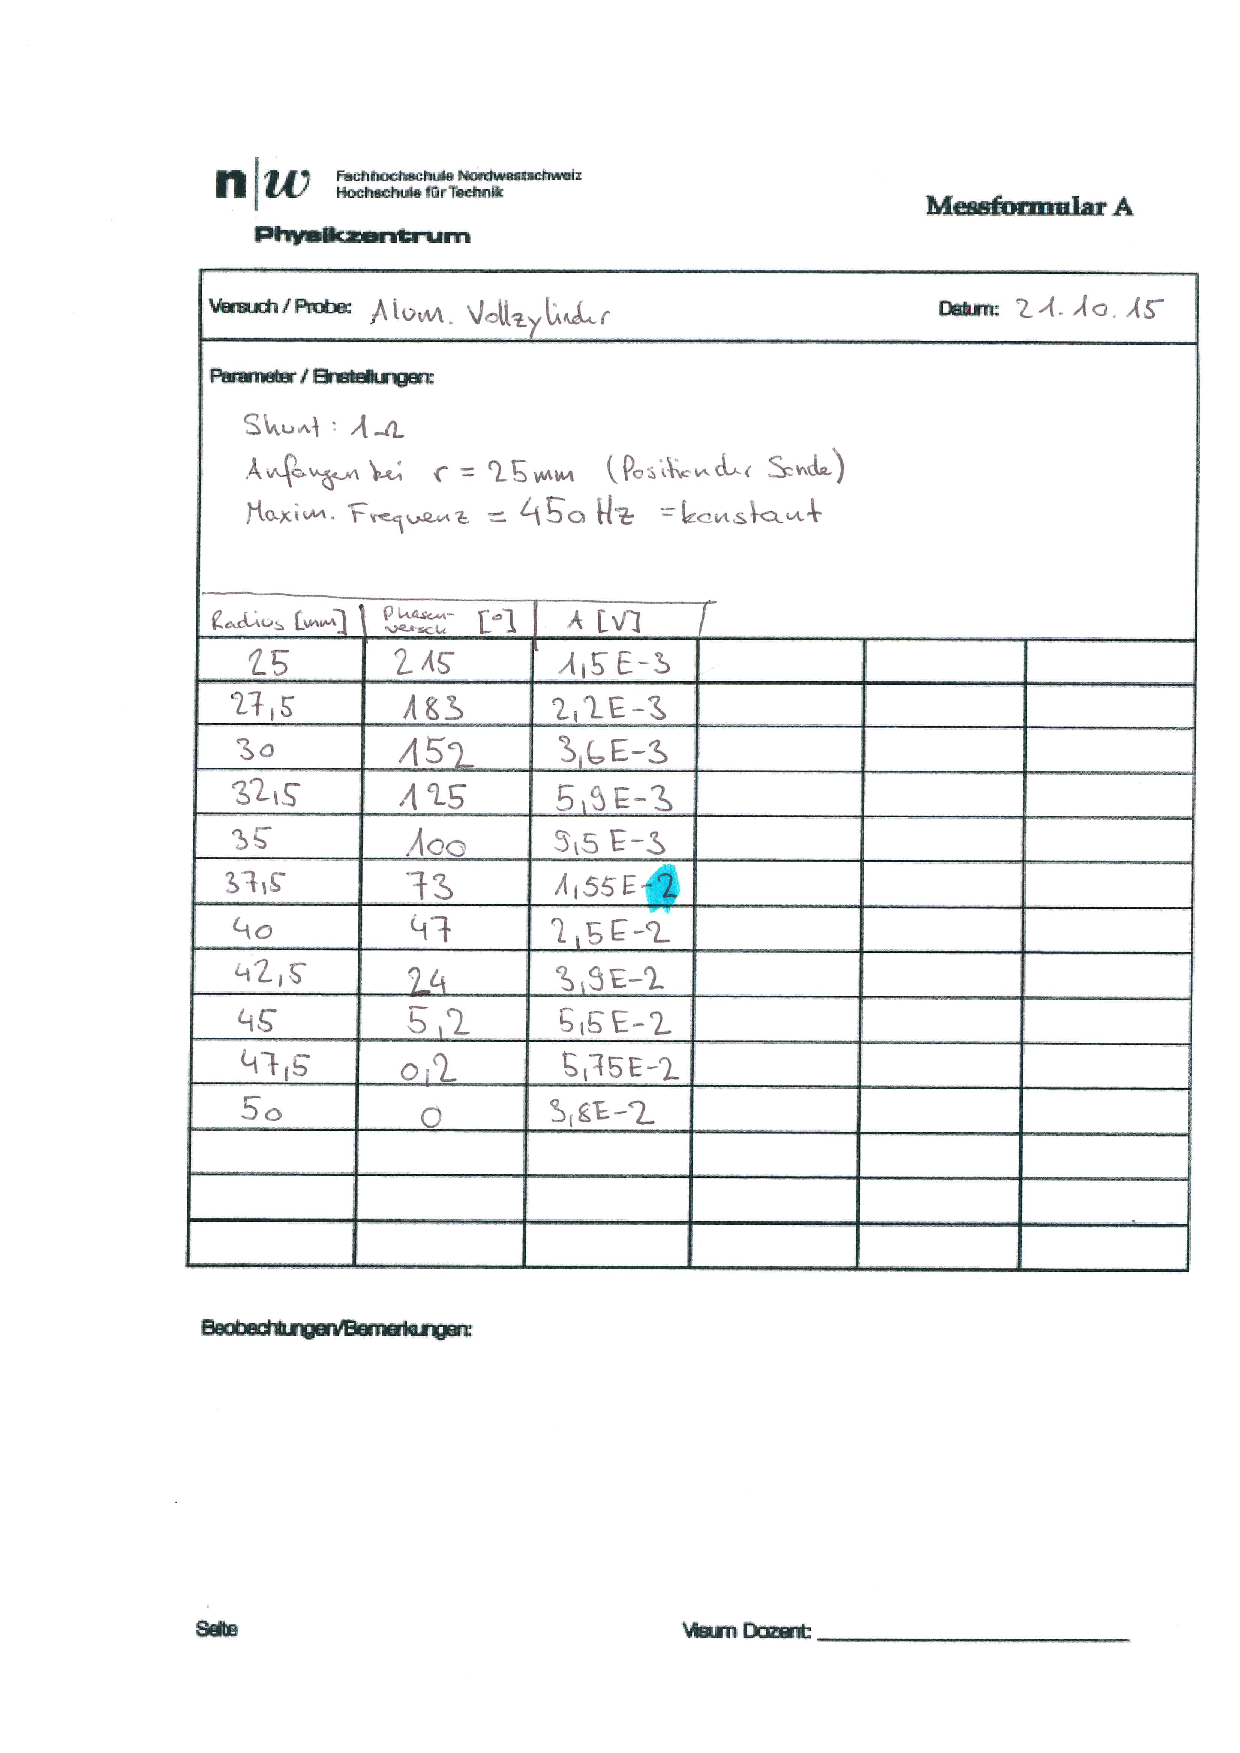
\includepdf[pages=-]{pdf/messprotokolle.pdf}
